% ProductieTechnologie-Samenvatting-RubenRyckaert.tex
% Simple layout template with helpers for chapters, a formularium, and an easy figure helper.

\documentclass[a4paper,11pt,twoside]{report}
\usepackage{../../school-macros}


% De faculteitsregel en de opmaak zitten in \maketitle (school-macros.sty);
% hier alleen nog de inhoud.
\title{Productietechnologie}
\subtitle{Samenvatting}
\author{Ruben Ryckaert}
\date{\today}

\begin{document}
\maketitle
\begin{abstract}
    Deze samenvattingen zijn beschikbaar op GitHub waar je kunt bijdragen aan verbeteringen: \url{https://github.com/KUL-Industriele-ingenieurs/Samenvattingen-Ku-leuven-Industriele-ingenieurs}

    Je bent helemaal vrij en ik raad je zelf aan om info toe te voegen aan de documenten als je de uitleg niet goed vindt.
    Je leert je vak en je raakt dan ook bekend met LaTeX wat handig is voor later.
\end{abstract}
\tableofcontents

\printformularium


\chapter{Inleiding}
\textbf{Wat is Productietechnologie?}

Productietechnologie gaat over het produceren van goederen. Hier komt veel bij te pas:
niet alleen verschillende technieken en machines, maar ook kosten,
snelheid en kwaliteit spelen een rol.

Deze samenvatting geeft een overzicht van de belangrijkste begrippen en technieken.

\textbf{Hieronder verschillende productietechnieken,}

\begin{itemize}
    \item Gieten
          \begin{itemize}
              \item Zandgieten
              \item Spuitgieten
          \end{itemize}
    \item Frezen
    \item Lassen
          \begin{itemize}
              \item CO2-lassen
              \item MIG/MAG, TIG, \ldots
          \end{itemize}
    \item Vonkerosie
    \item Waterstraalsnijden
    \item Chemisch bewerken
    \item 3D-printen
    \item Draaien
    \item Snijden
    \item Ponsen
    \item Stralen
          \begin{figure}[htbp]
              \centering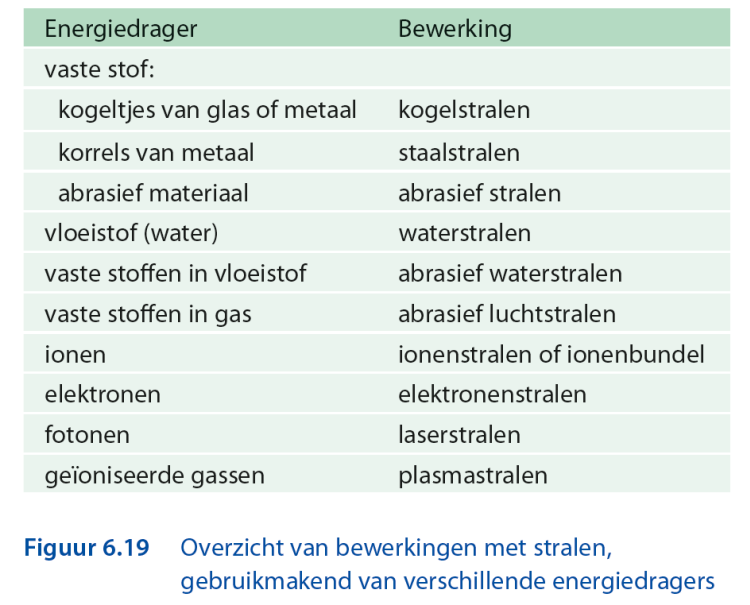
\includegraphics[width=0.5\textwidth]{assets/straalbewerkingen.png}
              \caption{Overzicht van bewerkingen met stralen, gebruikmakend van verschillende energiedragers}
              \label{fig:stralen_overzicht}
          \end{figure}
\end{itemize}

\section{Keuzes bij productie}

Bij produceren moet je uit al deze technieken kiezen welke het beste past.
Hoeveel producten moet ik maken en wat kost dat? Het hangt allemaal af
van de eisen die aan het product worden gesteld.

\begin{itemize}
    \item Kosten
    \item snelheid
    \item kwaliteit
    \item milieu
    \item veiligheid
    \item functionaliteit
    \item materiaal
    \item tolerantie
    \item oppervlaktekwaliteit
    \item aantal
    \item onderhoud
\end{itemize}

Al deze factoren zijn belangrijk bij het kiezen van een productietechniek.

\section{Passing}

\begin{conceptbox}[Passing]
    Passing is de maat voor de speling of de klemming tussen twee in elkaar passende onderdelen (zoals een as en een gat).
\end{conceptbox}

\begin{itemize}
    \item \textbf{Losse passing}: Er is altijd speling aanwezig tussen de onderdelen.
    \item \textbf{Nauwe passing (overgangspassing)}: De onderdelen sluiten zeer nauw aan, met een zeer kleine speling of een lichte klemming.
    \item \textbf{Perspassing}: Er is altijd overlapping (klemming); de onderdelen worden met kracht in elkaar geperst.
\end{itemize}

\section{Tolerantie}

\begin{conceptbox}[Tolerantie]
    Tolerantie is de toelaatbare afwijking op een nominale maat.
    Geen enkel onderdeel kan exact op de gewenste maat worden gemaakt; toleranties geven de grenzen aan waarbinnen het
    product functioneel blijft.
\end{conceptbox}

Afhankelijk van de toleranties heb je verschillende soorten passing:
\begin{itemize}
    \item \textbf{Losse passing}: Grote tolerantie, veel speling.
    \item \textbf{Perspassing}: Zeer kleine of negatieve tolerantie, klemming.
\end{itemize}

Je hebt hier \belangrijk{Maattoleranties} en \belangrijk{Vormtoleranties}.
\begin{itemize}
    \item \textbf{Maattoleranties}: Afwijkingen in afmetingen (lengte, diameter, \ldots).
    \item \textbf{Vormtoleranties}: Afwijkingen in geometrische vormen (rechtheid, vlakheid, rondheid, \ldots).
\end{itemize}

Algemeen bij nominale maten:
je definieert je nominale maat (de gewenste maat) en daarrond een boven- en een ondergrens.

De tolerantie is gewoon het verschil tussen die twee grensmaten:

\frm{Tolerantie}{T = D_{\max} - D_{\min}}{waarbij $T$ de tolerantie is [\si{mm}],
    $D_{\max}$ de bovenste grensmaat (maximummaat) [\si{mm}] en $D_{\min}$ de onderste grensmaat (minimummaat) [\si{mm}].}




\begin{figure}[htbp]
    \centering
    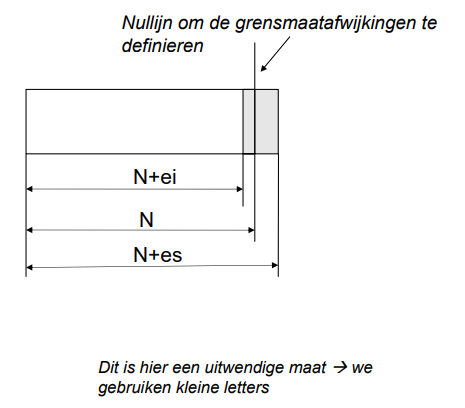
\includegraphics[width=0.4\textwidth]{assets/nominalematen.png}
    \caption{Nominale maten met boven- en ondergrens.}
    \label{fig:nominale_maten}
\end{figure}
\FloatBarrier


Afhankelijk van de tolerantie heb je tolerantieklassen (IT-klasse).

\begin{conceptbox}[IT-klasse]
    \textbf{De IT-klasse (International Tolerance grade)}
    geeft de nauwkeurigheid van een maat aan. Hoe lager het IT-nummer, hoe strakker de tolerantie.
    \newline
\end{conceptbox}

De plaats van de tolerantiezone t.o.v.\ de nominale maat hangt af van de letter.
Een hoofdletter geldt voor inwendige maten (gaten), een kleine letter voor uitwendige maten (assen).

\begin{voorbeeld}[H7]
    H7 zie je in de figuur hieronder. H is een hoofdletter, dus het gaat om een inwendige maat (een gat).
    Bij inwendige maten heet de onderste afwijking EI en de bovenste ES.
    Voor H geldt $EI = 0$: de tolerantiezone begint precies op de nominale maat en ligt er volledig \emph{boven}.
    De 7 is de IT-klasse en bepaalt hoe breed die zone is.
\end{voorbeeld}

\begin{voorbeeld}[h6 en js6]
    Bij uitwendige maten (assen) heten de afwijkingen $es$ (boven) en $ei$ (onder).
    \begin{itemize}
        \item \textbf{h}: $es = 0$, dus de tolerantiezone ligt volledig \emph{onder} de nominale maat.
              Samen met H7 geeft dit de klassieke spelingpassing H7/h6.
        \item \textbf{js}: symmetrisch verdeeld, $es = +IT/2$ en $ei = -IT/2$. De zone ligt dus half boven
              en half onder de nominale maat.
    \end{itemize}
\end{voorbeeld}

\begin{figure}[htbp]
    \centering
    
\includegraphics[width=0.45\textwidth]{assets/image1.png}\hfill
    
\includegraphics[width=0.45\textwidth]{assets/image2.png}\hfill
    \caption{Tolerantie diagrammen voor inwendige, uitwendige en passing.}
    \label{fig:tolerantie_diagrammen}
\end{figure}
\FloatBarrier

\begin{figure}
    \centering
    
\includegraphics[width=1\textwidth]{assets/image3.png}
    \caption{Tabel IT-klassen}
    \label{fig:itklassen_voorbeeld}
\end{figure}

De ligging van de twee tolerantiezones bepaalt wat voor soort passing je krijgt:
\begin{itemize}
    \item \belangrijk{Positieve speling}: er blijft altijd ruimte tussen de onderdelen (losse passing).
    \item \belangrijk{Negatieve speling}: er is altijd klemming (perspassing).
    \item \belangrijk{Positieve én negatieve speling}: de zones overlappen gedeeltelijk, dus afhankelijk van
          het exacte stuk krijg je speling of klemming (overgangspassing).
\end{itemize}

Verschillende productietechnieken hebben verschillende haalbare toleranties.
\begin{figure}[htbp]
    \centering
    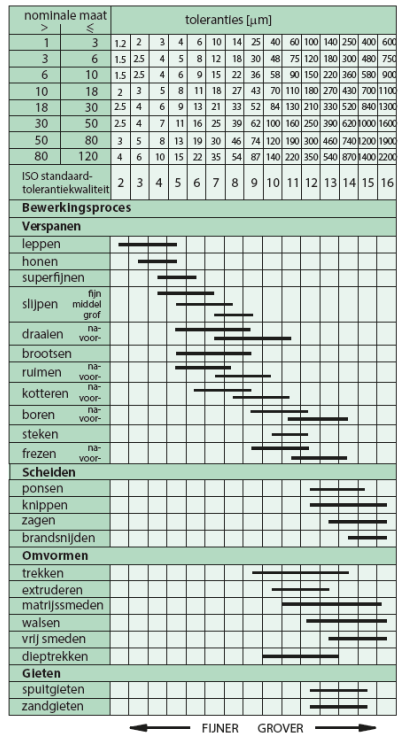
\includegraphics[width=0.8\textwidth]{assets/image86.png}
    \caption{Haalbare toleranties voor verschillende productietechnieken.}
    \label{fig:haalbaretoleranties.png}
\end{figure}
\FloatBarrier

\subsection{Kosten vs. Tolerantie}
Je moet kiezen welke tolerantie nodig is voor een product.
Precieze toleranties zijn duurder om te produceren.

\begin{figure}[htbp]
    \centering
    
\includegraphics[width=0.5\textwidth]{assets/image5.png}
    \caption{Kosten in functie van de tolerantiegraad.}
    \label{fig:kosten_vs_tolerantie}
\end{figure}


\section{Oppervlaktekwaliteit}

\begin{conceptbox}[Ruwheid]
    De oppervlaktekwaliteit wordt bepaald door de geometrische afwijkingen op microschaal (ruwheid).
    De belangrijkste parameters zijn $R_a$ (gemiddelde afwijking) en $R_z$ (gemiddelde top-dal hoogte).
\end{conceptbox}

\begin{itemize}
    \item Een ruw oppervlak is goedkoper om te produceren.
    \item Een glad oppervlak vereist nabewerkingen en is dus duurder.
    \item Textuur kan ook functioneel zijn (antislip, esthetisch, olie-retentie).
\end{itemize}

\begin{figure}[htbp]
    \centering
    
\includegraphics[width=0.45\textwidth]{assets/image6.png}
    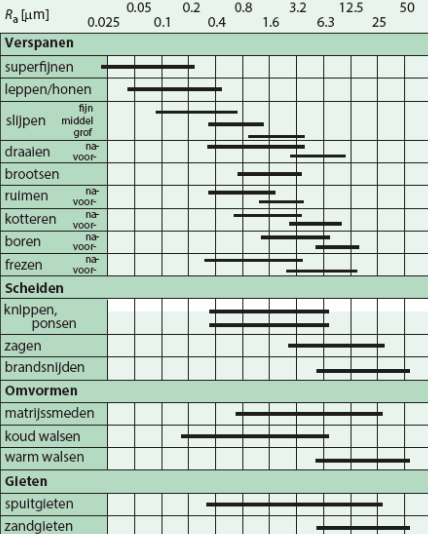
\includegraphics[width=0.45\textwidth]{assets/image7.png}
    \caption{Voorbeelden van verschillende oppervlaktekwaliteiten.}
    \label{fig:oppervlaktekwaliteiten}
\end{figure}
\FloatBarrier

\begin{theorieblok}[Oppervlakteparameters]
    \begin{itemize}
        \item \textbf{Gemiddelde ruwheid ($R_a$)}: De gemiddelde absolute afwijking van het oppervlak ten opzichte van de middellijn over een bepaalde lengte.
        \item \textbf{Gemiddelde top-dal hoogte ($R_z$)}: Het gemiddelde van de vijf grootste top-dal hoogten binnen een meetlengte.
        \item \textbf{Maximale ruwheid ($R_{max}$)($R_t$)}: De grootste top-dal hoogte binnen een meetlengte.
    \end{itemize}
\end{theorieblok}

Verschillende productietechnieken hebben verschillende haalbare oppervlaktekwaliteiten.

\begin{warningbox}[EXAMEN CHECKLIST: INLEIDING]
    \begin{itemize}
        \item \textbf{Passingen}: Ken het verschil tussen losse, nauwe en perspassingen en hun functie.
        \item \textbf{Toleranties}: Begrijp de diagrammen en de relatie tussen IT-klasse en nauwkeurigheid.
        \item \textbf{Kosten vs. Tolerantie}: Leg uit waarom de kosten exponentieel stijgen bij nauwere toleranties.
        \item \textbf{Oppervlaktekwaliteit}: Begrijp de parameters $R_a$ en $R_z$ en de economische impact van gladde oppervlakken.
        \item \textbf{Proceskeuze}: Ken de criteria (kosten, snelheid, kwaliteit, aantal) voor het kiezen van een techniek.
    \end{itemize}
\end{warningbox}

\chapter{Materialen}

Dit hoofdstuk gaat over de effecten van verschillende materialen op productietechnieken en het effect van de techniek op de materiaalstructuur.

\begin{figure}[htbp]
    \centering
    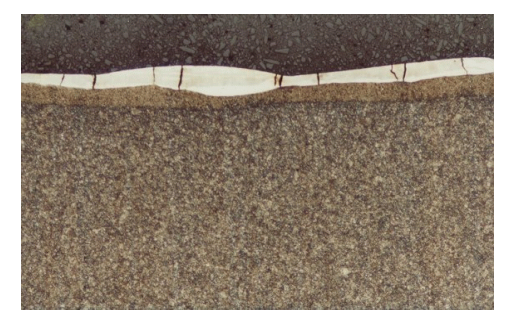
\includegraphics[width=0.5\textwidth]{assets/image9.png}
    \caption{Effect van thermische processen op de microstructuur van materialen.}
    \label{fig:image9}
\end{figure}

Er zijn verschillende materiaalgroepen:
\begin{itemize}
    \item \textbf{Metalen}: Goede geleiders, ductiel, vaak verspaanbaar of gietbaar.
    \item \textbf{Kunststoffen}: Lichtgewicht, lagere smelttemperaturen, ideaal voor spuitgieten.
    \item \textbf{Keramiek}: Extreem hard en hittebestendig, maar bros (moeilijk te verspanen).
    \item \textbf{Composieten}: Combinatie van eigenschappen, vaak lastig te bewerken door vezelstructuur.
\end{itemize}

\section{Vervorming}

\begin{conceptbox}[Vervormingsmodi]
    \begin{itemize}
        \item \textbf{Elastische vervorming}: Omkeerbare vervorming, het materiaal keert terug naar zijn originele vorm na ontlasting.
        \item \textbf{Plastische vervorming}: Blijvende vervorming, essentieel voor vormgevingsprocessen zoals buigen of ponsen.
    \end{itemize}
\end{conceptbox}

Elastische vervorming wordt beschreven door de wet van Hooke:
\frm{Hooke's law}
{\sigma = E \cdot \varepsilon}
{waarbij $\sigma$ de spanning is [\si{N/mm^2}], $E$ de elasticiteitsmodulus [\si{N/mm^2}] en $\varepsilon$ de rek [-].}

\begin{warningbox}[EXAMEN CHECKLIST: MATERIALEN]
    \begin{itemize}
        \item \textbf{Vervorming}: Leg het verschil uit tussen elastisch en plastisch en ken de overgang (vloeigrens).
        \item \textbf{Wet van Hooke}: Pas de formule toe en begrijp de betekenis van de E-modulus (stijfheid).
        \item \textbf{Materiaal vs. Proces}: Waarom is keramiek moeilijk te frezen maar goed te bewerken met EDM (indien geleidend)?
        \item \textbf{Thermische impact}: Begrijp dat warmte de materiaalstructuur permanent kan veranderen (harden, ontlaten).
    \end{itemize}
\end{warningbox}

\chapter{Verspanen: Algemeen}
\label{chap:Algemeen verspanen}
\textbf{Dit hoofdstuk is de basis van verspanen en is relevant voor alle verspaningstechnieken.}

Verspanen is het verwijderen van materiaal van een werkstuk. Dit kan door boren, frezen, draaien of slijpen,
\ldots Je begint met een ruw werkstuk en verwijdert materiaal totdat je de gewenste vorm en afmetingen hebt.

\textbf{Voordelen}
\begin{itemize}
    \item Hoge precisie
    \item Goede tolerantie
    \item Goede oppervlaktekwaliteit
    \item Flexibiliteit in ontwerp
\end{itemize}

\textbf{Nadelen}
\begin{itemize}
    \item Materiaalverlies
    \item Hogere kosten bij grote aantallen
    \item Langere productietijd
    \item Energie-intensief
    \item Vervuilend (spanen, koelvloeistof)
\end{itemize}

Bij verspanen kunnen verschillende tools gebruikt worden.
Deze tools hebben verschillende snijvlakken en geometrieën
die geschikt zijn voor verschillende materialen en bewerkingen.

\begin{itemize}
    \item beitel
    \item frees
    \item boor
    \item slijpschijf
\end{itemize}

\section{Beitelbewerkingen}
Bij beitelbewerkingen wordt materiaal verwijderd door een scherpe
beitel over het werkstuk te bewegen.
Je hebt daarbij deze parameters:
\begin{itemize}
    \item Spaanhoek $\gamma$
    \item Vrijloophoek $\alpha$
    \item Wighoek $\beta$
    \item Snedediepte $a$ (hoeveel mm er verwijderd wordt in de diepte)
    \item Voeding $f$
    \item Snijsnelheid $v_c$
    \item Snedebreedte $b$ (breedte van de beitel)
    \item Snededikte $h$ (hoeveel materiaal er per keer wordt verwijderd)
    \item wrijvingscoëfficiënt $\mu$
\end{itemize}

\begin{figure}[htbp]
    \centering
    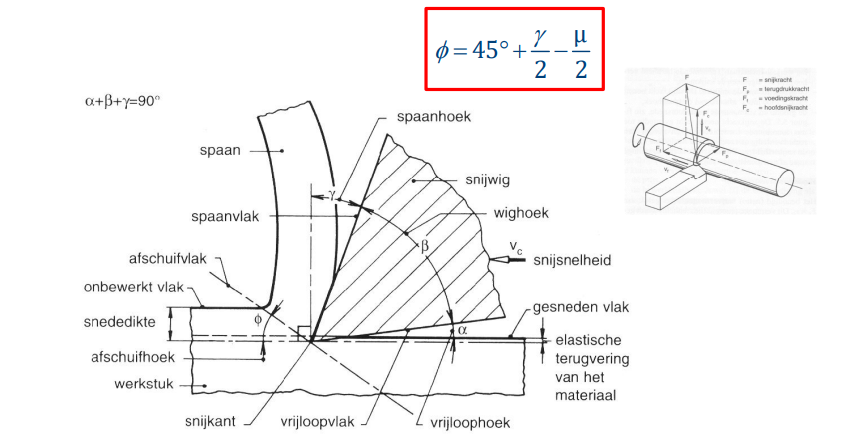
\includegraphics[width=0.7\textwidth]{assets/image10.png}
    \caption{Verwijdering van materiaal door een beitel $\to$ creëert spanen}
    \label{fig:image10}
\end{figure}


\begin{wrapfigure}[10]{r}{0.7\textwidth}
    \centering
    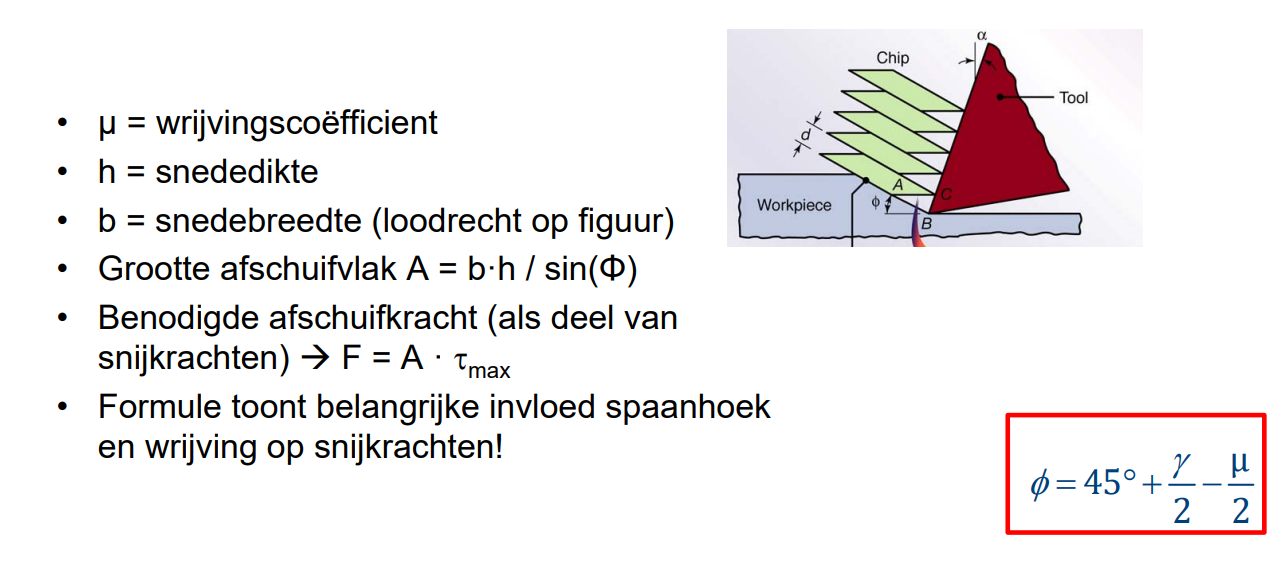
\includegraphics[width=\linewidth]{assets/image11.png}
    \caption{}
    \label{fig:image11}
\end{wrapfigure}


Bij het verspanen met een beitel ontstaan er \textbf{spanen}.
Spanen zijn kleine stukjes materiaal die worden verwijderd
van het werkstuk.
De grootte van de spanen wordt bepaald door de \textbf{snedediepte $a$}, de \textbf{voeding $f$},
de \textbf{spaanhoek $\gamma$} en de \textbf{wrijving} tussen spaan en beitel.
Zo meteen meer in detail hierover.


Het vormen van een spaan is een \textbf{plastische} vervorming van het weggenomen materiaal,
terwijl het achterblijvende oppervlak van het werkstuk ook nog \textbf{elastisch} terugveert.
Op de overgang tussen beide scheurt materiaal af, en dat geeft de fouten die je op het oppervlak ziet.

Je hebt verschillende soorten spanen:
\begin{itemize}
    \item \textbf{Continue:} Bij ductiele materialen en scherpe beitels. Goede oppervlaktekwaliteit.
    \item \textbf{Lamellen:} Bij hogere snededieptes of hardere materialen. Spaan breekt in dunne lagen.
    \item \textbf{Brokkelspanen:} Bij brosse materialen. De spaan breekt in kleine brokstukken.
\end{itemize}
\subsection{Primaire afschuifvlak (shear zone)}

\frm{Afschuifhoek}{\phi = 45^{\circ} + \dfrac{\gamma}{2} - \dfrac{\mu}{2}}
{waarbij $\phi$ de afschuifhoek is [$^\circ$], $\gamma$ de spaanhoek [$^\circ$] en $\mu$ de \emph{wrijvingshoek}
    [$^\circ$]. Let op: $\mu$ staat hier voor de hoek, niet voor de wrijvingscoëfficiënt; die twee hangen samen
    via $\tan\mu = $ wrijvingscoëfficiënt.}

De afschuifhoek bepaalt de richting waarin de spaan wordt afgeschoven.
Een grotere afschuifhoek geeft een kleiner afschuifvlak, dus een betere spaanvorming en minder kracht.

\frm{Afschuifvlak (shear zone) A}{A = \frac{b \cdot h}{\sin\phi}}
{waarbij $A$ het afschuifvlak is [\si{mm^2}], $b$ de snedebreedte [\si{mm}], $h$ de snededikte [\si{mm}] en $\phi$ de afschuifhoek
        [$^\circ$].}
\vspace{1cm}

\begin{figure}[htbp]
    \centering
    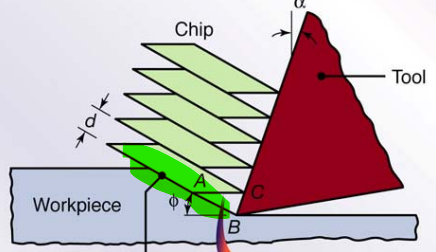
\includegraphics[width=0.4\textwidth]{assets/image20.png}
    \caption{}
    \label{fig:image20}
\end{figure}

\frm{Afschuifkracht}{F = A \cdot \tau}
{waarbij $F$ de afschuifkracht is [\si{N}], $A$ het afschuifvlak [\si{mm^2}] en $\tau$ de schuifspanning [\si{N/mm^2}].}

Grotere spaanhoek $\gamma$ $\to$ kleiner afschuifvlak $A$ $\to$ minder kracht $F$ nodig om spaan te vormen.


\subsection{Secundaire afschuifvlak (shear zone)}
Spanen gaan verwijderd worden en daarbij treedt wrijving op tussen spaan en beitel. Dit is het secundaire afschuifvlak
(vlak tussen spaan (groen) en beitel (rood)).
Als je met \textbf{negatieve spaanhoeken $\gamma$} werkt, dan is er veel meer wrijving tussen de spaan en de beitel (Je contact tussen spaan en beitel is groter).

De belangrijkste snijhoeken bij verspanen zijn \textbf{de spaanhoek $\gamma$, de wighoek $\beta$, en de vrijloophoek $\alpha$.}
Deze bepalen samen de benodigde kracht, de gereedschapsslijtage en de uiteindelijke oppervlaktekwaliteit.

\begin{itemize}
    \item \keyterm{Spaanhoek $\gamma$} $\to$ Een grotere hoek betekent dat er minder kracht nodig is voor de spaanvorming. Typische waarden liggen tussen -10° en 30°.
    \item \keyterm{Wighoek $\beta$} $\to$ Deze moet zo groot mogelijk zijn voor een goede sterkte en warmteafvoer. Grote wighoeken voeren de warmte sneller af, wat hogere voedingssnelheden toelaat.
          \begin{figure}[htbp]
              \centering
              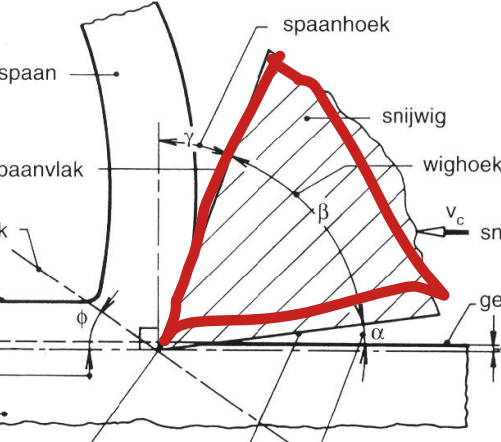
\includegraphics[width=0.4\textwidth]{assets/image12.png}
              \caption{Visualisatie van de wighoek $\beta$.}
              \label{fig:image12}
          \end{figure}
    \item \keyterm{Vrijloophoek $\alpha$} $\to$ Een grotere hoek zorgt voor minder wrijving tussen het werkstuk en de beitel. Typische waarden liggen tussen 6° en 10°. Zonder vrijloophoek (of bij hoeken rond de 0°) ontstaat er extreme wrijving en warmte.
          \begin{figure}[htbp]
              \centering
              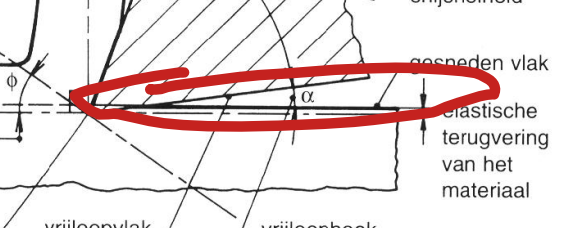
\includegraphics[width=0.4\textwidth]{assets/image14.png}
              \caption{Visualisatie van de vrijloophoek $\alpha$.}
              \label{fig:image14}
          \end{figure}
    \item \keyterm{Snedediepte $a$} $\to$ Hoe groter de diepte, hoe meer kracht er nodig is.
    \item \keyterm{Voeding $f$} $\to$ Hoe groter de voeding, hoe meer kracht er nodig is.
\end{itemize}

\begin{examenbox}
    Ken de drie belangrijkste hoeken ($\gamma, \beta, \alpha$) en hun effect op de snijkracht en warmteontwikkeling.
    Onthoud de typische bereiken: $\gamma \in [-10^\circ, 30^\circ]$ en $\alpha \in [6^\circ, 10^\circ]$.
\end{examenbox}

Deze verschillende hoeken hebben effect op elkaar. Dit is dus een optimalisatieprobleem.
Je moet afwegen wat de beste hoeken zijn voor jouw materiaal en bewerking.

\subsubsection{Extra info}

\begin{wrapfigure}{r}{0.45\textwidth}
    \centering
    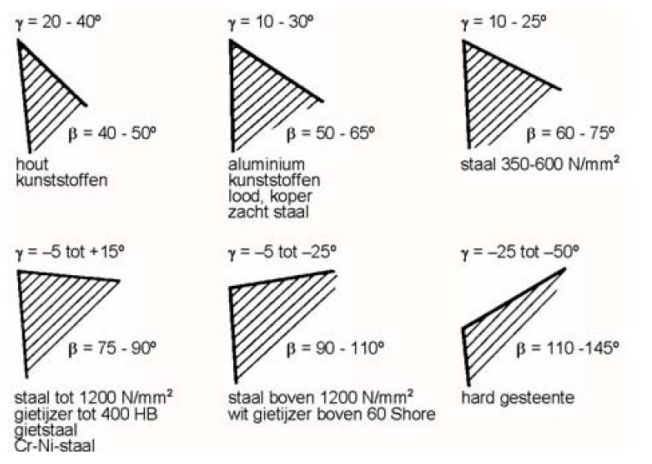
\includegraphics[width=\linewidth]{assets/image15.png}
    \caption{Verschillende spaanhoeken voor verschillende materialen}
    \label{fig:image15}
\end{wrapfigure}

De spaanhoek is enorm belangrijk. Een grote spaanhoek snijdt makkelijk
materialen zoals aluminium, koper, kunststof.
Voor hardere materialen zoals staal is een kleinere spaanhoek nodig
omdat het materiaal anders te hard is om te snijden en je moet veel te veel kracht zetten.
Negatieve spaanhoeken worden gebruikt voor zeer harde materialen.


Deze bewerkingen zijn allemaal met ductiele materialen.
Brosse materialen gaan snel afbrokkelen en hebben dus niet veel elastische vervorming.
Je moet dus druk uitoefenen op brosse materialen tijdens bewerking. Het materiaal gaat zich daardoor dan meer ductiel gedragen.
Hoe oefen je die druk uit? Door een kleine (of zelfs negatieve) spaanhoek te gebruiken,
maar die creëert dan weer veel wrijving en warmte.
Je moet dus een compromis zoeken tussen spaanhoek en wrijving.


\section{Beweging, snelheden en voedingen, temperaturen, slijtage}

Er zijn verschillende factoren die de kracht op je werkstuk bepalen:
\begin{itemize}
    \item Snijsnelheid (v)
    \item Voeding (f)
    \item Snedediepte (a)
    \item Snedebreedte (b)
    \item Snededikte (h)
\end{itemize}

\frm{Snijsnelheid}{v_c = \frac{\pi \cdot d \cdot n}{1000}}
{waarbij $v_c$ de snijsnelheid is [\si{m/min}], $d$ de diameter [\si{mm}] en $n$ het toerental [omw/min].
    De factor 1000 zet mm om naar m; werk je met $d$ in meter, dan valt die factor weg.}

\begin{figure}[htbp]
    \centering
    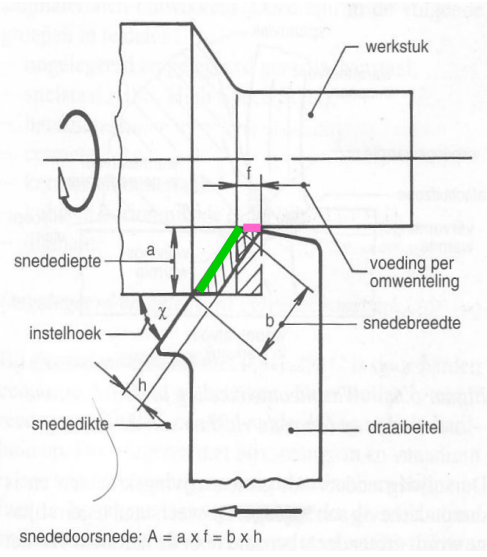
\includegraphics[width=0.3\textwidth]{assets/image16.png}
    \caption{Snededoorsnede bij beitelbewerking}
    \label{fig:image16}
\end{figure}

\frm{Snededoorsnede}{A_d = a \cdot b}{waarbij $A_d$ de snededoorsnede is [\si{mm^2}], $a$ de snedediepte [\si{mm}] en $b$ de snedebreedte [\si{mm}].}


\subsection{Krachten}
Tijdens het bewerken van materialen met een beitel komen er drie belangrijke krachten op het werkstuk en de beitel te staan:

\begin{itemize}
    \item \textbf{Hoofdsnijkracht ($F_c$)}: De kracht die nodig is om de spaan te vormen; dit is de grootste krachtcomponent.
    \item \textbf{Voedingskracht ($F_f$)}: De kracht die in de voedingsrichting werkt.
    \item \textbf{Terugdrukkracht ($F_p$)}: De kracht die nodig is om de beitel in het werkstuk te drukken.
          \begin{figure}[htbp]
              \centering
              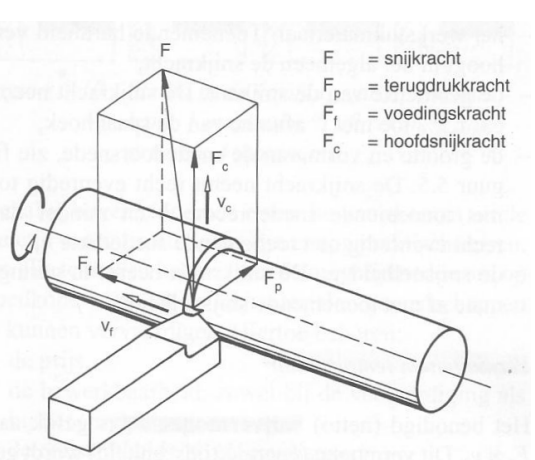
\includegraphics[width=0.4\textwidth]{assets/image17.png}
              \caption{Drie krachten bij verspanen: snijkracht $F_c$, voedingskracht $F_f$ en terugdrukkracht $F_p$.}
              \label{fig:krachten_verspanen}
          \end{figure}
\end{itemize}

\begin{examenbox}
    Onderscheid de drie krachten ($F_c, F_f, F_p$) en weet dat $F_c$ verantwoordelijk is voor het grootste deel van het verbruikte vermogen.
\end{examenbox}

\textbf{Waar gaat de toegevoerde energie naartoe?}
\begin{itemize}
    \item Spaanvorming (het plastisch vervormen zelf)
    \item Warmte in de spaan
    \item Warmte in het werkstuk
    \item Warmte in het gereedschap
\end{itemize}
Afhankelijk van de snijsnelheid $v_c$ en de voeding $f$ verschuift die verdeling.
\begin{figure}[htbp]
    \centering
    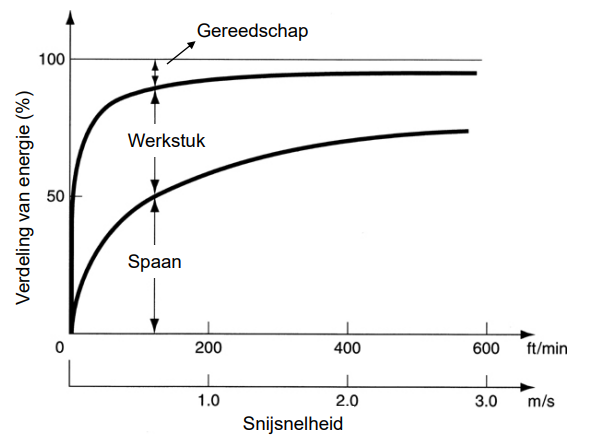
\includegraphics[width=0.5\textwidth]{assets/image21.png}
    \caption{Voeding of snijsnelheid in functie van de energieverdeling}
\end{figure}

\section{Factoren bij beitelbewerking}
De meeste dingen die we tot nu bekeken hebben, gelden bij ideale omstandigheden.
In werkelijkheid hebben beitelbewerkingen allemaal effecten op het materiaal. We bekijken er een paar.
\begin{examenbox}
    Hij gaat dit sowieso vragen. \textit{Wat zijn de effecten van beitelbewerkingen op het werkstuk en hoe kan je deze verbeteren of voorkomen?}
\end{examenbox}
\begin{enumerate}
    \item \textbf{Opbouwlaag (build-up edge/BUE)}:
          Een dunne, hard geworden laag metaal die zich bij lage snijsnelheden ($v_c < 20\,\si{m/min}$) aan de punt van de beitel opbouwt.
          Die opbouwlaag is scherper dan de beitel zelf en snijdt dus dieper, tot ze plotseling loslaat
          en stukken van het werkstukoppervlak meetrekt. Resultaat: een ruw, gerafeld oppervlak.

          \begin{examenbox}
              Onthoud de 3 belangrijkste manieren om BUE te voorkomen: verhoog de snijsnelheid ($v_c$),
              gebruik effectieve koeling/smering, en zorg voor een scherpe beitel met de juiste coating.
          \end{examenbox}

          \textbf{Verbeteren / Hoe voorkomen?:}
          \begin{itemize}
              \item Verhoog de snijsnelheid: bij hogere snelheden wordt het materiaal vloeibaarder en hecht het minder snel.
              \item Gebruik koeling of smering: vermindert adhesie tussen spaan en gereedschap.
              \item Kies geschikte gereedschapsmaterialen en coatings (bv. TiN/AlTiN).
              \item Controleer en vervang gereedschap regelmatig.
          \end{itemize}

    \item \textbf{Warmte}:
          Verspaningsprocessen genereren extreme hitte (tot wel 800-900°C).
          Zonder afvoer kan dit leiden tot thermische beschadiging zoals veranderingen in hardheid,
          ongewenste trekspanningen in het oppervlak en versnelde gereedschapsslijtage.

          Warmte wordt op drie locaties gecreëerd: het primaire afschuifvlak, het secundaire afschuifvlak (spaan-gereedschap contact) en
          het vrijloopvlak (gereedschap-werkstuk contact).

          Er zijn verschillende manieren om de warmte te beheersen:
          \begin{itemize}
              \item Koelen met koelvloeistof (emulsie) voor nauwkeurigheid.
              \item Smeren met olie voor hogere snelheden en minder wrijving.
              \item Spaanafvoer optimaliseren om te voorkomen dat de spaan de warmte teruggeeft aan het werkstuk.
          \end{itemize}

          \begin{figure}[htbp]
              \centering
              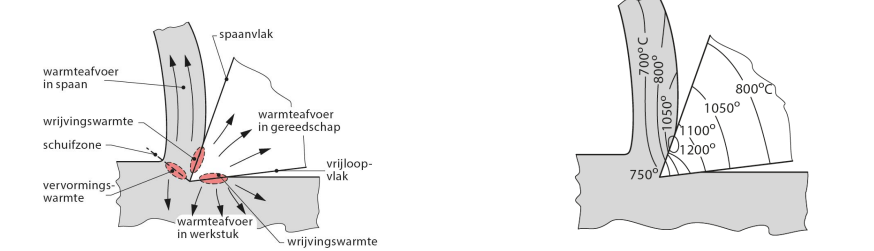
\includegraphics[width=1\textwidth]{assets/image18.png}
              \caption{Energieverdeling bij verspanen: de warmte wordt verdeeld over de spaan, de beitel en het werkstuk.}
          \end{figure}
          \FloatBarrier

    \item \textbf{Spaanvorming}

          Spanen kunnen het werkstuk beschadigen als ze niet goed worden afgevoerd.
          Dit kan leiden tot krassen en ruwheid.
          \begin{itemize}
              \item Continue spaan
              \item Lamelspaan
              \item Brokspaan
          \end{itemize}

    \item \textbf{Slijtage}

          Tijdens het bewerken van materialen slijt het gereedschap.
          Dit kan leiden tot een slechtere oppervlaktekwaliteit, hogere krachten,
          hogere temperaturen, enz.
          Slijtage kan veroorzaakt worden door:
          \begin{itemize}
              \item Vrijloopslijtage: door wrijving tussen gereedschap en werkstuk.
              \item Thermische slijtage: door hoge temperaturen die het gereedschap verzwakken
              \item Kerfslijtage: door herhaalde spanningsconcentraties aan de rand van het vrijloopvlak.
              \item Breuk: het afbreken van een stuk van de snijkant.
              \item Werkstukslijtage: de vrijloopvlakslijtage neemt toe naarmate de beitel verder verslijt.
              \item Neusslijtage: slijtage aan de punt van de beitel door hoge krachten en temperaturen.
          \end{itemize}

          \begin{figure}[htbp]
              \centering
              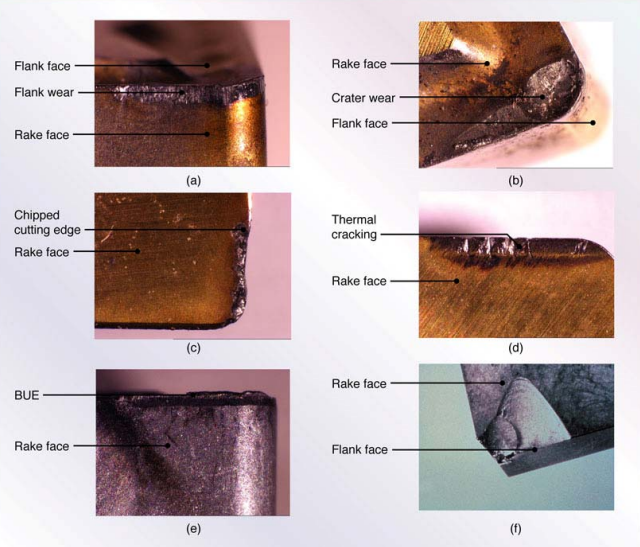
\includegraphics[width=0.40\textwidth]{assets/image23.png}
              \caption{Voorbeelden van slijtagevormen}
              \label{fig:slijtage_voorbeelden}
          \end{figure}
          \FloatBarrier

          \textbf{Je kunt slijtage verminderen door:}
          \begin{itemize}
              \item Gebruik van coatings op gereedschap (bv. TiN, AlTiN) om wrijving en hitte te verminderen.
              \item Optimaliseren van snijsnelheid, voeding en snedediepte om overmatige hitte en krachten te vermijden.
              \item Toepassen van koeling en smering om hitte af te voeren en wrijving te verminderen.
              \item Gereedschap met lood (Pb) gebruiken
                    \begin{figure}[htbp]
                        \centering
                        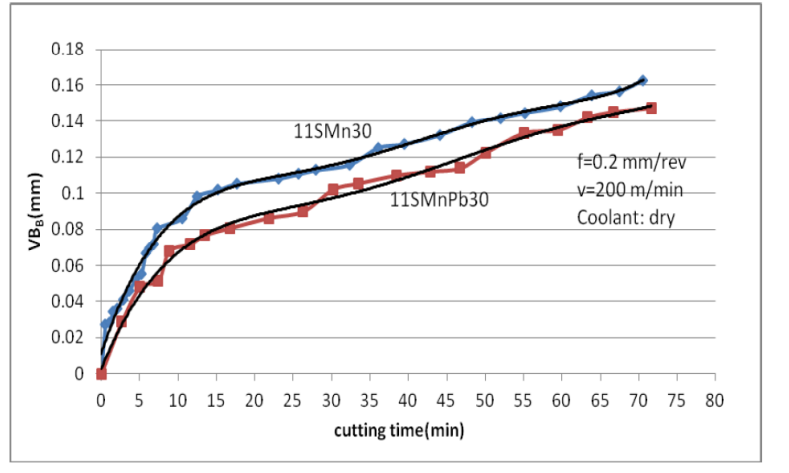
\includegraphics[width=0.7\textwidth]{assets/image22.png}
                        \caption{Minder slijtage met loodgecoat gereedschap}
                        \label{fig:image22}
                    \end{figure}
                    \FloatBarrier
                    Lood geeft minder slijtage omdat het smerende eigenschappen heeft $\to$ minder wrijving.
          \end{itemize}
\end{enumerate}


\section{Snijmaterialen}

\begin{wrapfigure}{r}{0.5\textwidth}
    \centering
    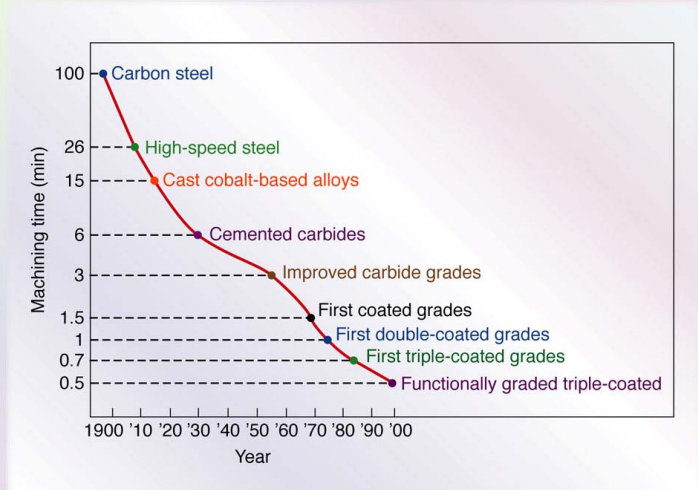
\includegraphics[width=\linewidth]{assets/image25.png}
    \caption{Ontwikkeling van snijmaterialen door de tijd heen.}
    \label{fig:snijmaterialen_ontwikkeling}
\end{wrapfigure}

Gereedschappen moeten een combinatie bieden van drie eigenschappen:
ze moeten \textbf{hard} zijn (ook bij hoge temperaturen), \textbf{ductiel/taai}
(om breuk bij stootbelasting te voorkomen) en \textbf{slijtvast}.

Dit is een ideaal materiaal maar eigenschappen zijn vaak tegenstrijdig.
Hardheid en taaiheid zijn vaak tegengesteld: hoe harder een materiaal, hoe brosser het is.
Je moet dus een compromis zoeken afhankelijk van de toepassing.

\begin{enumerate}
    \item \textbf{Snelstaal (HSS)} ($v_c \approx 10\text{--}30\,\si{m/min}$): Gehard staal met legeringselementen zoals wolfram of chroom. Goedkoop en taai, maar beperkt tot lage snelheden.
    \item \textbf{Hardmetaal (WC + Co)}: Bestaat uit wolframcarbide korrels in een kobaltmatrix. Behoudt zijn hardheid tot hogere temperaturen dan HSS.
    \item \textbf{Gecoat hardmetaal} ($v_c \approx 60\text{--}600\,\si{m/min}$): Dunne, gelaagde coatings (TiN, Al$_2$O$_3$) verbeteren de standtijd aanzienlijk.
    \item \textbf{Keramiek \& Diamant}: Extreem hard en hittebestendig, maar zeer bros. Diamant is ongeschikt voor staal: bij hoge temperatuur lost de koolstof van het diamant op in het ijzer, waardoor de snijkant wegvreet.
\end{enumerate}

\begin{examenbox}
    Ken de relatieve volgorde van snijmaterialen qua snijsnelheid en hardheid: HSS $\to$ hardmetaal $\to$ gecoat hardmetaal $\to$ keramiek $\to$ diamant.
\end{examenbox}


\begin{figure}[htbp]
    \centering
    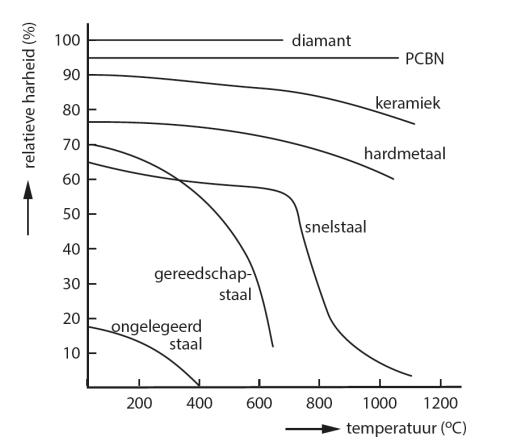
\includegraphics[width=0.5\textwidth]{assets/image24.png}
    \caption{Toepassingsgebieden van verschillende snijmaterialen in functie van snelheid en taaiheid.}
    \label{fig:snijmaterialen_overzicht}
\end{figure}
\FloatBarrier

Deze materialen zijn door de jaren heen ontworpen zoals in de figuur hieronder.

Je ziet dat machining time enorm daalt door de jaren
omdat je met \textbf{betere snijmaterialen} kan werken aan \textbf{hogere snelheden} $v_c$
en met \textbf{minder slijtage.}

\subsection{ISO-classificatie van snijmaterialen}
Snijmaterialen worden volgens ISO-normen in groepen ingedeeld op basis van het werkstukmateriaal:
\begin{itemize}
    \item \textbf{P} (Blauw): Voor staal.
    \item \textbf{M} (Geel): Voor roestvast staal.
    \item \textbf{K} (Rood): Voor gietijzer.
    \item \textbf{N} (Groen): Voor non-ferro metalen (aluminium, koper).
    \item \textbf{S} (Oranje): Voor superlegeringen (titanium).
    \item \textbf{H} (Grijs): Voor geharde materialen.
\end{itemize}

\begin{examenbox}
    Je moet op het examen de ISO-letters (P, M, K, N) kunnen koppelen aan het juiste werkstukmateriaal.
\end{examenbox}

\begin{figure}[htbp]
    \centering
    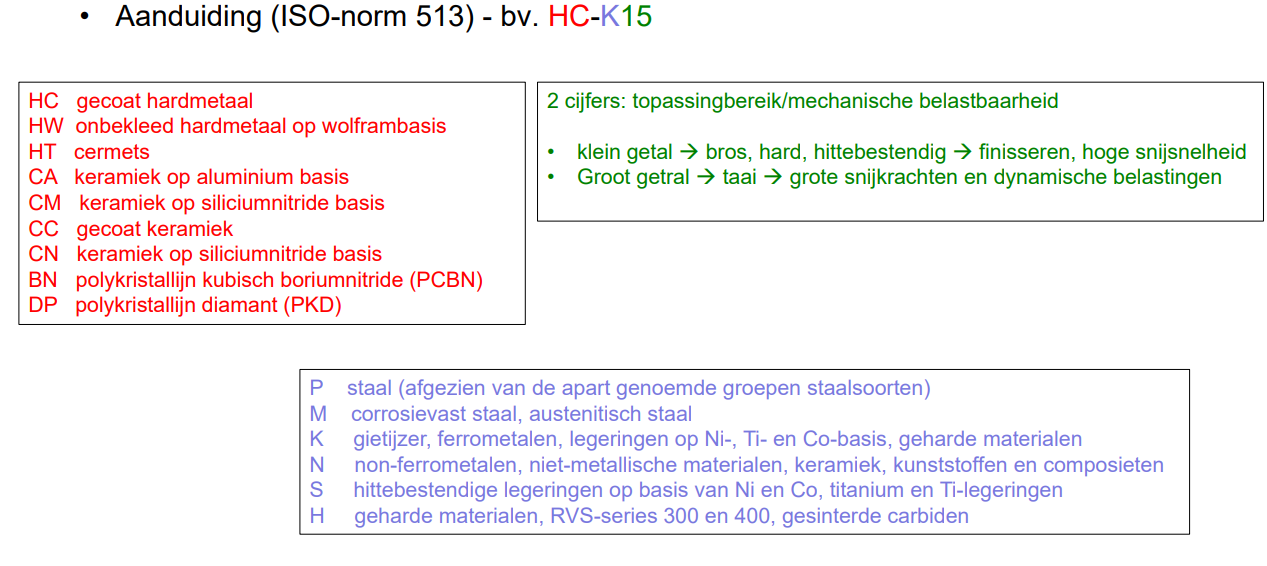
\includegraphics[width=0.8\textwidth]{assets/image26.png}
    \caption{Overzicht van de ISO-classificatie van snijmaterialen.}
\end{figure}

\begin{voorbeeld}
    In de figuur krijg je HC-K15. Snijmateriaal - materiaalgroep - grade
    \begin{itemize}
        \item H = Hardmetaal
        \item C = Coating
        \item K = Voor gietijzer
        \item 15 = Grade (hoger is harder)
    \end{itemize}
\end{voorbeeld}

\section{Optimale snijsnelheid}

Bij alle machines worden inserts gebruikt voor beitels.
Als beitels kapot gaan door slijtage, kan je die vervangen.
Je moet dus de optimale snijsnelheid kiezen
zodat je zo lang mogelijk met één insert kunt werken.

\begin{figure}[ht]
    \centering
    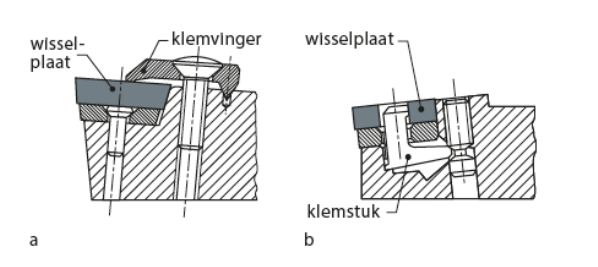
\includegraphics[width=0.5\textwidth]{assets/image27.png}
    \caption{Klemming van Inserts in een houder}
\end{figure}

Bij grotere snijsnelheden is er meer slijtage.

\textbf{Je kunt de levensduur van een gereedschap voorspellen met de formule van Taylor:}
\frm{formule van Taylor}{v_c\, T^n = C}{waarbij $C$ een materiaalconstante is [-], $n$ een materiaalconstante [-],
    $T$ de gereedschaplevensduur [\si{min}] en $v_c$ de snijsnelheid [\si{m/min}].}


Deze formule toont aan dat een kleine verhoging van de snijsnelheid $v_c$ leidt tot een zeer grote afname van de gereedschapslevensduur.

\begin{examenbox}
    Onthoud dat de exponent $n$ afhangt van het snijmateriaal: $n \approx 0{,}1\text{--}0{,}2$ voor HSS en $n \approx 0{,}2\text{--}0{,}4$ voor hardmetaal.
    Een kleinere waarde voor $n$ betekent dat de levensduur gevoeliger is voor veranderingen in snijsnelheid.
\end{examenbox}

\begin{voorbeeld}
    Je hebt deze waarden voor snijmateriaal staal Ck 45:
    \begin{itemize}
        \item $C = 300$
        \item $n = 0.22$
        \item Gewenste levensduur $T = 60\,\si{min}$
    \end{itemize}
    Bereken de optimale snijsnelheid $v_c$.
    \textbf{Oplossing:}
    \begin{align*}
        v_c & = \frac{C}{T^n}             \\
            & = \frac{300}{60^{0{,}22}}   \\
            & \approx \frac{300}{2{,}462} \\
            & \approx 121{,}9\,\si{m/min}
    \end{align*}
\end{voorbeeld}

\begin{voorbeeld}
    $n = 0{,}125$. Je verhoogt $v_c$ met 50\%. Hoeveel daalt $T$?
    \textbf{Oplossing:}
    \begin{align*}
        v_{c2}                         & = 1.5 \cdot v_{c1}                                                          \\
        v_{c1} T_1^n                   & = v_{c2} T_2^n                                                              \\
        v_{c1} T_1^n                   & = 1.5 \cdot v_{c1} T_2^n                                                    \\
        T_1^n                          & = 1.5 \cdot T_2^n                                                           \\
        \left(\frac{T_1}{T_2}\right)^n & = 1.5                                                                       \\
        \frac{T_1}{T_2}                & = 1{,}5^{\frac{1}{n}} = 1{,}5^{\frac{1}{0{,}125}} = 1{,}5^8 \approx 25{,}63 \\
        T_2                            & \approx \frac{T_1}{25{,}63}
    \end{align*}
    De levensduur daalt dus met een factor ${\sim}25{,}6$ bij een verhoging van de snijsnelheid met 50\%.
\end{voorbeeld}

\begin{figure}[htbp]
    \centering
    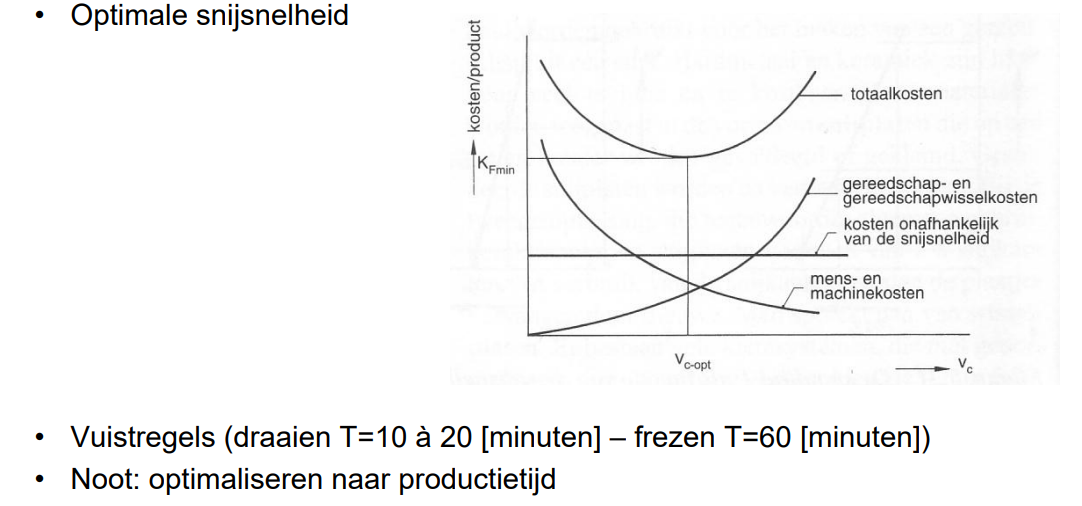
\includegraphics[width=0.8\textwidth]{assets/image28.png}
    \caption{Verband tussen snijsnelheid en levensduur volgens Taylor (log-log schaal).}
\end{figure}


\chapter{Verspanen: Draaien}
Draaien is een veelgebruikte verspaningstechniek waarbij een roterend werkstuk
wordt bewerkt met een beitel om materiaal te verwijderen en de gewenste vorm te creëren.

Je kunt hier verschillende bewerkingen mee uitvoeren:
\begin{enumerate}
    \item \textbf{Langsdraaien}: Het verwijderen van materiaal langs de lengteas van het werkstuk om de diameter te verkleinen.
    \item \textbf{Vlakdraaien}: Het creëren van een vlak oppervlak aan het uiteinde van het werkstuk.
    \item \textbf{Insteekdraaien}: Het snijden van een groef in het werkstuk (bv.\ voor een borgring).
    \item \textbf{Schroefdraadsnijden}: Het creëren van schroefdraad op het oppervlak van het werkstuk.
    \item \textbf{Afsteken:} De beitel gaat dwars (radiaal) naar binnen tot het afgewerkte stuk van de staaf loskomt.
    \item \textbf{Profieldraaien:} Met een vormbeitel wordt in één beweging een volledig profiel in het werkstuk gedraaid.
\end{enumerate}

\textbf{In de industrie:} Vandaag de dag wordt er veel gebruikgemaakt van computergestuurde machines.
CNC-draaien is een geautomatiseerd proces waarbij computergestuurde machines precies draaien volgens digitale ontwerpen. Veel conventionele machines en profieldraaien zijn vervangen door CNC-draaien.

\section{Het Draaiproces}

\begin{figure}[htbp]
    \centering
    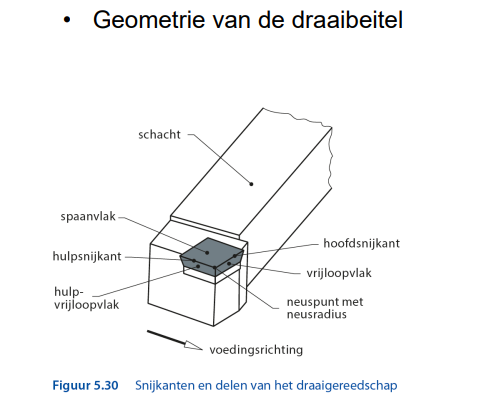
\includegraphics[width=0.45\textwidth]{assets/image29.png}
    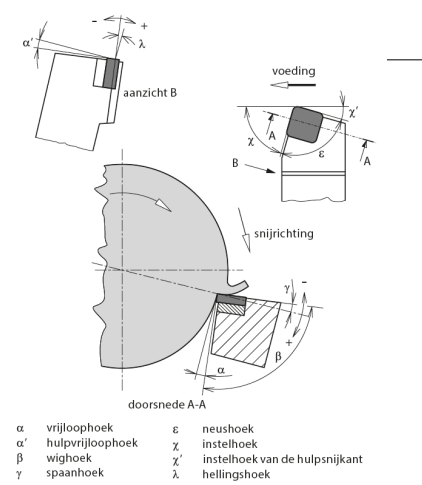
\includegraphics[width=0.45\textwidth]{assets/image30.png}
    \caption{Draaiproces}
\end{figure}
\FloatBarrier

\textbf{Hellingshoek}\
Omdat het werkstuk roteert terwijl de beitel axiaal doorschuift, beschrijft de snijkant geen vlakke cirkel
maar een schroeflijn. De helling van die schroeflijn is de \textbf{hellingshoek}.
Daardoor zit het bewerkte oppervlak onder een hoek t.o.v.\ de beitel en wordt je \emph{effectieve}
vrijloophoek $\alpha$ kleiner dan de geslepen vrijloophoek.

De hellingshoek volgt uit de voeding $f$ en de diameter $d$ ($\tan$(hellingshoek)$ = f/(\pi d)$).
Bij grotere voedingen wordt hij dus groter, en moet je een grotere vrijloophoek slijpen om te compenseren.

\begin{figure}[htbp]
    \centering
    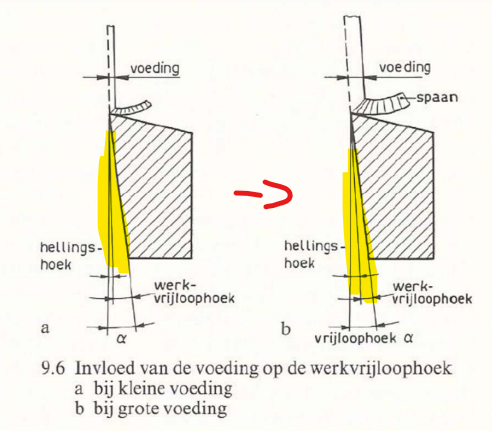
\includegraphics[width=0.4\textwidth]{assets/hellingshoek.png}
    \caption{Het effect van ronddraaien op de vrijloophoek}
    \label{fig:hellingshoek.png}
\end{figure}
\FloatBarrier

\section{Krachten bij Draaien}

\begin{conceptbox}[Kienzle-vergelijking]
    De Kienzle-vergelijking wordt gebruikt om de hoofdsnijkracht $F_c$ te berekenen.
    Het houdt rekening met de specifieke snijkracht van het materiaal en de spaanvorm (voeding en snedediepte).
\end{conceptbox}

\begin{wrapfigure}[16]{r}{0.4\textwidth}
    \centering
    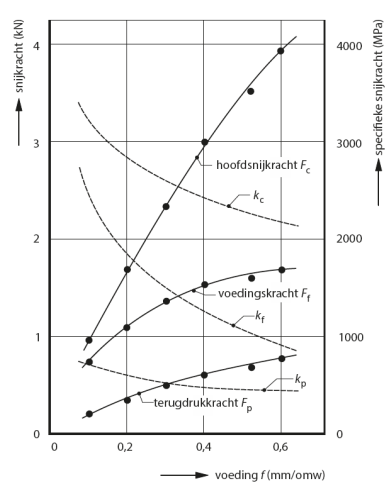
\includegraphics[width=0.4\textwidth]{assets/image31.png}
    \caption{Krachten bij draaien}
    \label{fig:image31}
\end{wrapfigure}
\FloatBarrier

Zoals vermeld in het hoofdstuk Verspanen: Algemeen (\ref{chap:Algemeen verspanen}) heb je drie krachten op je werkstuk:

\begin{enumerate}[leftmargin=*]
    \item De hoofdsnijkracht ($F_c$): kracht in de richting van de snijsnelheid.
    \item De voedingskracht ($F_f$): kracht tegengesteld aan de voedingsrichting.
    \item De terugdrukkracht ($F_p$): kracht die de beitel uit het werkstuk duwt.
\end{enumerate}

Afhankelijk van de voeding worden de krachten anders verdeeld:
bij grotere voeding neemt doorgaans $F_f$ sterker toe en verandert de verhouding $F_f/F_c$,
wat invloed heeft op opspanning, gereedschapbelasting en oppervlaktekwaliteit.
De figuur toont een steekproef van meetwaarden voor verschillende voedingen.

\begin{examenbox}
    Zorg dat je de volgende formules kunt uitleggen. De Kienzle-vergelijkingen komen overal
    bij verspanen terug.
\end{examenbox}

De hoofdsnijkracht wordt berekend met de formule van Kienzle:
\newline

\frm{Kienzle vergelijking Hoofdsnijkracht}{F_c = k_c \cdot a\cdot f^{(1-e)}}{waarbij $F_c$ de hoofdsnijkracht is [\si{N}], $k_c$ de snijkrachtcoëfficiënt [\si{N/mm^2}], $a$ de snedediepte [\si{mm}], $f$ de voeding [\si{mm/omw}] en $e$ de snijkrachtexponent [-].}

De snijkrachtcoëfficiënt $k_c$ is sterk afhankelijk van het materiaal van het werkstuk.
Typische waarden zijn $\sim 300\text{--}500\,\si{N/mm^2}$ voor aluminium
en $\sim 1500\text{--}2000\,\si{N/mm^2}$ voor staal.

\begin{examenbox}
    Je moet op het examen begrijpen hoe de snijkracht verandert bij een variërende voeding of snedediepte op
    basis van deze vergelijking.
    Begrijp ook de invloed van de exponent $e$ (die de kromming van de grafiek bepaalt).
\end{examenbox}

\frm{b: snedebreedte bij draaien}
{b = \frac{a}{\sin \kappa}}{met $b$ de snedebreedte [\si{mm}], $a$ de snedediepte [\si{mm}] en $\kappa$ de
    instelhoek [$^\circ$].}

\frm{h: snededikte bij draaien}
{h = f \cdot \sin \kappa}{met $h$ de snededikte [\si{mm}], $f$ de voeding [\si{mm/omw}] en $\kappa$ de
    instelhoek [$^\circ$].}

De optimale snijsnelheid bij draaien is afhankelijk van $k_c$

\frm{Optimale snijsnelheid bij draaien}{v_{c,\mathrm{opt}} = v_c(k_c)\cdot f^{-u}}
{waarbij $v_{c,\mathrm{opt}}$ de optimale snijsnelheid is [\si{m/min}], $f$ de voeding [\si{mm/omw}] en $u$ een exponent [-].}


\textbf{Aanvullende formules (zonder frm):}
\[
    \begin{aligned}
        P_c & = F_c\,v_c          \\
        P_m & = \dfrac{P_c}{\eta} \\
        v_c & = \pi\,d\,n         \\
        v_f & = f\,n              \\
        Q   & = a\,f\,v_c         \\
        M_c & = F_c\,\dfrac{d}{2}
    \end{aligned}
\]

Als $n$ in rev/min en $d$ in mm: $v_c\ ([\mathrm{m/min}]) = \pi\,\dfrac{d\,[\mathrm{mm}]}{1000}\;n\,[\mathrm{rev/min}]$.

\noindent
Korte uitleg en eenheden:
\begin{itemize}
    \item $P_c = F_c\,v_c$: vermogen is kracht maal snelheid (N·m/s = W). Als $v_c$ in m/min gegeven is, deel door 60 om naar m/s te gaan.
    \item $P_m = P_c/\eta$: rekening houden met mechanische/elektrische efficiëntie $\eta$ (dimensieloos); motorvermogen is altijd groter dan of gelijk aan het snijvermogen.
    \item $v_c = \pi d n$: op één omwenteling legt een punt op de omtrek een afstand $\pi d$ af; keer het aantal omwentelingen per tijd geeft lineaire snelheid. Let op eenheden (mm vs m, rev/min vs rev/s).
    \item $v_f = f n$: voedingssnelheid is voeding per omwenteling maal het aantal omwentelingen per tijd; gebruik mm/rev × rev/min = mm/min.
    \item $Q = a f v_c$: materiaalafname (volume per tijd) is snedediepte $\times$ voeding per omwenteling $\times$ \emph{snij}snelheid. Per omwenteling verwijder je immers een ring met doorsnede $a \times f$ over de hele omtrek. Reken $v_c$ om naar mm/min voor $\mathrm{mm}^3/\mathrm{min}$.
    \item $M_c = F_c (d/2)$: koppel is kracht maal arm (halve diameter als hefboom) → N·m.
\end{itemize}


Al deze formules zijn belangrijk om te begrijpen hoe de verschillende parameters bij draaien met elkaar in verband staan.
Een typische examenvraag is: ``met deze parameters en deze voeding, wat is de maximale snijsnelheid die ik kan gebruiken?''
Je kunt de verbanden logaritmisch plotten, zoals in de figuur hieronder, om die maximale snijsnelheid af te lezen.

\textbf{Zie dat alle formules in verband staan met de voeding.}

\begin{figure}[htbp]
    \centering
    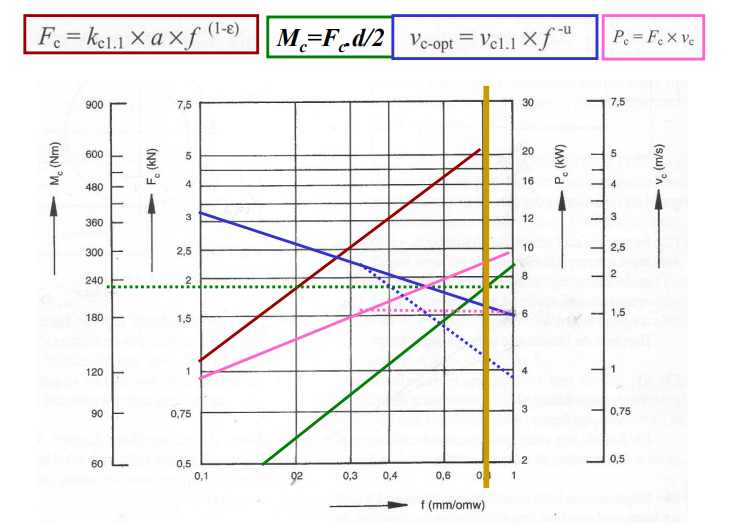
\includegraphics[width=0.8\textwidth]{assets/image32.png}
    \caption{Bepaling krachten, voeding of moment op werkstuk}
\end{figure}

Zo zie je hoe instelparameters zoals voeding, snijsnelheid en snedediepte in de industrie,
bepaald worden.

\section{Invloeden voeding \texorpdfstring{$f$}{f} en snedediepte \texorpdfstring{$a$}{a} op de kracht en snijsnelheid}



\begin{enumerate}
    \item \textbf{Softening effect (verzachting)}: Bij hogere voeding ontstaat meer warmte in het snijgebied.
          Die warmte maakt het oppervlak lokaal zachter, waardoor voor dezelfde snijsnelheid de snijkracht en voedingskracht doorgaans afnemen.
    \item \textbf{Build‑up edge (BUE)}: Bij lage snijsnelheden en bepaalde voedingen kan materiaal aan
          de snijkant aanhechten (BUE). Dit veroorzaakt tijdelijke pieken in de krachten en kan de oppervlaktekwaliteit verslechteren.
          Bij hogere voeding of snelheid neemt dit effect vaak af.
    \item \textbf{Snijkanthoek $\kappa$}: Het veranderen van de hoek van het snijvlak verschuift de richting en verdeling van de krachten.
          Sommige componenten (bijv. $F_c$) kunnen toenemen terwijl andere (bijv. $F_f$ of $F_p$) afnemen, waardoor
          de krachten anders verdeeld zijn.
    \item \textbf{Snedediepte $a_p$}: Een grotere snedediepte vergroot het verwijderde volume per
          omwenteling en verhoogt daardoor alle resulterende krachtcomponenten (snijkracht, voedingskracht, terugdrukkracht).
\end{enumerate}

\begin{figure}[htbp]
    \centering
    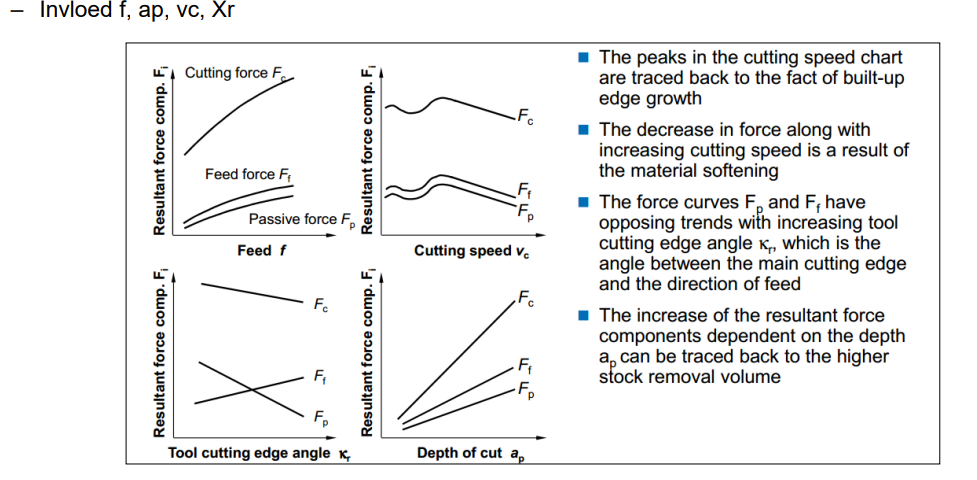
\includegraphics[width=1\textwidth]{assets/image33.png}
    \caption{Verschillende invloeden van voeding en snedediepte op de krachten bij draaien}
    \label{verschillende_invloeden_voeding_snedediepte}
\end{figure}

De krachten ($F_c$, $F_f$, $F_p$) volgen een machtsverband met de voeding, door de exponent $(1-e)$
in de Kienzle-vergelijking. Omdat $e > 0$ is die exponent kleiner dan 1: verdubbel je de voeding,
dan verdubbelt de kracht \emph{niet}, maar stijgt ze minder dan evenredig.
In een log-log-grafiek is dat een rechte met helling $(1-e)$.


\begin{examenbox}
    \textbf{Op het examen kan hij lege figuren geven en moet jij de effecten kunnen uitleggen.}
\end{examenbox}


\section{Spaanvorming bij Draaien}

Er zijn verschillende parameters die spaanvorming beïnvloeden
\begin{itemize}
    \item \textbf{Instelhoek $\kappa_r$}: De spaanslankheid $\dfrac{b}{h}$ hangt mede af van de instelhoek (met $b$ de snedebreedte en $h$ de snededikte).
    \item \textbf{Hellingshoek $\lambda$}: Een grotere hellingshoek kan de effectieve snedebreedte $b$ vergroten en daarmee de spaanslankheid beïnvloeden.
    \item \textbf{Snedediepte $a$}: Een grotere snedediepte vergroot doorgaans $b$ en verhoogt de spaanslankheid.
    \item \textbf{Voeding $f$}: Grotere voeding verhoogt de snededikte $h$, wat resulteert in dikkere spanen die moeilijker breken.
    \item \textbf{Materiaal}: Ductiele materialen veroorzaken vaak lange, samenhangende spanen; brosse materialen geven korte, brokkelige spanen.
    \item \textbf{Spaanhoek $\gamma$}: Een grotere spaanhoek geeft een grotere afschuifhoek en dus makkelijkere spaanvorming, maar ook langere, taaiere spanen die minder snel breken.
\end{itemize}

\frm{Spaanslankheid bij Draaien}{\dfrac{b}{h} = \dfrac{a}{f \cdot \sin \kappa_r}}{waarbij $b$ de snedebreedte [\si{mm}], $h$ de snededikte [\si{mm}], $a$ de snedediepte [\si{mm}], $f$ de voeding [\si{mm/omw}] en $\kappa_r$ de instelhoek [$^\circ$].}

\[h = f \cdot \sin\kappa_r\]

De snededikte $h$ bij draaien wordt bepaald door de voeding $f$ en de instelhoek $\kappa_r$. Een grotere voeding of een kleinere instelhoek resulteert
in een dikkere spaan, wat de spaanvorming beïnvloedt.

\[b = \dfrac{a}{\sin\kappa}\]

De snedebreedte $b$ bij draaien wordt bepaald door de snedediepte $a$
en de instelhoek $\kappa$. Een grotere snedediepte of een \emph{kleinere} instelhoek geeft
een bredere spaan (want $\sin\kappa$ staat in de noemer), wat de spaanvorming beïnvloedt.

\begin{figure}[ht]
    \centering
    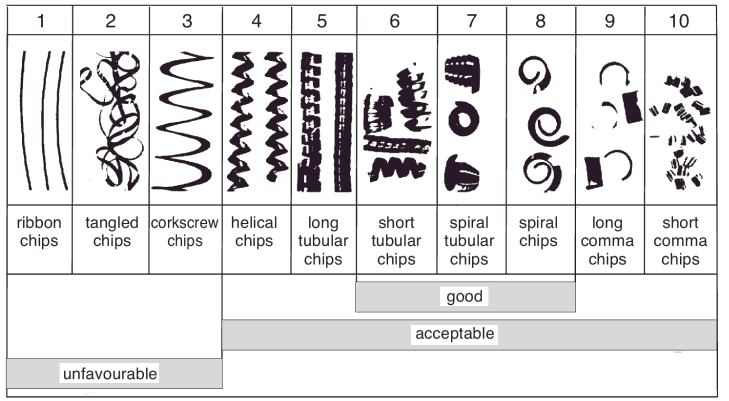
\includegraphics[width=0.45\textwidth]{assets/image34.png}
    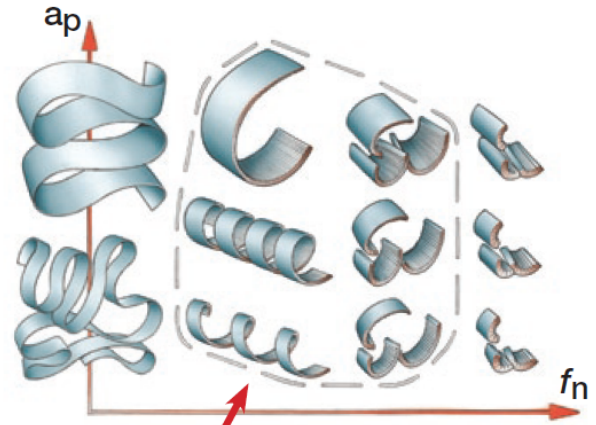
\includegraphics[width=0.45\textwidth]{assets/image35.png}
    \caption{Verschillende types spaanvorming bij draaien en welke goed zijn en welke parameters invloed hebben.}
\end{figure}



Om te lange spanen te vermijden worden spaanbrekers gebruikt:
inkepingen in het spaanvlak van de beitel die de spaan doen oprollen en breken in kleine stukken.

\begin{figure}[ht]
    \centering
    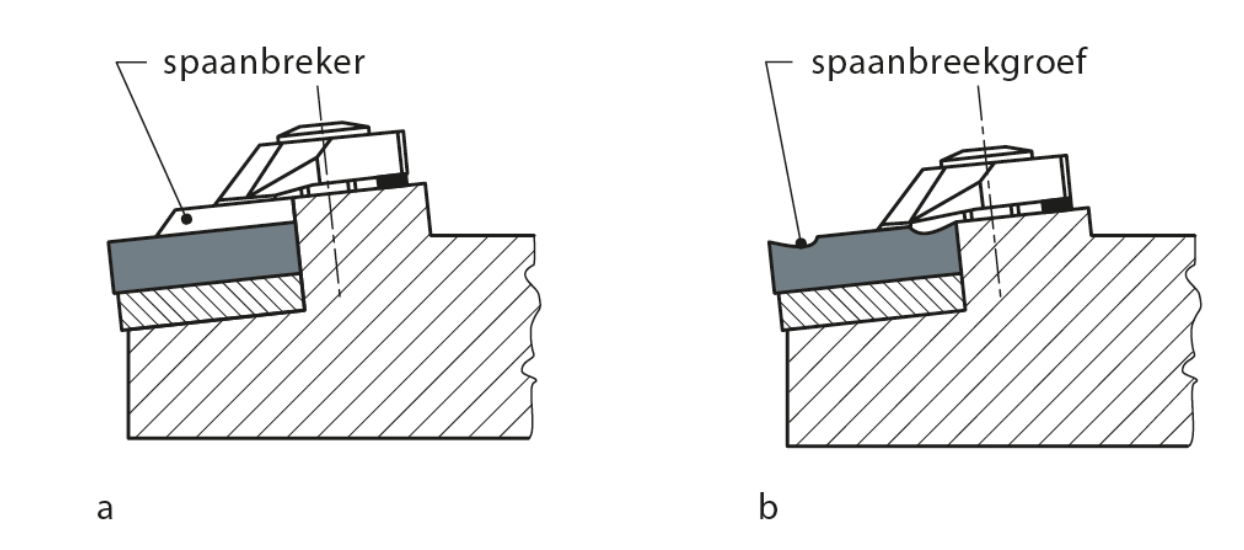
\includegraphics[width=0.5\textwidth]{assets/image36.png}
    \caption{Spaanbrekers in beitels}
\end{figure}

\section{Oppervlakteruwheid bij Draaien}

\begin{conceptbox}[Kinematische Ruwheid]
    Kinematische ruwheid is de theoretisch minimale ruwheid die ontstaat door de geometrie van de beitel (neusradius $r_\varepsilon$) en de verplaatsing per omwenteling (voeding $f$). In de praktijk is de werkelijke ruwheid hoger door trillingen en BUE.
\end{conceptbox}

De oppervlakteruwheid wordt gecreëerd door de beitel. De punt van de beitel is niet oneindig scherp maar
afgerond: dat is de neusradius $r_\varepsilon$.
Bij elke omwenteling schuift die afgeronde punt één voeding $f$ op en laat zo een rij kleine ribbels achter.
De ruwheid wordt dus bepaald door de neusradius $r_\varepsilon$ en de voeding $f$.

\begin{figure}[ht]
    \centering
    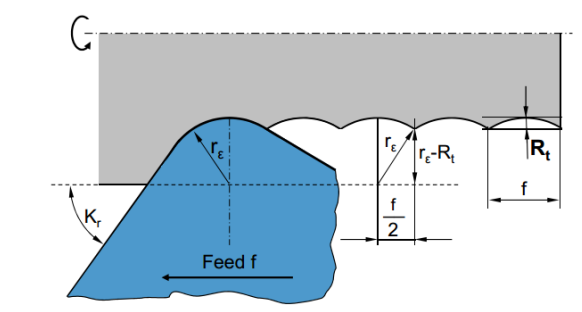
\includegraphics[width=0.45\textwidth]{assets/image37.png}
    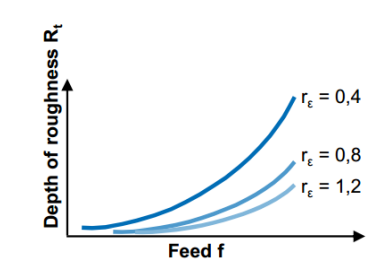
\includegraphics[width=0.45\textwidth]{assets/image38.png}
    \caption{}
\end{figure}
De oppervlakteruwheid wordt dus bepaald door de voeding en de neusradius.
\begin{itemize}
    \item $R_t$ is de \textbf{totale} hoogte van de ruwheid (piek tot dal).
    \item $R_a$ is de \textbf{gemiddelde} afwijking van de ruwheid.
\end{itemize}

\textbf{Kinematische ruwheid} volgt puur uit de geometrie en de kinematica van het systeem:
de neusradius en de voeding. Dit is de theoretische ondergrens.

\textbf{Procesruwheid} is de extra ruwheid door trillingen, gereedschapsslijtage en de
opbouwsnijkant (build-up edge, BUE).

\textbf{Totale ruwheid} is de som van beide: kinematische ruwheid $+$ procesruwheid.
De werkelijke ruwheid ligt dus altijd hoger dan wat de formules hieronder voorspellen.

\frm{Gemiddelde ruwheid bij draaien}{R_a = \dfrac{f^2}{32 \cdot r_\varepsilon}}{waarbij $R_a$ de gemiddelde ruwheid is [\si{mm}], $f$ de voeding [\si{mm/omw}] en $r_\varepsilon$ de neusradius van de beitel [\si{mm}].}
\frm{Totale ruwheid bij draaien}{R_t = \dfrac{f^2}{8 \cdot r_\varepsilon}}{waarbij $R_t$ de totale ruwheid is [\si{mm}], $f$ de voeding [\si{mm/omw}] en $r_\varepsilon$ de neusradius van de beitel [\si{mm}].}

\medskip
\noindent\textbf{Uitleg berekening neusradius.}
Denk aan de neusradius als een cirkelboog; de voeding per omwenteling \(f\) is de koorde van die boog.
De maximale hoogte van het profiel (piek tot dal) noemen we \(s\). Voor kleine voedingen geldt:
\begin{itemize}
    \item \textbf{Exact} (cirkelgeometrie): \(s = r_\varepsilon-\sqrt{r_\varepsilon^{2}-(f/2)^{2}}\).
    \item \textbf{Benadering} (veel gebruikt in de praktijk, eenvoudig te rekenen):
          \[
              R_t \approx s \approx \dfrac{f^{2}}{8\,r_\varepsilon},
              \qquad
              R_a \approx \dfrac{R_t}{4} \approx \dfrac{f^{2}}{32\,r_\varepsilon}.
          \]
\end{itemize}

Kort: ruwheid groeit met het kwadraat van de voeding en neemt af met de neusradius.

\smallskip
\noindent\textbf{Regel van duim \& voorbeeld.}
Geldigheid: de benadering klopt zolang \(f\) duidelijk kleiner is dan \(r_\varepsilon\) (praktisch: \(f \lesssim r_\varepsilon/2\)).
Voor \(f=0{,}2\ \si{mm}\) en \(r_\varepsilon=0{,}4\ \si{mm}\):
\[
    R_t\approx 12{,}5\ \si{\micro m},\qquad R_a\approx 3{,}1\ \si{\micro m}.
\]


\section{De Draaioperatie}

Draaien wordt met \textbf{verschillende beitels} gedaan die verschillende bewerkingen kunnen uitvoeren.
De punten van de beitels noemen we \textbf{inserts}.


\begin{figure}[htbp]
    \centering
    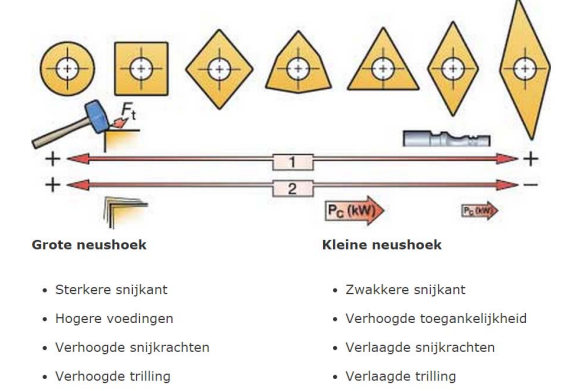
\includegraphics[width=0.8\textwidth]{assets/image39.png}
    \caption{Alle soorten Inserts voor verschillende draaioperaties}
\end{figure}
\FloatBarrier

De componenten worden in een draaimachine gestoken die deze beitels kan bewegen langs verschillende assen en het werkstuk
kan laten roteren.
Ze kunnen bewegen door AC (asynchrone) motoren of servomotoren die
de bewegingen zeer precies kunnen uitvoeren.
De snelheid van de motoren wordt getrapt door een tandwielkast.

\begin{figure}[htbp]
    \centering
    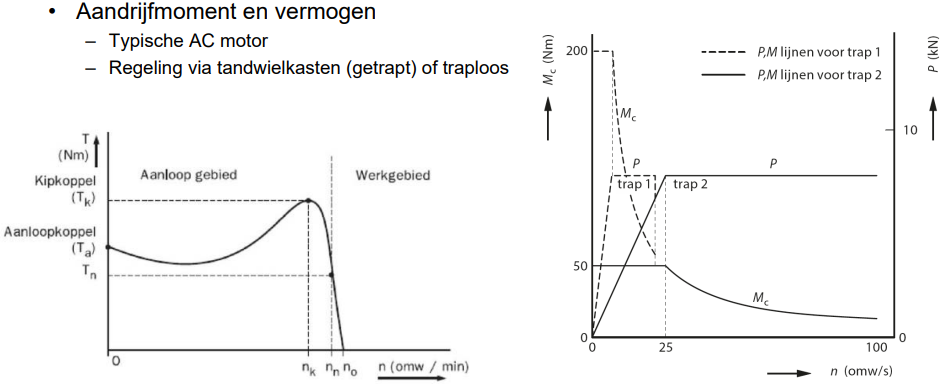
\includegraphics[width=1\textwidth]{assets/image40.png}
    \caption{Tandwielkast voor draaimachine}
\end{figure}
\FloatBarrier

Motoren werken vooral rond het steile deel van de koppel-toerentalcurve. Dat is interessant,
omdat je daar bij wisselende belasting toch ongeveer hetzelfde toerental behoudt.


\chapter{Verspanen: Boren, Fabricage en ronde gaten}
\section{Inleiding Boren}


Boren is een verspaningstechniek die wordt gebruikt om ronde gaten in materialen te maken.

\begin{conceptbox}[Volgorde voor precisiegaten]
    Boren (ruw gat) $\to$ Kotteren (centreren/vergroten) $\to$ Ruimen (finisseren op maat).
\end{conceptbox}

Belangrijke booroperaties zijn:

\begin{enumerate}
    \item \textbf{Boren}: Het primaire proces waarbij een boor wordt gebruikt om een rond gat te maken in het materiaal.
    \item \textbf{Kotteren}: Een nabewerkingsproces waarbij een kotter wordt gebruikt om de diameter van een bestaand
          gat te vergroten en de oppervlakteafwerking te verbeteren.
    \item \textbf{Ruimen}: Een proces waarbij een ruimer wordt gebruikt om de diameter van een bestaand gat te vergroten en de nauwkeurigheid en oppervlaktekwaliteit te verbeteren.
          Je kunt niet met normaal boren een accuraatheid van H7 bereiken. Hiervoor moet je ruimen gebruiken.
    \item \textbf{Tappen}: Het proces van het snijden van interne schroefdraad in een gat met behulp van een tap.
\end{enumerate}

\subsection{Boorgeometrie}

\begin{figure}[htbp]
    \centering
    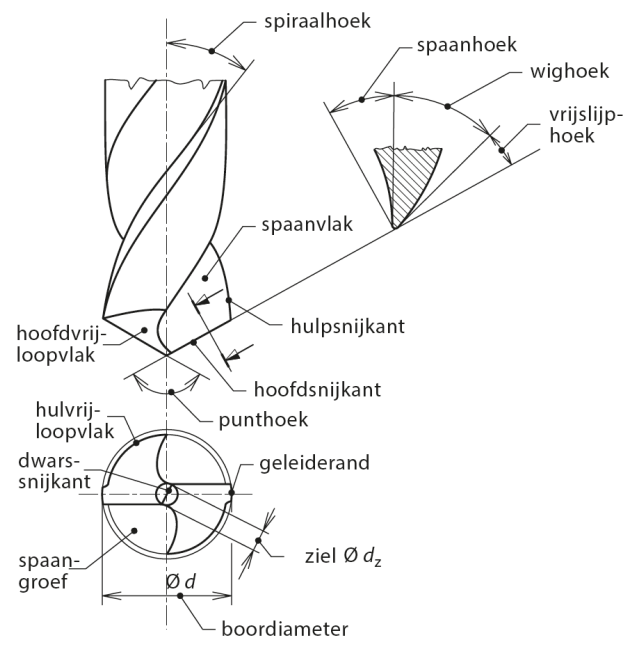
\includegraphics[width=0.45\textwidth]{assets/image41.png}
    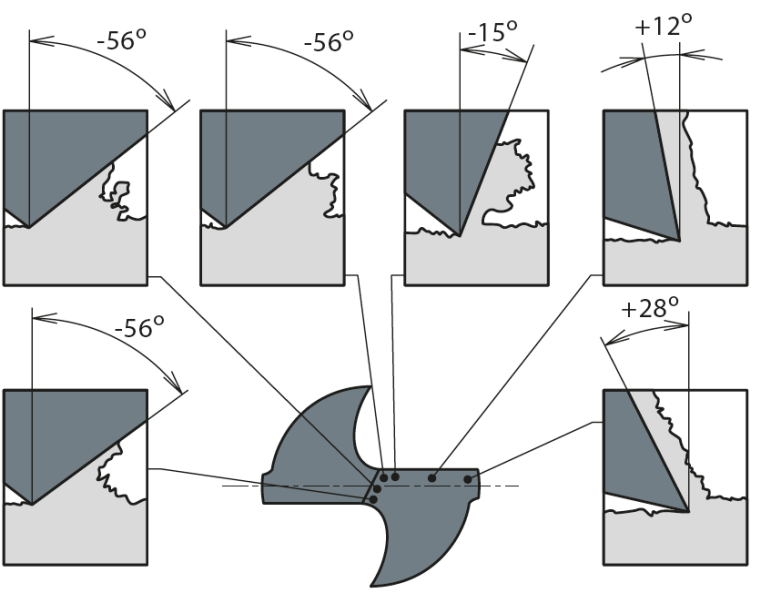
\includegraphics[width=0.45\textwidth]{assets/image42.png}
    \caption{Hoe de geometrie van een boor het werkstuk snijdt}
    \label{fig:boorgeometrie}
\end{figure}
\FloatBarrier

In de bovenste figuur zie je dat de spaanhoek $\gamma$ \emph{varieert} langs de snijkant van de boor.
Aan de buitenrand is hij positief, maar naar het centrum toe wordt hij steeds kleiner en uiteindelijk
sterk negatief (aan de dwarssnede). Hoe \emph{kleiner} de spaanhoek, hoe meer kracht je nodig hebt,
want de afschuifhoek $\phi$ wordt kleiner en het afschuifvlak $A$ wordt groter.
In het centrum van de boor wordt er dus nauwelijks gesneden en vooral geduwd.
\newline
\textit{Hou die twee uit elkaar: de afschuifhoek $\phi$ is de hoek tussen het werkstukoppervlak en het
    afschuifvlak; het afschuifvlak $A$ is het oppervlak waarover de plastische vervorming plaatsvindt.}

Negatieve spaanhoeken geven dus enorm veel kracht en maken het bewerken moeilijker, precies omdat de
afschuifhoek kleiner wordt.

Op een boor heb je belangrijke geometrie die andere functies hebben:
\begin{itemize}
    \item \textbf{Hoofdsnijvlak}: het primaire snijvlak dat het materiaal losmaakt.
          Draagt de meeste snijkracht en beïnvloedt oppervlaktekwaliteit en snijvermogen.
    \item \textbf{Hulpsnijvlak}: een secundair snijvlak nabij de punt dat afwerking en
          stabiliteit verbetert; draagt bij aan de lokale lastverdeling.
    \item \textbf{Spaanvlak}: het vlak waarlangs de spaan stroomt.
          Bepaalt spaanvorming, spaanafvoer en warmteontwikkeling (kolkslijtage kan optreden).
    \item \textbf{Vrijloopvlak}: het vlak dat niet in contact mag komen met het bewerkte oppervlak; met voldoende
          vrijloophoek voorkomt het wrijving en slijtage en behoudt maatnauwkeurigheid.
\end{itemize}

Doordat de boor tegelijk roteert én naar beneden gevoerd wordt, beschrijft elk punt van de snijkant
een schroeflijn in plaats van een vlakke cirkel. Hoe groter de voeding, hoe steiler die schroeflijn ligt.
De helling van die schroeflijn is de \textbf{spoedhoek} $\sigma$, met $\tan\sigma = f/(\pi d)$:
hij groeit dus met de voeding en is het grootst dicht bij het centrum (kleine $d$).
Die spoedhoek gaat af van de hoek die je geslepen hebt, waardoor de \emph{effectieve} vrijloophoek
kleiner is dan de \textbf{vrijslijphoek}.

\begin{figure}[htbp]
    \centering
    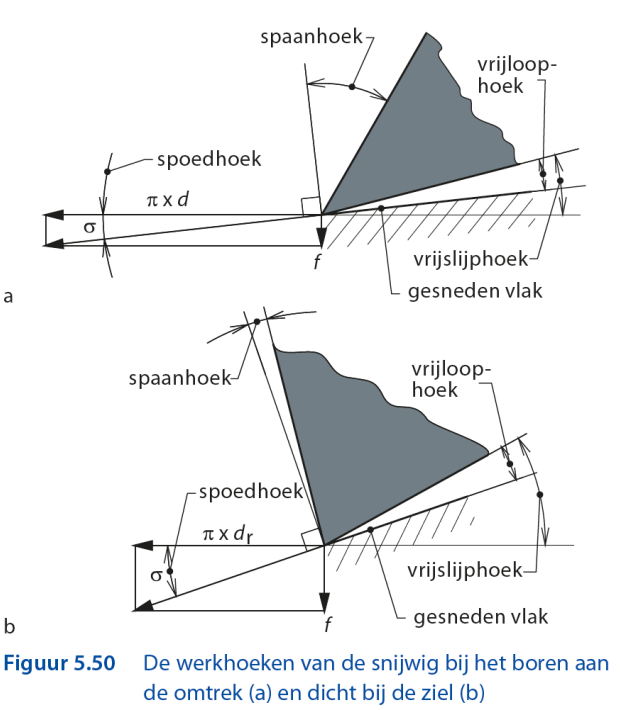
\includegraphics[width=0.4\textwidth]{assets/borenhoeken.png}
    \caption{Alle belangrijke hoeken bij boren}
    \label{fig:borenhoeken.png}
\end{figure}
\FloatBarrier

\textbf{De Vrijloophoek = vrijslijphoek - spoedhoek.}

Nog een keer alle belangrijke hoeken met hun functie en symbool:
\begin{itemize}
    \item \textbf{Spaanhoek} ($\gamma$): Bepaalt de snijweerstand en spaanvorming.
    \item \textbf{Afschuifhoek} ($\phi$): Beïnvloedt de kracht die nodig is om materiaal te verwijderen.
    \item \textbf{Vrijslijphoek} ($\alpha'$): De hoek tussen het horizontale vlak en de boor.
    \item \textbf{Vrijloophoek} ($\alpha$): De vrije hoek tussen boor en werkstuk.
    \item \textbf{Spoedhoek} ($\sigma$): De helling van de schroeflijn die de snijkant beschrijft, $\tan\sigma = f/(\pi d)$.
    \item \textbf{Wighoek} ($\beta$): De hoek tussen het hoofdsnijvlak en hulpsnijvlak.
\end{itemize}
\newpage

\section{Optredende krachten}

\begin{wrapfigure}[20]{r}{0.36\textwidth}
    \centering
    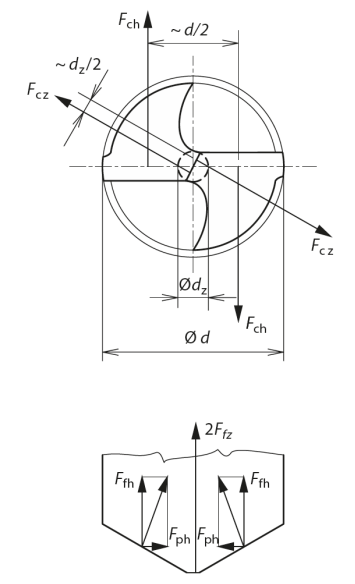
\includegraphics[width=0.36\textwidth]{assets/image43.png}
    \caption{Krachten op een boor}
    \label{fig:boren_krachten}
\end{wrapfigure}
\FloatBarrier

Net zoals bij draaien zijn er verschillende krachten die op het werkstuk
en de boor werken tijdens het boren. Deze worden met de vergelijking van Kienzle berekend.

Boren hebben een grote voedingskracht en een relatief klein snijmoment.
De axiale voeding is groot omdat de boor in het materiaal moet doordringen,
terwijl het snijmoment klein is door de geringe diameter.
Als de krachten niet in evenwicht zijn, ontstaat excentriciteit en scheef boren,
wat leidt tot slechte oppervlaktekwaliteit en onnauwkeurige gaten.

\begin{itemize}
    \item Grote axiale (voedings) kracht nodig om te penetreren.
    \item Klein snijmoment door kleine snijcirkel.
    \item Onevenwicht → scheef boren, variërende diameter en slechte afwerking.
\end{itemize}

\subsection{Gevolgen van onevenwichtige krachten}
Als de krachten niet in evenwicht zijn, wijkt je gatdiameter af.
Een gat van \SI{8,5}{mm} kan zo tot \SI{0,2}{mm} afwijken.


\section{Krachten bij Boren}
Net zoals bij draaien worden de krachten,
vermogens en momenten berekend met de vergelijking van Kienzle.

\textbf{Belangrijke krachten, vermogens en momenten bij boren:}
\frm{Voedingskracht}{F_f = k_f \cdot a \cdot f^{(1-e)}}{waarbij $F_f$ de voedingskracht is [\si{N}], $k_f$ de voedingskrachtcoëfficiënt [\si{N/mm^2}], $a$ de snedediepte [\si{mm}], $f$ de voeding [\si{mm/omw}] en $e$ de voedingskrachtsexponent [-].}
\frm{Verspaningsmoment}{M_c = C_m \cdot d^{x_M} \cdot f^{y_M}}{waarbij $M_c$ het verspaningsmoment is [\si{N.mm}], $C_m$ de momentcoëfficiënt [-], $d$ de diameter [\si{mm}], $f$ de voeding [\si{mm/omw}] en $x_M, y_M$ de momentexponenten [-].}
\frm{Vermogen bij boren}{P_c = M_c\,\omega = M_c \cdot 2\pi n}{waarbij $P_c$ het vermogen is [\si{W}], $M_c$ het verspaningsmoment [\si{N.m}] en $\omega$ de hoeksnelheid [\si{rad/s}].}

\section{Keuze van voeding}

Het belangrijkste bij de keuze van de voeding is de sterkte van de boor zelf.
Je berekent de torsie in de boor en leidt daaruit de maximaal toelaatbare voeding af.

\subsection{Torsie bij Boren}
\frm{Torsie bij Boren}{\tau = \dfrac{M_c\,\rho}{I_p}}{waarbij $\tau$ de schuifspanning is [\si{N/mm^2}], $M_c$ het verspaningsmoment [\si{N.mm}], $\rho$ de afstand van het centrum [\si{mm}] en $I_p$ het polair traagheidsmoment [\si{mm^4}].}

\begin{figure}[htbp]
    \centering
    \begin{tikzpicture}[
            scale=1.5,
            >=stealth,
            % Styles
            shaft/.style={line width=1.5pt, draw=black!80},
            stress/.style={->, red!80!black, thick},
            profileLine/.style={dashed, gray, thin},
            dim/.style={<->, gray, thin}
        ]

        % --- 1. DE AS (DOORSNEDE) ---
        \def\R{1.8}
        \draw[shaft, fill=gray!5] (0,0) circle (\R);
        \fill (0,0) circle (1.5pt) node[below left] {O};

        % --- 2. DE LINEAIRE SPANNINGSVERDELING (PROFIEL) ---
        % We tekenen de verdeling langs een horizontale as voor maximale duidelijkheid
        \draw[dashed, black!40] (0,0) -- (\R,0) node[midway, below] {$\rho$};

        % De "envelop" van de spanning (de schuine lijn die de lineaire groei toont)
        \draw[profileLine] (0,0) -- (\R, 1.0);

        % Reeks pijlen die de lineaire groei van tau tonen
        \foreach \x in {0.3, 0.6, 0.9, 1.2, 1.5, 1.8} {
                % Bereken de lengte van de pijl (lineair: lengte = constante * x)
                \pgfmathsetmacro{\len}{\x * (1.0 / \R)}
                \draw[stress] (\x, 0) -- (\x, \len);
            }

        % Label voor de maximale spanning aan de rand
        \node[anchor=south] at (\R, 1.0) {$\tau_{\text{max}}$};

        % --- 3. REPRESENTATIEVE PUNTEN (WILLEKEURIGE RADIUS) ---
        % Om aan te tonen dat het overal geldt, voegen we één willekeurige straal toe
        \def\ang{135}
        \def\rhoVal{1.3}
        \draw[gray, thin] (0,0) -- (\ang:\rhoVal) node[midway, below left, black] {$\rho$};
        \draw[stress, blue!70!black] (\ang:\rhoVal) -- ++(\ang+90:0.6) node[pos=1, left] {$\tau(\rho)$};

        % --- 4. FORMULES IN EEN NET KADER ---
        \node[draw=black!20, fill=white, rounded corners, anchor=west, align=left] at (2.2, 0.5) {
            $\tau(\rho) = \dfrac{M_c \cdot \rho}{I_p}$ \\[8pt]
            $\tau_{\text{max}} = \dfrac{M_c \cdot R}{I_p}$ \\[8pt]
            \small $I_p = \dfrac{\pi d^4}{32}$ \\[4pt]
            \small $d = 2R$
        };

        % --- 5. ONDERSCHRIFT ---
        \node[below=3cm, align=center, font=\itshape] at (1,0) {
            Spanningsverloop $\tau$ is lineair afhankelijk \\ van de afstand $\rho$ tot het centrum.
        };

    \end{tikzpicture}
    \caption{Torsiediagram: schuifspanning $\tau$ neemt lineair toe met de straal $\rho$; relevante formule staat buiten de doorsnede.}
    \label{fig:torsie_cirkel}
\end{figure}
Met het traagheidsmoment berekent als volgt (zie statica):
\newline
\textbf{Polair traagheidsmoment voor een cirkelvormige doorsnede:} $I_p = \frac{\pi d^4}{32}$

De combinatie van deze formules:

\frm{Maximaal toelaatbaar moment op de boor}{M_d = C_b \cdot d^{x_w}}{waarbij $M_d$ het maximaal toelaatbare
    moment is [\si{N.mm}] (volgt uit de torsiesterkte van de boor), $C_b$ een materiaal- en gereedschapsconstante,
    $d$ de diameter [\si{mm}] en $x_w$ de bijhorende exponent [-].}

\vspace{0.5cm}

\frm{Veiligheidsmarge op het moment}{M_c = a \cdot M_d}{waarbij $M_c$ het werkelijke verspaningsmoment is [\si{N.mm}],
    $M_d$ het maximaal toelaatbare moment [\si{N.mm}] en $a < 1$ de gekozen veiligheidsfactor [-].}


Samen met het verspaningsmoment:

\textbf{Afleiding van de maximale voeding $f_{\max}$ (twee methodes)}

\textbf{1) Via het schuifspanningscriterium:}
De maximale schuifspanning in de buitenvezel van een ronde doorsnede is
\[
    \tau_{\max}=\dfrac{16\,M_c}{\pi\,d^3}.
\]
Eis \(\tau_{\max}\le\tau_{\mathrm{allow}}\):
\[
    M_c \le \dfrac{\tau_{\mathrm{allow}}\,\pi\,d^3}{16}.
\]
Met \(M_c = C_m\,d^{x_M}\,f^{y_M}\) volgt
\[
    f_{\max} = \left(\dfrac{\tau_{\mathrm{allow}}\,\pi}{16\,C_m}\right)^{1/y_M} d^{(3-x_M)/y_M}.
\]

\textbf{2) Via het momentlimiet:}
Als \(M_c\le M_d=C_b\,d^{x_w}\) dan volgt
\[
    f_{\max} = \left(\dfrac{C_b}{C_m}\right)^{1/y_M} d^{(x_w-x_M)/y_M}.
\]

\textbf{Speciaal geval: lineair}
Wanneer \(y_M=1\) en \(x_w-x_M=1\) volgt
\[
    f_{\max} = \dfrac{C_b}{C_m}\; d,
\]
wat overeenkomt met de eenvoudige vorm \(f_{\max}=C\cdot d\).

\frm{Maximale voeding bij boren}{f_{max} = C \cdot d}{waarbij $C$ een constante is [-], $d$ de diameter [\si{mm}] en $f_{max}$ de maximale voeding [\si{mm/omw}].}



\frm{Kracht $F_f$ is de kracht recht naar boven bij een boormachine}
{F_f = C_f \cdot d^{X_f} \cdot f^{y_f}}{waarbij $F_f$ de voedingskracht is [\si{N}], $C_f$ de voedingskrachtcoëfficiënt [\si{N/mm^2}],
$d$ de diameter [\si{mm}], $f$ de voeding [\si{mm/omw}] en $X_f, y_f$ de voedingskrachtsexponenten [-].}

Deze kracht creëert een moment op de machine, dat het frame kan doen doorbuigen.
Dat speelt vooral bij C-vormige structuren.

\begin{figure}[htbp]
    \centering
    \begin{tikzpicture}[
            scale=1.3,
            >=stealth,
            every node/.style={font=\small},
            % Stijlen
            machine/.style={fill=gray!20, draw=black!80, line width=1.5pt, rounded corners=3mm},
            phantom/.style={draw=gray!40, line width=1.5pt, dashed, rounded corners=3mm},
            force/.style={->, ultra thick, red},
            dim/.style={<->, thin, gray!80, >=latex},
            ground/.style={fill, pattern=north east lines, draw=none}
        ]

        % --- Parameters ---
        \def\bedL{2.0}      % Lengte onderbed
        \def\colW{0.8}      % Breedte kolom
        \def\colH{4.0}      % Hoogte kolom
        \def\armL{2.5}      % Lengte bovenarm (incl kolombreedte)
        \def\armThick{0.8}  % Dikte arm/bed
        \def\rotAngle{4}    % Rotatiehoek voor deformatie

        % --- Coördinaten ---
        \coordinate (BaseBL) at (0,0); % Linksonder

        % --- 1. GHOST (Oorspronkelijke staat) ---
        % We tekenen de outline van de C-vorm in dashed grijs
        % Vorm: L-shape onder + kolom + arm boven
        \draw[phantom]
        (0,0) -- (\bedL, 0) -- (\bedL, \armThick) -- (\colW, \armThick)
        -- (\colW, \colH-\armThick) -- (\armL, \colH-\armThick)
        -- (\armL, \colH) -- (0, \colH) -- cycle;

        % Spindel ghost
        \coordinate (SpindleTopGhost) at (\armL - 0.4, \colH-\armThick);
        \draw[phantom, fill=none] (SpindleTopGhost) rectangle ++(0.3, -0.8);

        % --- 2. DEFORMATIE (Vervormde staat) ---
        % Rotatiepunt: ergens in de "oksel" van de C
        \coordinate (Pivot) at (\colW/2, \colH/2);

        \begin{scope}[rotate around={\rotAngle:(Pivot)}]
            % De "open gebogen" machine
            % We simuleren de buiging door het hele bovenstuk iets te kantelen t.o.v. onderstuk? 
            % Nee, bij C-frame buigt de 'rug' (kolom) naar achteren en de bek gaat open.
            % Eenvoudige benadering: roteer de hele C-vorm om een punt laag in de rug.

            \draw[machine]
            (0,0) -- (\bedL, 0) -- (\bedL, \armThick) -- (\colW, \armThick)
            -- (\colW, \colH-\armThick) -- (\armL, \colH-\armThick)
            -- (\armL, \colH) -- (0, \colH) -- cycle;

            % Spindel (Vast aan arm)
            \coordinate (SpindleTop) at (\armL - 0.4, \colH-\armThick);
            \draw[fill=white, draw=black, line width=1pt] (SpindleTop) rectangle ++(0.3, -0.8) coordinate (SpindleTip);
            \node[below, xshift=2mm] at (SpindleTip) {}; % dummy

            % Annotatie op frame
            \node at (\colW/2, \colH/2) [rotate=\rotAngle, text=gray] {\textbf{C-Frame}};
        \end{scope}

        % --- 3. FUNDERING ---
        \draw[ground] (-0.5,-0.3) rectangle (\bedL+0.5, 0);
        \draw[thick] (-0.5,0) -- (\bedL+0.5, 0);
        \node[below, text=gray] at (\bedL/2, -0.3) {Fundering};

        % --- 4. KRACHTEN & MOMENT ---
        % F_f duwt de arm en bed uit elkaar. Hier tekenen we F_f op de spindel (werkstuk duwt terug)
        % De positie is nu geroteerd.
        % We nemen het midden van de onderkant van de spindel rect.
        \coordinate (ForcePos) at ($ (SpindleTop) + (0.15, -0.8) $);
        \draw[force] ($(ForcePos) + (0, -0.8)$) -- (ForcePos) node[midway, right] {$F_f$};

        % Moment M: Buigend moment in de rug
        % Pijl die "open buigen" aangeeft
        \draw[->, ultra thick, orange!90!black] (-0.5, \colH/2 - 1) to[bend left=45] node[left] {$M$} (-0.5, \colH/2 + 1);

        % --- 5. AFMETINGEN & LABELS ---
        % Hoek theta (overdreven weergegeven)
        % Vergelijking verticale lijn
        \draw[dashed, gray] (0, \colH) -- (0, \colH + 1.0);
        \draw[->, thick] (0, \colH + 0.8) arc (90:{90+\rotAngle}:0.8) node[midway, above] {$\theta$};

        % Arm lengte l (keel diepte)
        % Vanaf binnenkant kolom tot spindel as
        \draw[dim] (\colW, \colH + 0.3) -- (\armL - 0.25, \colH + 0.3) node[midway, fill=white] {$l$};
        \draw[gray, thin] (\colW, \colH) -- (\colW, \colH + 0.5);
        \draw[gray, thin] (\armL - 0.25, \colH) -- (\armL - 0.25, \colH + 0.5);

        % --- 6. TEKSTVAK ---
        \node[align=left, anchor=north west, fill=white, inner sep=5pt, rounded corners] at (3.0, 3.5) {
            \textbf{C-Frame Buiging}\\
            Door $F_f$ buigt de kolom.\\
            De bek "opent" zich.\\
            \small $M = F_f \cdot l$
        };

    \end{tikzpicture}
    \caption{C\nobreak\-vormig frame: axiale voedingskracht $F_f$ op het werkstuk (pivot) veroorzaakt een lichte kanteling (\(\theta\)) rond het werkstuk; de gestippelde lijn toont de gedraaide positie van het frame.}
    \label{fig:Cframe_moment}
\end{figure}


\FloatBarrier


\section{Boormachines en booroperaties in de industrie}
\subsection{NC-gestuurde boormachines}
NC-gestuurde boormachines (Numerical Control) zijn computergestuurde machines die worden gebruikt voor het boren van gaten in materialen met
hoge precisie en herhaalbaarheid.
Deze machines maken gebruik van vooraf geprogrammeerde instructies
om de bewegingen van de boor en het werkstuk te regelen.
\newline

\subsection{Boren}
Hier zijn nog relevante boortypes en hun toepassingen:
\begin{itemize}
    \item \textbf{Toepassingen:} verspanen van gaten voor bevestigingsmiddelen, passingen en nabewerkingen (ruimen, kotteren); wordt ook gebruikt als pilot voor grotere bewerkingen.
    \item \textbf{Belangrijke parameters:} snijsnelheid $v_c$, voeding $f$, snedediepte $a$, koelmiddel en spaanvorm.
    \item \textbf{Veelvoorkomende boortypes:}
          \begin{itemize}
              \item \textbf{Centerboor / positioneerboor:} korte, stijve boor om een startpunt te maken (voorkomt uitlopen van de boor).
              \item \textbf{Steekboor (jobber / stub):} standaardboor voor algemene gaten; lengte en spiraaltype kies je afhankelijk van de diepte en de spaanafvoer.
              \item \textbf{Verzinkingsboor (countersink):} maakt een conische uitsparing voor schroefkoppen of voor ontbraamwerk.
              \item \textbf{Split-point / conische punt:} verbetert de centrering en vermindert het uitlopen van de boor bij het aanzetten.
          \end{itemize}
\end{itemize}

\begin{figure}[htbp]
    \centering
    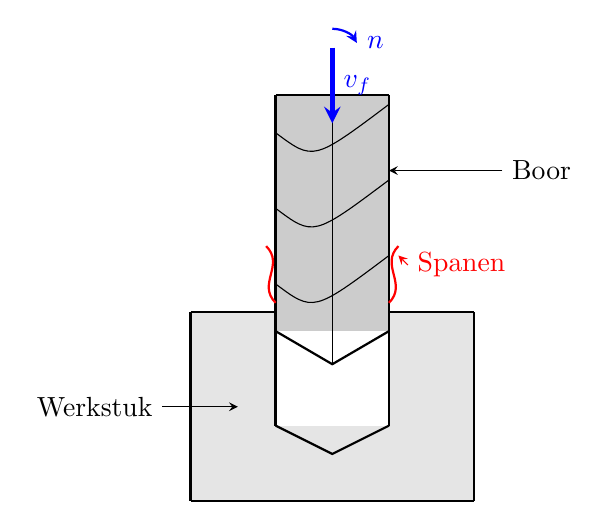
\begin{tikzpicture}[scale=1.2, >=stealth]
        % Werkstuk (doorsnede)
        \fill[gray!20] (-1.5, 0) rectangle (1.5, -2);
        \draw[thick] (-1.5, 0) -- (-0.6, 0);
        \draw[thick] (0.6, 0) -- (1.5, 0);
        \draw[thick] (-1.5, -2) -- (1.5, -2);
        \draw[thick] (-1.5, 0) -- (-1.5, -2);
        \draw[thick] (1.5, 0) -- (1.5, -2);

        % Gat
        \fill[white] (-0.6, 0) rectangle (0.6, -1.2);
        \draw[thick] (-0.6, 0) -- (-0.6, -1.2);
        \draw[thick] (0.6, 0) -- (0.6, -1.2);
        % Conische bodem van het gat
        \draw[thick] (-0.6, -1.2) -- (0, -1.5) -- (0.6, -1.2);

        % Boor (Twist Drill)
        \begin{scope}[yshift=-0.2cm]
            \def\drillW{1.2}
            \def\drillH{2.5}
            % Schacht
            \fill[gray!40] (-\drillW/2, 0) rectangle (\drillW/2, \drillH);
            \draw[thick] (-\drillW/2, 0) -- (-\drillW/2, \drillH);
            \draw[thick] (\drillW/2, 0) -- (\drillW/2, \drillH);
            \draw[thick] (-\drillW/2, \drillH) -- (\drillW/2, \drillH); % Top

            % Punt (118 graden punt)
            \draw[thick] (-\drillW/2, 0) -- (0, -0.35) -- (\drillW/2, 0);
            \draw[thin] (0, -0.35) -- (0, \drillH); % Aslijn

            % Spiralen (schematisch)
            \draw[thin] (-\drillW/2, 0.5) .. controls (-0.2, 0.2) .. (\drillW/2, 0.8);
            \draw[thin] (-\drillW/2, 1.3) .. controls (-0.2, 1.0) .. (\drillW/2, 1.6);
            \draw[thin] (-\drillW/2, 2.1) .. controls (-0.2, 1.8) .. (\drillW/2, 2.4);
        \end{scope}

        % Spanen (Chips)
        \draw[thick, red] (-0.6, 0.1) .. controls (-0.8, 0.3) and (-0.5, 0.5) .. (-0.7, 0.7);
        \draw[thick, red] (0.6, 0.1) .. controls (0.8, 0.3) and (0.5, 0.5) .. (0.7, 0.7);

        % Annotaties
        \draw[->] (1.8, 1.5) node[right] {Boor} -- (0.6, 1.5);
        \draw[->] (-1.8, -1.0) node[left] {Werkstuk} -- (-1.0, -1.0);
        \draw[->, red] (0.8, 0.5) node[right] {Spanen} -- (0.7, 0.6);

        % Beweging
        \draw[->, ultra thick, blue] (0, 2.8) -- (0, 2.0) node[midway, right] {$v_f$};
        \draw[->, thick, blue] (0, 3.0) arc (90:30:0.3) node[right] {$n$};

    \end{tikzpicture}
    \caption{Schematische weergave van een boorproces: een spiraalboor dringt het materiaal binnen, vormt een gat en voert spanen af.}
\end{figure}

\textbf{Typen boren:}
\begin{itemize}
    \item \textbf{Verzinkingsboor}: Wordt gebruikt om een conische uitsparing te maken aan het begin van een gat, zodat schroefkoppen gelijk met het
          oppervlak kunnen liggen.
    \item \textbf{Centerboor}: Wordt gebruikt om een startpunt te creëren.
    \item \textbf{Steekboor}: Wordt gebruikt voor het boren van algemene gaten.
\end{itemize}

\begin{figure}[htbp]
    \centering
    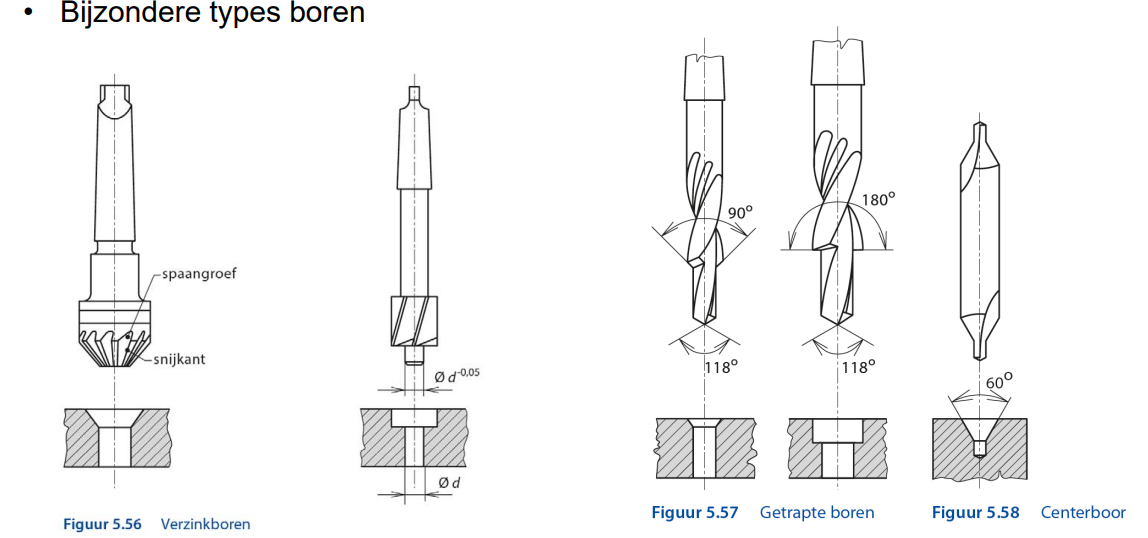
\includegraphics[width=1\textwidth]{assets/image44.png}
    \caption{Verschillende soorten boren}
\end{figure}

\subsection{Kotteren}
Als je een groot gat hebt en je kunt niet met een boor zo'n groot gat maken, dan kun je kotteren gebruiken.
Je kunt eventueel ook frezen, maar dat zie je in het volgende hoofdstuk~\ref{chap:Verspanen_Frezen}.
Bij kotteren laat je de beitel excentrisch meedraaien, waardoor je een grotere diameter uitverspaant
dan de kotterstang zelf.

\subsection{Draadtappen}
Draadtappen is het snijden van interne schroefdraad in een voorgeboord gat.

\begin{table}[ht]
    \centering
    \begin{tabularx}{0.8\textwidth}{|l|X|X|}
        \hline
        \textbf{Schroefdraad} & \textbf{Pitch (mm)} & \textbf{Tap‑boring (mm)} \\
        \hline
        M5~$\times$~0.8       & 0.8                 & 4.2                      \\
        \hline
        M6~$\times$~1.0       & 1.0                 & 5.0                      \\
        \hline
        M8~$\times$~1.25      & 1.25                & 6.75                     \\
        \hline
        M10~$\times$~1.5      & 1.5                 & 8.5                      \\
        \hline
    \end{tabularx}
    \caption{Veelvoorkomende metrische tap‑boringen}
\end{table}
\subsection{Ruimen}
Ruimen is een afwerkingsbewerking die een bestaand gat op nauwkeurige maat brengt met een goede oppervlaktekwaliteit.
De ruimer neemt slechts een dunne laag weg (enkele tienden van een millimeter) en volgt het bestaande gat,
zodat je maat en gladheid haalt die je met boren alleen niet bereikt (tot IT7).
\begin{figure}[ht]
    \centering
    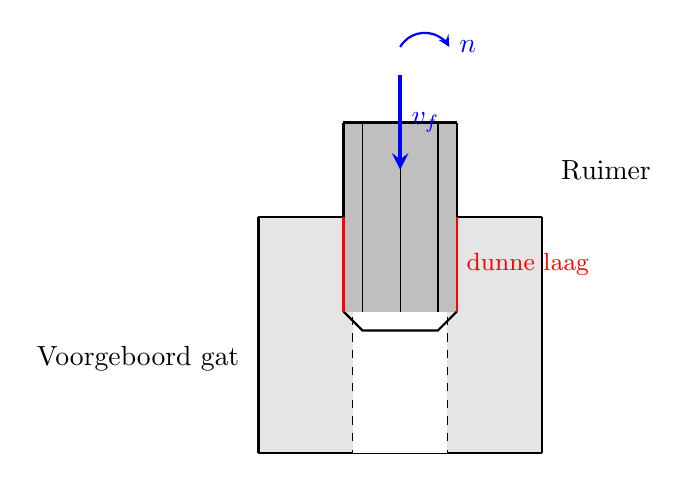
\begin{tikzpicture}[scale=1.2, >=stealth]
        % Werkstuk
        \fill[gray!20] (-1.5, 0) rectangle (1.5, -2.5);
        \draw[thick] (-1.5, 0) -- (1.5, 0);
        \draw[thick] (-1.5, -2.5) -- (1.5, -2.5);
        \draw[thick] (-1.5, 0) -- (-1.5, -2.5);
        \draw[thick] (1.5, 0) -- (1.5, -2.5);

        % Voorgeboord gat (iets kleiner dan de ruimer)
        \def\holeW{1.0}
        \fill[white] (-\holeW/2, 0) rectangle (\holeW/2, -2.5);
        \draw[dashed] (-\holeW/2, 0) -- (-\holeW/2, -2.5);
        \draw[dashed] (\holeW/2, 0) -- (\holeW/2, -2.5);

        % Ruimer (Reamer)
        \def\reamerW{1.2} % Iets breder dan het gat -> neemt materiaal af
        \def\reamerH{2.0}
        \begin{scope}[yshift=-1.0cm]
            \fill[gray!50] (-\reamerW/2, 0) rectangle (\reamerW/2, \reamerH);
            \draw[thick] (-\reamerW/2, 0) -- (-\reamerW/2, \reamerH);
            \draw[thick] (\reamerW/2, 0) -- (\reamerW/2, \reamerH);
            \draw[thick] (-\reamerW/2, \reamerH) -- (\reamerW/2, \reamerH);

            % Rechte tanden (Straight flutes)
            \draw[thin] (-0.4, 0) -- (-0.4, \reamerH);
            \draw[thin] (0, 0) -- (0, \reamerH);
            \draw[thin] (0.4, 0) -- (0.4, \reamerH);

            % Afgeschuinde onderkant (Chamfer)
            \draw[thick] (-\reamerW/2, 0) -- (-\reamerW/2 + 0.2, -0.2) -- (\reamerW/2 - 0.2, -0.2) -- (\reamerW/2, 0);
        \end{scope}

        % Materiaalafname indicatie
        \draw[red, thick] (-\reamerW/2, -1.0) -- (-\reamerW/2, 0);
        \draw[red, thick] (\reamerW/2, -1.0) -- (\reamerW/2, 0);
        \node[red, right] at (\reamerW/2, -0.5) {\small dunne laag};

        % Beweging
        \draw[->, ultra thick, blue] (0, 1.5) -- (0, 0.5) node[midway, right] {$v_f$};
        \draw[->, thick, blue] (0, 1.8) arc (150:30:0.3) node[right] {$n$};

        % Annotaties
        \node[right] at (1.6, 0.5) {Ruimer};
        \node[left] at (-1.6, -1.5) {Voorgeboord gat};

    \end{tikzpicture}
    \caption{Schematische weergave van ruimen: een ruimer verwijdert een dunne laag materiaal uit een voorgeboord gat voor hoge precisie en gladheid.}
\end{figure}
\FloatBarrier


\begin{warningbox}[EXAMEN CHECKLIST: BOREN]
    \begin{itemize}
        \item \textbf{Nauwkeurigheid}: Ken de haalbare IT-klassen voor boren, kotteren en ruimen.
        \item \textbf{Krachten}: Begrijp dat bij boren de voedingskracht $F_f$ dominant is (axiale penetratie).
        \item \textbf{Torsie}: Leg uit hoe de maximale voeding $f_{max}$ wordt beperkt door de torsiesterkte van de boor.
        \item \textbf{Gereedschap}: Ken de types (twist drill, reamer, countersink) en hun functie.
        \item \textbf{C-Frame}: Begrijp het effect van de machinebuiging op de haaksheid van het gat.
    \end{itemize}
\end{warningbox}

\chapter{Verspanen: Frezen}
\label{chap:Verspanen_Frezen}

Frezen is een verspaningstechniek waarbij een roterend snijgereedschap, de frees, wordt gebruikt om materiaal van een werkstuk te verwijderen.
Het proces omvat het bewegen van de frees langs het oppervlak van het werkstuk om de gewenste vorm of maat te bereiken.

\begin{description}
    \item[Hoofdbeweging] Je gereedschap, de \textbf{frees}, roteert.
    \item[Voedingsbeweging] Het gereedschap of het werkstuk schuift op om materiaal te verwijderen.
\end{description}

\section{Soorten frezen}
Snijd je met de \textbf{omtrek} (de mantel) van de frees, dan spreken we van \textbf{mantelfrezen}:
de freesas ligt evenwijdig met het bewerkte vlak.

Snijd je met de \textbf{kopse kant} (het eindvlak) van de frees, dan is dat \textbf{kopfrezen}:
de freesas staat loodrecht op het bewerkte vlak.

\section{Geometrie van de frees}

Net zoals bij draaien en boren zijn er verschillende vlakken op de frees die verschillende functies hebben.
\begin{itemize}
    \item \textbf{Spaangroef}
    \item \textbf{Vrijloophoek}
    \item \textbf{Snijkant}
    \item \textbf{Snijvlak}
    \item \textbf{Wighoek}
\end{itemize}

Deze hebben dezelfde eigenschappen als bij boren en draaien.
Je kunt meer info vinden bij Algemeen verspanen~\ref{chap:Algemeen verspanen}.

\begin{figure}[ht]
    \centering
    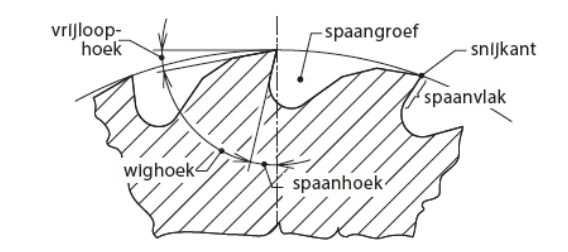
\includegraphics[width=0.6\textwidth]{assets/image45.png}
    \caption{Geometrie van een mantelfrees}
\end{figure}
\FloatBarrier


\section{Krachtwerking bij frezen}

Net zoals bij draaien en boren zijn er verschillende krachten die op het werkstuk
en de frees werken tijdens het frezen.
Ze worden met de theorie van Kienzle berekend.

\begin{wrapfigure}[16]{r}{0.55\textwidth}
    \centering
    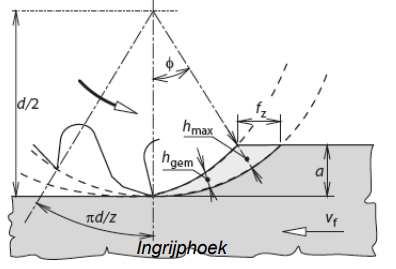
\includegraphics[width=\linewidth]{assets/image46.png}
    \caption{Krachten op een frees}
    \label{fig:frees_krachten}
\end{wrapfigure}
\FloatBarrier

De krachten op de frees zijn voornamelijk de snijkracht $F_c$ en de voedingskracht $F_f$; de terugdrukkracht $F_p$ is meestal kleiner en minder kritisch.
Een goed begrip van deze krachten is essentieel voor het optimaliseren van snijparameters en het waarborgen van gereedschapslevensduur.
\begin{itemize}
    \item \textbf{Snijkracht $F_c$:} hoofdkracht die het snijproces aandrijft.
    \item \textbf{Voedingskracht $F_f$:} kracht die de voeding van de frees aandrijft.
    \item \textbf{Terugdrukkracht $F_p$}: kracht loodrecht op $F_c$ en $F_f$, meestal kleiner.
\end{itemize}

De snededikte is niet constant omdat je frees ronddraait. Voor berekeningen wordt de gemiddelde snededikte gebruikt.
\newline

\belangrijk{BELANGRIJK VOOR EXAMEN}\\
De krachten op je frees zijn dus \emph{niet} constant: elke tand snijdt maar over een deel van de omwenteling,
en de snededikte varieert binnen die snede. Zorg dat je dit weet voor het examen.
Daarom rekenen we met de \textbf{gemiddelde snededikte} $h_{gem}$, zodat we toch één kracht kunnen berekenen.

\textbf{Gemiddelde snededikte bij Frezen:} $h_{gem} = f_z \cdot \sqrt{\dfrac{a}{d}}$\\
waarbij $f_z$ de voeding per tand is, $a$ de snedediepte en $d$ de diameter van de frees.

\textbf{Voeding per tand bij Frezen:} $f_z = \dfrac{f}{z_i}$
waarbij $f$ de voeding is en $z_i$ het aantal tanden van de frees.

\textbf{Snijsnelheid bij frezen:} $v_c = \dfrac{\pi \cdot d \cdot n}{1000}$
waarbij $v_c$ de snijsnelheid is [\si{m/min}], $d$ de diameter van de frees [\si{mm}] en $n$ het toerental [omw/min].

\textbf{Ingrijpingshoek bij Frezen:} $\displaystyle \phi = \arccos\!\left(1 - \dfrac{2a}{d}\right) \;\Rightarrow\; \cos\phi = 1 - \dfrac{2a}{d}$.
waarbij $a$ de snedediepte is en $d$ de diameter van de frees.

\textbf{Tanden in de snede:} $z_i = \dfrac{\phi}{360^\circ}\cdot z$
waarbij $z_i$ het aantal tanden is dat gelijktijdig in de snede zit,
$\phi$ de ingrijpingshoek in graden en $z$ het totale aantal tanden van de frees.


\frm{Snijkracht bij Frezen}{F_c = k_c \cdot b \cdot h_{gem}^{(1-e)} \cdot z_i}
{waarbij $F_c$ de snijkracht is [\si{N}], $k_c$ de snijkrachtcoëfficiënt [\si{N/mm^2}], $b$ de snedebreedte [\si{mm}], $h_{gem}$
de gemiddelde snededikte [\si{mm}], $z_i$ het aantal tanden in de snede [-] en $e$ de snijkrachtexponent [-].}

\frm{Snijmoment bij Frezen}{M_c = C_m \cdot d^{x_M} \cdot f_z^{y_M} \cdot z_i}
{waarbij $M_c$ het snijmoment is [\si{N.mm}], $C_m$ de momentcoëfficiënt [-], $d$ de diameter [\si{mm}], $f_z$ de voeding per tand
    [\si{mm/tand}], $z_i$ het aantal tanden in de snede [-] en $x_M, y_M$ de momentexponenten [-].}

\frm{Voedingskracht bij Frezen}{F_f = k_f \cdot b \cdot h_{gem}^{(1-e)} \cdot z_i}
{waarbij $F_f$ de voedingskracht is [\si{N}], $k_f$ de voedingskrachtcoëfficiënt [\si{N/mm^2}], $b$ de snedebreedte [\si{mm}],
$h_{gem}$ de gemiddelde snededikte [\si{mm}], $z_i$ het aantal tanden in de snede [-] en $e$ de voedingskrachtexponent [-].}

Bij frezen zijn de krachten op je frees niet constant.
De kracht op één tand per draaiing is parabolisch en als je de invloed van alle tanden samentelt krijg je een heuvelachtige
krachtcurve.
\begin{figure}[ht]
    \centering
    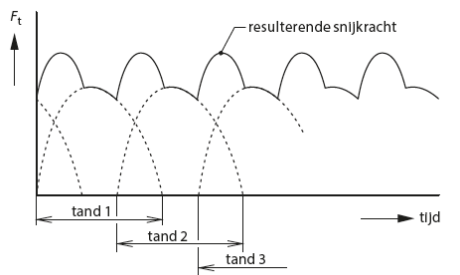
\includegraphics[width=0.5\textwidth]{assets/47.png}
    \caption{Krachtcurve bij frezen}
\end{figure}

\section{Richting van frezen}
Er zijn twee richtingen van frezen:
\begin{itemize}
    \item \textbf{Meelopend frezen}: De frees draait in dezelfde richting als de voeding. Dit zorgt voor een betere oppervlaktekwaliteit en minder gereedschapsbelasting.
    \item \textbf{Tegenlopend frezen}: De frees draait in de tegenovergestelde richting van de voeding. Dit kan leiden tot een ruwer oppervlak en hogere gereedschapsbelasting.
\end{itemize}

\begin{figure}[ht]
    \centering
    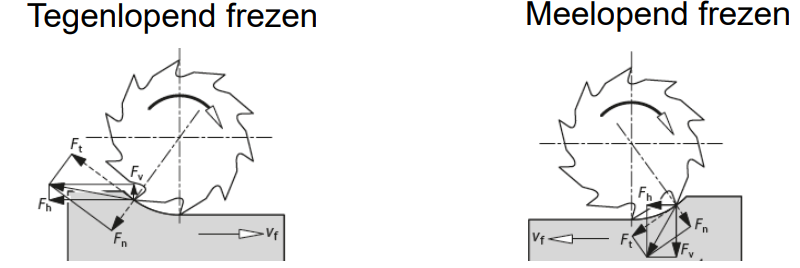
\includegraphics[width=1\textwidth]{assets/image48.png}
    \caption{Tegenlopend en meelopend frezen en de krachten die ze creëren}
    \label{fig:meelopend_tegenlopend}
\end{figure}

$v_f$ is de richting waarin het werkstuk beweegt (de voedingsrichting).

\begin{engtable}[
        caption = {Vergelijking: Tegenlopend vs Meelopend frezen},
        label = {tab:meelopend_vs_tegenlopend},
    ]{
        colspec = {l X X},
        width = \textwidth,
        cells = {font=\small},
        row{1} = {font=\bfseries},
    }
    Kenmerk & Tegenlopend & Meelopend \\
    Aandrijving & De horizontale krachtcomponent drukt het werkstuk weg van de frees. & De horizontale krachtcomponent trekt het werkstuk naar de frees toe. \\
    Speling & Geen compensatie nodig, veiliger bij backlash. & Spelingcompensatie onmisbaar. \\
    Spaanvorming & Dun $\rightarrow$ dik (de spaan groeit tijdens de snede). & Dik $\rightarrow$ dun (de spaan neemt af richting het einde). \\
    Snijkracht & Stijgt geleidelijk tijdens ingreep. & Stijgt sneller; hogere piekbelasting. \\
    Snijgedrag & Eerst wrijving, later snijden (meer smearing). & Meteen snijden (scherpere insnijding). \\
    Oppervlakte & Meestal matig. & Meestal beter (glad). \\
    Stabiliteit & Neiging tot klapperen / chatter. & Werkstuk wordt 'in klem' getrokken. \\
    Precisie & Minder voorspelbaar. & Kan preciezer zijn. \\
\end{engtable}
\FloatBarrier

\subsection{Wanneer kiezen: meelopend vs tegenlopend}
\textbf{Praktische richtlijnen:}
\begin{itemize}
    \item \textbf{Meelopend (climb milling)} -- kies dit bij een stijve machine en goede opspanning,
          vooral voor afwerking. De spaandikte neemt af tijdens de ingreep (dik $\rightarrow$ dun), er is minder wrijving bij de instap en doorgaans
          een betere oppervlaktekwaliteit en langere gereedschapslevensduur; vereist minimale backlash in de aandrijving.
    \item \textbf{Tegenlopend (conventional milling)} -- kies dit bij oudere of minder stijve machines,
          bij ruwe bewerkingen of wanneer er speling is. De spaandikte neemt toe tijdens de ingreep (dun $\rightarrow$ dik),
          bij de instap is er meer wrijving en kans op BUE, maar de methode is vaak veiliger voor onstabiele opstellingen of dunwandige onderdelen.
\end{itemize}

\paragraph{Effecten op oppervlakte en snedediepte}
\begin{itemize}
    \item \textbf{Oppervlaktekwaliteit:} Meelopend geeft doorgaans een gladdere afwerking.
          Tegenlopend geeft meer wrijving bij instap en vaak een ruwere afwerking.
    \item \textbf{Snedediepte/productiviteit:} In een stijve opstelling maakt meelopend vaak hogere snededieptes en hogere voedingen mogelijk zonder kwaliteitsverlies.
          Tegenlopend wordt vaak gebruikt voor grove, hoge‑volume snedes of wanneer de machine/opstelling de voorkeur geeft aan een voorzichtige instap.
\end{itemize}

\section{Soorten frezen}
\begin{itemize}
    \item \textbf{Mantelfrezen}: Hierbij wordt de omtrek (zijkant) van de frees gebruikt. Geschikt voor sleuven, contouren en zijvlakken.
    \item \textbf{Kopfrezen}: Hierbij wordt de kopse kant van de frees gebruikt. Geschikt voor het vlakken van grote oppervlakken; per snede wordt een grote breedte bestreken.
    \item \textbf{Bolfrezen}: Hierbij wordt een frees met een bolvormige snijkant gebruikt, geschikt voor het maken van gebogen oppervlakken en complexe 3D-vormen.
    \item \textbf{Vormfrezen}: Hierbij wordt een frees met een specifieke vorm gebruikt om profielen en vormen in het materiaal te frezen.
    \item \textbf{Circulair frezen}: Hierbij wordt een cirkelvormige beweging gebruikt om gaten of cirkelvormige uitsparingen te maken.
    \item \textbf{Brootsen (trekruimen)}: Hierbij wordt een getrapt gereedschap in één rechtlijnige beweging door of langs het werkstuk getrokken; elke tand neemt iets meer weg. Zeer nauwkeurig en snel, maar het gereedschap is duur en productspecifiek (bv.\ spiebanen, inwendige vertandingen).
\end{itemize}

\section{De Freesmachine}
Een freesmachine heeft een tafel waarop je werkstuk wordt geklemd. In de spindel steek je de mantel- of kopfrees.
De frees roteert en de tafel beweegt in de $x$-, $y$- en $z$-richting.


\begin{figure}[htbp]
    \centering
    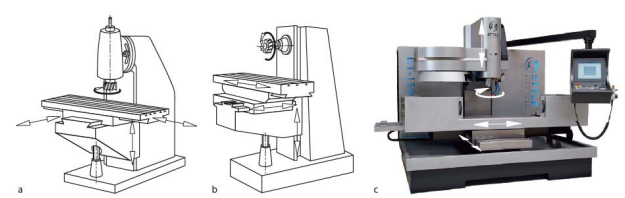
\includegraphics[width=0.8\textwidth]{assets/image49.png}
    \caption{Weergave van een freesmachine}
\end{figure}
\vspace{2cm}

\begin{warningbox}[EXAMEN CHECKLIST: FREZEN]
    \begin{itemize}
        \item \textbf{Krachten}: Begrijp dat snijkrachten bij frezen variëren (heuvelachtig verloop) en dat we $h_{gem}$ gebruiken voor berekeningen.
        \item \textbf{Richting}: Ken het cruciale verschil tussen \keyterm{meelopend} (spaan dik $\to$ dun) en \keyterm{tegenlopend} (spaan dun $\to$ dik) frezen.
        \item \textbf{Geometrie}: Weet wat de ingrijpingshoek $\phi$ is en hoe die de belasting van de tanden bepaalt.
        \item \textbf{Technieken}: Onderscheid mantelfrezen (omtrek) en kopfrezen (kopse kant).
    \end{itemize}
\end{warningbox}

\chapter{Verspanen: Hybridetechnieken}

\section{Honen}

\begin{conceptbox}[Honen]
    Honen is een nabewerkingsproces voor cilindrische oppervlakken (zoals motorcilinders)
    om de nauwkeurigheid (IT3-IT5) en de oppervlaktekwaliteit te krijgen.
    De bewerking combineert een roterende en een axiaal oscillerende beweging, wat een karakteristiek kruispatroon achterlaat.
\end{conceptbox}

Honen is een slijpoperatie die twee bewegingen combineert: een rotatie en een heen-en-weergaande beweging.
\begin{description}
    \item[Hoofdbeweging] Bij honen is de hoofdbeweging een rotatie van de hoonkop.
    \item[Voedingsbeweging] De axiale heen-en-weergaande beweging waarmee het gereedschap
          langs het oppervlak schuift, plus de radiale aanzet van de hoonstenen.
    \item[Kruispatroon] Doordat rotatie en axiale slag samenvallen, laten de stenen elkaar kruisende krassen na.
          Dat kruispatroon houdt olie vast, wat precies de bedoeling is in een motorcilinder.
\end{description}
Honen brengt de nauwkeurigheid tot IT3.

\subsection{Lange-slag Honen}
\vspace{0.5cm}

\begin{figure}[htbp]
    \centering
    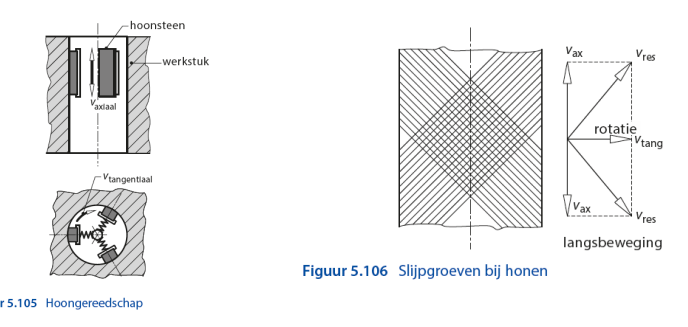
\includegraphics[width=0.8\textwidth]{assets/image56.png}
    \caption{Lange-slag honen}
    \label{fig:lange-slag-honen.png}
\end{figure}

Een hoonsteen wordt gebruikt om het oppervlakte van een cilinder te verbeteren.
De hoonsteen heeft een lange slag en beweegt heen en weer in de lengte van de cilinder.
Dit zorgt voor een betere oppervlaktekwaliteit en nauwkeurigheid van de cilinder.

Bij het honen neem je enkel de \emph{toppen} van de oppervlakteruwheid weg; de dalen blijven staan.
Dat is anders dan bij slijpen, waar de hele laag wordt afgenomen en er toch nog een licht golvend oppervlak kan achterblijven.

% --- Illustratie: ruw oppervlak en resultaat na honen (scherpe toppen, geclipt) ---
\begin{figure}[htbp]
    \centering
    \makebox[\textwidth][c]{%
        \begin{tikzpicture}[x=0.85cm, y=2.2cm, >=Stealth, every node/.style={font=\small}]
            % Parameters
            \def\L{5.8} % totale lengte
            \def\cut{0.45} % hoogte van de snijlijn (y-waarde)

            % --- (a) Voorbehandeld oppervlak ---
            \begin{scope}[shift={(0,0)}]
                % Basislijn
                \draw[black!40, thick] (0,0) -- (\L,0);

                % De toppen tekenen en de oranje delen inkleuren
                % Formaat: x-positie / hoogte
                \foreach \x/\h in {0.4/0.95, 1.2/1.05, 2.0/0.9, 2.8/1.1, 3.6/0.8, 4.4/1.0, 5.2/0.88} {
                        % Teken de driehoek (contour)
                        \draw[very thick, black] (\x-0.4, 0) -- (\x, \h) -- (\x+0.4, 0);

                        % Bereken de snijpunten voor het oranje driehoekje (lineaire interpolatie)
                        % x_breedte_op_snijlijn = 0.4 * (1 - cut/h)
                        \pgfmathsetmacro{\xoffset}{0.4 * (1 - \cut/\h)}
                        \fill[orange, opacity=0.55] (\x-\xoffset, \cut) -- (\x, \h) -- (\x+\xoffset, \cut) -- cycle;
                    }

                % Snijlijn
                \draw[very thick, red] (-0.2, \cut) -- (\L+0.2, \cut) node[right, black]{\textbf{snijlijn}};

                % Label
                \node[below] at (\L/2, -0.2) {(a) Voorbehandeld oppervlak};
            \end{scope}

            % --- Hoonproces pijl ---
            \draw[->, very thick] (6.0, 1.0) -- (6.8, 1.0);
            \node[above, font=\bfseries] at (6.4, 1.05) {HOONPROCES};

            % --- (b) Gehoond oppervlak (Trapezoïdes) ---
            \begin{scope}[shift={(7.5,0)}]
                \draw[black!40, thick] (0,0) -- (\L,0);

                \foreach \x/\h in {0.4/0.95, 1.2/1.05, 2.0/0.9, 2.8/1.1, 3.6/0.8, 4.4/1.0, 5.2/0.88} {
                        % Bereken de breedte van de platte top op de snijlijn
                        \pgfmathsetmacro{\xoffset}{0.4 * (1 - \cut/\h)}

                        % Teken de trapezoïde (het restant onder de snijlijn)
                        \draw[very thick, black, fill=gray!15]
                        (\x-0.4, 0) -- (\x-\xoffset, \cut) -- (\x+\xoffset, \cut) -- (\x+0.4, 0) -- cycle;
                    }

                % Snijlijn
                \draw[very thick, red] (-0.2, \cut) -- (\L+0.2, \cut);

                % Label
                \node[below] at (\L/2, -0.2) {(b) Gehoond oppervlak};
            \end{scope}

            % --- Legende ---
            \begin{scope}[shift={(3.5, -1.0)}]
                \draw[very thick, red] (0, 0.4) -- (0.8, 0.4) node[right=5pt, black] {Snijlijn};
                \fill[orange, opacity=0.55] (0, 0) rectangle (0.8, 0.25);
                \node[right=5pt] at (0.8, 0.125) {Te verwijderen toppen (gemarkeerd)};
            \end{scope}

        \end{tikzpicture}
    }

    \caption{(a) Voorbehandeld, ruw oppervlak met scherpe toppen; (b) resultaat na honen waarbij de
        bovenste delen van de toppen zijn verwijderd.}
    \label{fig:hoonprocess_schematic}
\end{figure}
\vspace{0.35cm}

\subsection{Korte-slag Honen}
\vspace{0.25cm}
Het enige verschil met lange-slag honen is de kinematica van het systeem.
Je werkstuk is opgespannen tussen twee tegenpunten die het laten roteren.
De hoonsteen wordt daarbij van buitenaf op het oppervlak gedrukt.
Je past de hoonsteen hier dus toe op een \emph{uitwendig} cilindrisch oppervlak, zoals bij het nabewerken van zuigerstangen.
De steen maakt een sinusoïdale beweging met een korte slag.
De oppervlaktekwaliteit is enorm fijn.

\begin{figure}[htbp]
    \centering
    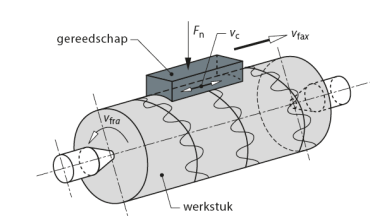
\includegraphics[width=0.5\textwidth]{assets/image57.png}
    \caption{Kortslag honen van een werkstuk}
    \label{fig:kortslag-honen.png}
\end{figure}
\FloatBarrier

\section{Leppen}
Bij het leppen gebruik je enorm fijne, \emph{vrije} korrels die in een pasta, olie of gel zitten.
De werkstukken zitten in een houder of vat en worden daarin bewogen.

\subsection{Met vloeistof}
De lepvloeistof met de korrels beweegt tussen de stukken en maakt het oppervlak enorm fijn.
Tot en met $R_a = \SI{0,1}{\micro m}$ en IT1 is mogelijk.

\textbf{Toepassingen}:
\newline
Bepaalde stukken hebben dit nodig, zoals kogellagers of klepzittingen.

\textit{Kijk zeker de video's op Toledo om dit proces beter te begrijpen.}

\subsection{Finisheren met pasta}
Je klemt het werkstuk in en pompt dan de pasta met korrels erdoor om het oppervlak te verbeteren.

\section{Geavanceerde verspaningstechnieken en hybride technieken}

\subsection{Hoge snelheid verspanen}
Bij hogesnelheidsverspanen (HSM) gebruik je enorm hoge snijsnelheden in vergelijking met
conventioneel verspanen.
\newline
\begin{figure}[ht]
    \centering
    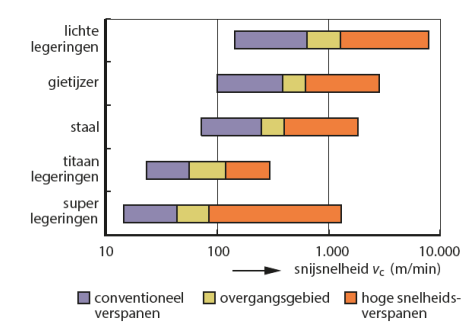
\includegraphics[width=0.8\textwidth]{assets/image58.png}
    \caption{Hoge snelheid verspanen in vergelijking met conventioneel verspanen}
    \label{fig:hoge_snelheid_verspanen.png}
\end{figure}

Deze spindels gaan tot 20.000 à 30.000 omw/min, afhankelijk van het materiaal dat je verspaant.

Herinner je bij algemeen verspanen~\ref{chap:Algemeen verspanen} dat bij heel hoge
snijsnelheden je een \textbf{Softening effect} had die het makkelijker maakte om te verspanen.
Je werkmateriaal wordt warmer en daarom ductieler.

Bij hogesnelheidsverspanen zie je dit effect ook terugkomen.
De warmte die gegenereerd wordt, gaat grotendeels mee in de spaan: die wordt zo snel afgevoerd dat de
warmte niet de tijd krijgt om in het werkstuk te diffunderen en het oppervlak aan te tasten.
\textit{Dit effect ken je al uit figuur~\ref{verschillende_invloeden_voeding_snedediepte}.}

\textbf{Toepassingen:}
\newline
Je wilt enorm snel materiaal wegnemen.
Je zet dus je voeding $f$ en je snijsnelheid $v_c$ enorm hoog.
Deze techniek wordt vooral gebruikt bij aluminium en andere lichte metalen.
\newline
De gereedschappen zijn van (gecoat) hardmetaal: hard genoeg om hun snijkant te behouden bij de
hoge temperaturen die daarbij optreden.


\subsection{Hardverspanen}

\begin{conceptbox}[Hardverspanen]
    Hardverspanen is het direct draaien of frezen van geharde materialen ($>45$ HRC) die voorheen enkel geslepen konden worden. Dit vereist extreem stijve machines en gereedschappen zoals PCBN (Polycrystalline Cubic Boron Nitride).
\end{conceptbox}

Hardverspanen is het verspanen van harde materialen zoals gehard staal, keramiek en andere harde legeringen.
De ontwikkeling van hoge snelheidsfrezen en veel stevigere machines maakte dit mogelijk.

Je moet een negatieve spaanhoek $\gamma$ gebruiken die meer kracht vraagt omdat de
afschuifhoek $\phi$ kleiner wordt.
Als compensatie gebruik je kleine snededieptes om de krachten te beperken.

Nieuwe, harde beitels en stijve machines die de hoge krachten aankunnen, maken hardverspanen
op een aanvaardbare tijd mogelijk. Zo vervangt het in veel gevallen het veel tragere slijpen.

\section{Hybrideprocessen}
Hybride processen vormen een ruim domein waarbij je verschillende technieken combineert om
werkstukken te bewerken.
Je gaat dus twee technieken toepassen om bijvoorbeeld dingen makkelijker te verspanen
of om betere oppervlaktekwaliteit te krijgen.

Dit zijn vooral experimentele technieken die nog in ontwikkeling zijn.

\subsection{Laserondersteuning bij verspanen}
Je warmt het materiaal vlak voor de beitel op met een laser. Het oppervlak wordt warmer
en dus ductieler, waardoor het makkelijker te verspanen is.

Het is energie-efficiënt: de laser kost energie, maar het warmere materiaal vraagt zoveel minder
snijkracht dat je er netto op wint (en je gereedschap gaat langer mee).

\begin{figure}[ht]
    \centering
    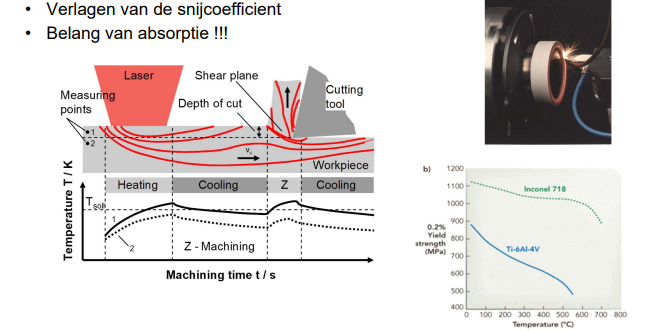
\includegraphics[width=1\textwidth]{assets/image59.png}
    \caption{Laserondersteuning bij verspanen}
    \label{fig:laserondersteuning-bij-verspanen.png}
\end{figure}
\FloatBarrier

Het materiaal moet het laserlicht wel goed \emph{absorberen}.
Je wilt zo weinig mogelijk reflectie en transmissie.

\frm{Energiebalans van licht op een materiaal}
{1 = A + R + T}{waarbij $A$ de absorptie is [-], $R$ de reflectie [-] en $T$ de transmissie [-].
    Alle drie zijn fracties van het invallende vermogen, dus ze tellen altijd op tot 1.}
\vspace{0.5cm}

\subsection{Draadvonken en slijpen}
\textit{(je ziet meer over draadvonken in een ander hoofdstuk)}
Het vonkproces is een thermisch proces: je neemt eerst materiaal weg met vonken.
Bij normaal draadvonken blijft er een laagje hergestold materiaal (de witte laag) op het oppervlak achter;
door daarna te slijpen neem je die laag weg.

\subsection{ECM (Electro Chemical Machining) en slijpen}
Bij ECM ga je materiaal wegnemen door elektrochemische reacties.
Je hebt een anode en kathode die in een elektrolyt zitten.
Dit chemische proces laat een ruw oppervlak en oxidelagen achter.
Door daarna te slijpen verbeter je dat oppervlak en verwijder je die laag.

\subsection{Combinatie van ECM en frezen}
Je gaat frezen combineren met ECM.
De chemische bewerkingen laten een oxidelaag achter die je met frezen gaat verwijderen.

\textit{(Deze technieken zijn niet super belangrijk om vanbuiten te kennen maar je moet zien dat je nadelen van een proces kunt oplossen met een ander proces)}

\begin{warningbox}[EXAMEN CHECKLIST: HYBRIDETECHNIEKEN]
    \begin{itemize}
        \item \textbf{Honen}: Weet dat dit dient voor het verwijderen van toppen in cilinders (IT3-IT5).
        \item \textbf{Leppen}: Begrijp dat dit werkt met vrije korrels in een pasta voor extreme gladheid (IT1).
        \item \textbf{Hoge Snelheid Verspanen (HSM)}: Leg uit waarom de warmte bij HSM grotendeels in de spaan gaat (Softening effect).
        \item \textbf{Hardverspanen}: Ken de noodzaak voor negatieve spaanhoeken en stijve machines.
        \item \textbf{Hybride Concept}: Begrijp hoe lasers of ECM kunnen helpen om krachten te verlagen of oppervlakken te finishen.
    \end{itemize}
\end{warningbox}

\chapter{Verspanen: Slijpen}

\begin{conceptbox}[Onbepaalde snijkant]
    In tegenstelling tot draaien of frezen, heeft slijpen geen vaste snijkantgeometrie. Het oppervlak van de slijpsteen bestaat uit ontelbare, willekeurig georiënteerde korrels die materiaal afnemen met een sterk negatieve spaanhoek.
\end{conceptbox}

Slijpen is een verspaningstechniek waarbij een roterend schijfvormig gereedschap,
de slijpschijf, wordt gebruikt om materiaal van een werkstuk te verwijderen.
Het verspanen gebeurt door een slijpsteen waarvan de \textbf{snijkorrels} kleine deeltjes materiaal van het werkstuk afnemen.
De korrels liggen willekeurig georiënteerd, dus de snijgeometrie ligt niet vast: we spreken van een \emph{onbepaalde} snijkant.

De snijkorrels kunnen oftewel vrij liggen of gebonden zijn in een matrix.

\textbf{Vrije snijkorrels:} losse korrels die losjes op het werkstuk inwerken of in suspensie of pasta. Voorbeelden:
\begin{itemize}
    \item \textbf{Leppen}: korrels in een pasta om zeer nauwkeurige oppervlakken te verkrijgen.
    \item \textbf{Stralen}: korrels in een straal om vuil of roest te verwijderen.
\end{itemize}
Je stuurt de korrels dus langs het werkstuk om de oppervlaktekwaliteit te verbeteren.

Korrels kunnen ook gebonden zijn in een matrix.

\textbf{Gebonden snijkorrels:} korrels die vastzitten in een matrixmateriaal. Voorbeelden:
\begin{itemize}
    \item \textbf{Slijpschijven}: korrels gebonden in een harde matrix voor het slijpen van metalen.
    \item \textbf{Schuurpapier}: korrels gebonden op papier of stof voor handmatig schuren.
    \item \textbf{Honen}: korrels gebonden in een zachte matrix voor het verbeteren van de oppervlakteafwerking en nauwkeurigheid van gaten.
\end{itemize}


\section{Slijpen als frezen met onbepaalde snijkanten}
Bij slijpen heeft elke korrel een sterk \textbf{negatieve spaanhoek}, wat het verspanen op zich moeilijker maakt:
de kracht \emph{per volume-eenheid} afgenomen materiaal ligt veel hoger dan bij frezen.
Maar de \textbf{snedediepte} per korrel is zó klein (micrometers) dat de kracht per korrel toch beperkt blijft.
Die twee compenseren elkaar.

Je kunt een slijpsteen dus zien als een frees met heel veel, heel kleine, onbepaalde snijkanten.
\newline

\begin{figure}[htbp]
    \centering
    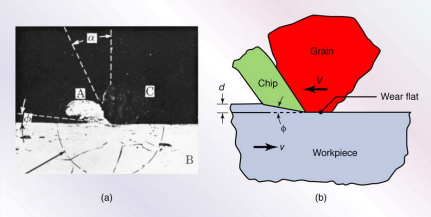
\includegraphics[width=0.6\textwidth]{assets/image50.png}
    \caption{Spaanvorming bij slijpen}
    \label{Spaanvorming bij slijpen}
\end{figure}

De korrel hier heeft een enorm negatieve spaanhoek. De spaanvorming is enorm klein maar omdat de korrels
zo klein en hard zijn kun je zelfs heel harde materialen slijpen.
\newline
\section{Eigenschappen van slijpen}
\begin{enumerate}
    \item \textbf{Snijsnelheid $v_c$}: ongeveer 25 tot 60 m/s, dus heel hoge snelheden (vergelijk: draaien zit rond 1--5 m/s).
    \item \textbf{Krachten $F_c$}: De krachten zijn hoog door de negatieve spaanhoek en omdat je harde materialen kunt slijpen.
    \item \textbf{Warmteontwikkeling}: Veel energie gaat verloren als warmte, slijpen kan aan het oppervlakte een temperatuur van \textbf{800 tot 900°C} veroorzaken.
          Dit kan leiden tot thermische beschadiging van het werkstuk. Je hebt dus materiaalveranderingen aan het oppervlakte.
          Intensieve koeling is dus nodig.
    \item \textbf{Snedediepte $a$}: Zeer kleine snededieptes, typisch in de orde van micrometers.
    \item \textbf{Slijtage van de slijpkorrel}: Slijpkorrels worden bot en vallen er dan af.
          Je moet de slijpschijf dus regelmatig terug scherp en op maat brengen door een laagje van het
          steenoppervlak af te nemen. Dat noemen we \textbf{dresseren} (dressing).
    \item \textbf{Oppervlaktekwaliteit}: Slijpen kan zeer fijne oppervlakteafwerkingen bereiken, vaak in de orde van enkele micrometers $R_a$.
    \item \textbf{Nauwkeurigheid}: Slijpen gebeurt op machines die enorm stijf zijn en dus nauwelijks meegeven tijdens het slijpen.
          Hierdoor kun je zeer nauwkeurige afmetingen bereiken.
    \item \textbf{Toepassingen}: Slijpen kan toegepast worden op zeer harde materialen zoals gehard staal en keramiek.
\end{enumerate}

\section{Parameters slijpsteen}

Een slijpsteen wordt gekarakteriseerd door vijf eigenschappen:
\begin{enumerate}
    \item \textbf{Korrelmateriaal}: waaruit de korrels zelf bestaan (korund, siliciumcarbide, CBN, diamant).
    \item \textbf{Korrelgrootte}: grotere korrels verwijderen sneller materiaal maar geven een ruwere afwerking;
          kleinere korrels geven een fijnere afwerking.
    \item \textbf{Hardheid van de slijpsteen}: hoe stevig het bindmiddel de korrels vasthoudt. Een ``harde'' steen
          houdt de korrels lang vast, een ``zachte'' laat ze sneller los.
    \item \textbf{Bindmiddel}: het materiaal dat de korrels bij elkaar houdt (keramisch, kunsthars, metaal, rubber).
    \item \textbf{Structuur}: het volumeaandeel poriën tussen de korrels, waar de spanen in kunnen.
\end{enumerate}

\begin{figure}[ht]
    \centering
    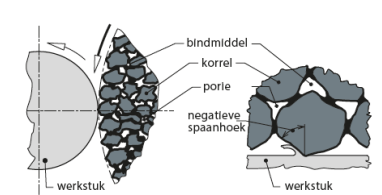
\includegraphics[width=0.6\textwidth]{assets/image51.png}
    \caption{Doorsnede van een slijpschijf}
    \label{fig:slijpsteen doorsnede.png}
\end{figure}
\subsection{Korrelmateriaal}
\textbf{Natuurlijke korrels} zijn kwarts, korund en (natuurlijk) diamant.
\newline
\textbf{Kunstmatige korrels} zijn siliciumcarbide, aluminiumoxide, kubisch boornitride (CBN) en synthetisch diamant.
\subsection{Korrelgrootte}
De korrelgrootte bepaalt hoeveel je kunt afnemen.
Grote korrels $\to$ meer afname, maar slechtere oppervlaktekwaliteit.
Kleine korrels $\to$ minder afname, maar betere oppervlaktekwaliteit.
\newline
De korrelgrootte wordt aangegeven met een \emph{meshnummer}: het aantal mazen per inch van de zeef
waarmee de korrels gesorteerd worden. Een hoger meshnummer betekent dus \emph{fijnere} korrels.

\section{Hardheid van de slijpsteen}

\begin{conceptbox}[Slijpverhouding (G-ratio)]
    De slijpverhouding $G$ wordt gedefinieerd als het volume verwijderd materiaal gedeeld door het volume verloren slijpsteen. Een hoge $G$-waarde duidt op een efficiënt proces waarbij weinig gereedschapsslijtage optreedt.
    \[ G = \frac{V_{verwijderd}}{V_{steen}} \]
\end{conceptbox}

De hardheid van een slijpsteen slaat niet op de hardheid van de korrels zelf, maar op hoe stevig het
bindmiddel ze vasthoudt. Ze wordt gemeten via de slijpverhouding:
\[G = \frac{\text{volume verspaand werkstukmateriaal}}{\text{volume verloren slijpschijf}}\]
Bij een grote $G$ neem je veel materiaal af tegenover weinig schijfverlies.
Bij een kleine $G$ verlies je veel slijpschijf voor weinig afname.

Bij een hard werkstukmateriaal moet je een \emph{zachte} slijpsteen gebruiken. Dat lijkt eerst tegenstrijdig,
maar bij harde materialen worden de korrels snel bot.
Je wilt dus dat botte korrels er vanzelf uitvallen zodat er nieuwe, scherpe korrels blootkomen.
Dat heet \textbf{zelfscherpend} gedrag: de steen dresseert zichzelf en je moet minder vaak manueel dresseren.
\subsection{Bindmiddel}
Het bindmiddel houdt de korrels bij elkaar.
Een paar voorbeelden zijn keramiek (klei), mineralen, metaal, kunsthars en elastische materialen.

Bij pastaslijpen gebruikt men bijvoorbeeld een elastisch bindmiddel, zodat de korrels zich naar het werkstuk
kunnen schikken. We spreken daar niet van een slijpverhouding $G$, omdat die daar niet relevant is.

\subsection{Structuur}
De structuur is de grootte van de poriën in verhouding tot het volumeaandeel bindmiddel en korrels.
Die poriën zijn de kleine openingen tussen de korrels, en ze zijn belangrijk: de spaantjes moeten erin passen.
Zitten ze vol, dan snijdt de steen niet meer en wrijft ze alleen nog (``dichtsmeren'').
De poriegrootte kies je dus afhankelijk van de bewerking en van de contacttijd tussen slijpschijf en werkstuk.

\textbf{Met al deze eigenschappen kun je een slijpsteen karakteriseren.}

\begin{examenbox}
    Weten dat alle factoren hieronder
    een slijpsteen karakteriseren:
\end{examenbox}

\begin{figure}[htbp]
    \centering
    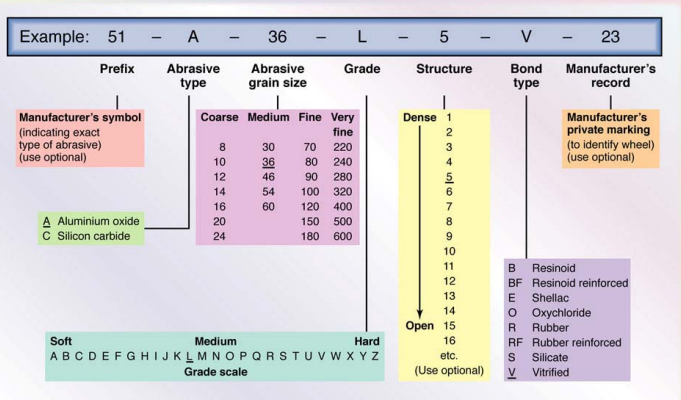
\includegraphics[width=0.6\textwidth]{assets/image52.png}
    \caption{}
    \label{fig:karateriseren van slijpsteen.png}
\end{figure}
\FloatBarrier

\section{Temperaturen bij slijpen}

Ongeveer $70\%$ van de energie die je bij het slijpen inbrengt, komt als warmte in het werkstuk terecht.
Dit kan leiden tot thermische beschadiging van het werkstuk.
Je moet oppassen voor:
\begin{itemize}
    \item \textbf{Vonken}
    \item \textbf{Structuurveranderingen}
    \item \textbf{Verbranding}
    \item \textbf{Scheurtjes}
    \item \textbf{Residuële spanningen}
\end{itemize}

Je moet dus voldoende koelen of nog een laatste warmtebehandeling doen na het slijpen.
\begin{figure}[htbp]
    \centering
    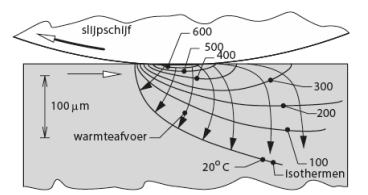
\includegraphics[width=0.5\textwidth]{assets/image53.png}
    \caption{Warmte bij Slijpen}
    \label{fig:warmte_bij_slijpen.png}
\end{figure}
\FloatBarrier

\section{Slijptechnieken}

\begin{wrapfigure}[13]{r}{0.6\textwidth}
    \centering
    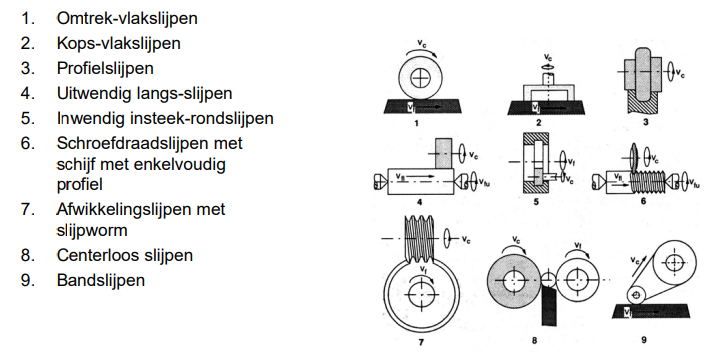
\includegraphics[width=\linewidth]{assets/image54.png}
    \caption{Alle soorten slijptechnieken}
    \label{fig:Slijptechnieken.png}
\end{wrapfigure}

Profielslijpen is slijpen van een bepaald profiel. Je slijpsteen heeft dus een gewenste vorm,
waar je het werkstuk mee slijpt.

Je kunt heel precieze tandwielen maken met profielslijpen: je slijpt de tandholtes met een slijpsteen
die exact de vorm van de tandholte heeft.

\textit{Tip: hier is hij niet veel op ingegaan.}


\section{De slijpmachine}
Slijpmachines zijn enorm stijf. Omdat je snedediepte maar enkele micrometers bedraagt, kan de kleinste
uitwijking of trilling ervoor zorgen dat je ineens niet meer snijdt, of net veel te diep gaat.
Je werkt dus in de orde van micrometers, en dan telt elke doorbuiging mee.

\subsection{Centerloos slijpen}
Centerloos slijpen is een slijptechniek waarbij het werkstuk niet wordt vastgehouden door een as of klem,
maar in plaats daarvan wordt ondersteund door twee rollen en aangedreven door een derde rol.
\begin{figure}[ht]
    \centering
    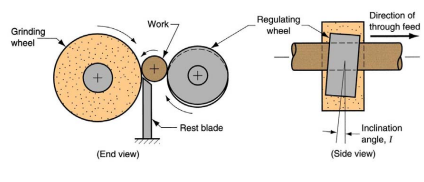
\includegraphics[width=0.8\textwidth]{assets/image55.png}
    \caption{Centerloos slijpen}
    \label{fig:centerloos_slijpen.png}
\end{figure}

\subsection{Profielslijpen}
Zoals hiervoor gezegd.
Je slijpt een bepaald profiel met een slijpsteen die dat profiel heeft.

\begin{warningbox}[EXAMEN CHECKLIST: SLIJPEN]
    \begin{itemize}
        \item \textbf{Onbepaalde snijkant}: Begrijp het verschil met gedefinieerde snijkanten en de impact van de negatieve spaanhoek.
        \item \textbf{Karakterisering}: Ken de 5 factoren: korrelmateriaal, korrelgrootte, hardheid, bindmiddel en structuur (porositeit).
        \item \textbf{Warmte}: Weet dat $70\%$ van de energie in warmte gaat ($900^\circ$C) en ken de risico's (TAZ, scheuren).
        \item \textbf{Dressing}: Leg uit waarom een slijpsteen regelmatig "gedressed" moet worden (scherp maken en profileren).
        \item \textbf{Centerloos slijpen}: Begrijp het principe en de voordelen voor massaproductie.
    \end{itemize}
\end{warningbox}

\chapter{Fysische, Chemische afnemende bewerkingen}

\section{Vonkerosie}

\begin{conceptbox}[EDM (Electro Discharge Machining)]
    EDM verwijdert materiaal door gecontroleerde elektrische ontladingen (vonken) tussen een elektrode en het werkstuk in een isolerend diëlektricum. Het proces is thermisch: materiaal wordt lokaal gesmolten en verdampt zonder mechanische krachten.
\end{conceptbox}

\textbf{EDM (Electro Discharge Machining)} of \textbf{vonkerosie} is een \textbf{verspaningstechniek} waarbij materiaal wordt
verwijderd door middel van \textbf{elektrische vonken}.
Je hebt een \textbf{elektrode} en een \textbf{werkstuk} die in een \textbf{vloeistof} (die als \textbf{isolator} fungeert zoals bijvoorbeeld gedestilleerd water) zitten.
Wanneer er een \textbf{hoge spanning} wordt aangelegd tussen de elektrode en het werkstuk, ontstaat
een elektrische vonk die het materiaal op het werkstuk smelt en wegneemt.
\newline
Je kunt geen normaal water gebruiken omdat er mineralen in zitten die wel geleiden.

\begin{figure}[htbp]
    \centering
    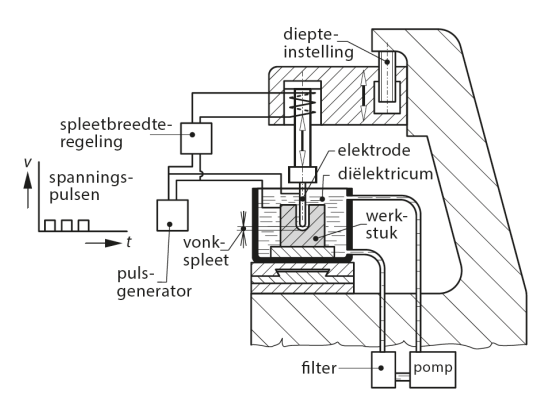
\includegraphics[width=0.5\textwidth]{assets/image60.png}
    \caption{Vonkerosie proces}
    \label{fig:vonkerosie_proces.png}
\end{figure}

\begin{figure}[htbp]
    \centering
    \begin{tikzpicture}
        \tikzset{
            elec/.style={fill=gray!30, draw=black, thick},
            work/.style={fill=gray!10, draw=black, thick, pattern=north east lines},
            spark/.style={decoration={zigzag, segment length=1mm, amplitude=0.5mm}, decorate, draw=orange, very thick},
            rough/.style={decorate, decoration={random steps, segment length=0.4mm, amplitude=0.2mm}}
        }

        % LEFT: BEFORE
        \begin{scope}[local bounding box=before]
            % Electrode (Top +)
            \draw[elec] (-0.5, 2.5) -- (-0.5, 1.5) -- (0, 0.5) -- (0.5, 1.5) -- (0.5, 2.5) -- cycle;
            \node at (0, 2) {$+$};

            % Workpiece (Bottom -)
            \draw[work] (-1.5, 0) rectangle (1.5, -1);
            \node[fill=white, inner sep=1pt] at (0, -0.5) {$-$};

            % Spark
            \draw[spark] (0, 0.5) -- (0, 0);
            % Text moved to the right with a pointer to the spark
            \node[right, font=\footnotesize, align=left] (lbl) at (0.6, 0.25) {\textbf{Warmtegeneratie}\\(vonk)};
            \draw[->, thin] (lbl.west) -- (0.1, 0.25);

            \node[below=0.2cm] at (0, -1) {\textbf{Voor}};
        \end{scope}

        % RIGHT: AFTER
        \begin{scope}[xshift=7cm, local bounding box=after]
            % Electrode (Top +)
            \draw[elec] (-0.5, 2.5) -- (-0.5, 1.5) -- (0, 0.5) -- (0.5, 1.5) -- (0.5, 2.5) -- cycle;
            \node at (0, 2) {$+$};

            % Workpiece (Bottom -) with ROUGH crater
            % Replaced smooth arc with a decorated path for roughness
            \draw[work] (-1.5, 0) -- (-0.4, 0)
            decorate[rough] { arc[start angle=180, end angle=360, radius=0.4] }
            -- (1.5, 0) -- (1.5, -1) -- (-1.5, -1) -- cycle;

            \node[fill=white, inner sep=1pt] at (0, -0.6) {$-$};

            \node[below=0.2cm] at (0, -1) {\textbf{Na}};
        \end{scope}

    \end{tikzpicture}
    \caption{Principe van vonkerosie: warmtegeneratie door elektrische ontlading zorgt voor materiaalafname (ruw oppervlak).}
    \label{fig:vonkerosie_principe}
\end{figure}
\FloatBarrier

\subsection{Componenten van een EDM-systeem}
Bij een vonkerosie-opstelling (zoals in \cref{fig:vonkerosie_proces.png}) zijn de volgende componenten cruciaal:
\begin{itemize}
    \item \textbf{Pulsgenerator}: De energiebron die hoogfrequente DC-pulsen levert. Hij regelt de aan-tijd ($t_{on}$) en uit-tijd ($t_{off}$), wat de ruwheid en snelheid bepaalt.
    \item \textbf{Diëlektricum}: De isolerende vloeistof. Het zorgt voor isolatie tot de doorslagspanning wordt bereikt, koelt het proces en spoelt de deeltjes weg.
    \item \textbf{Pomp \& Filtersysteem}: De vloeistof wordt rondgepompt. Het filter is essentieel om de verwijderde metaaldeeltjes (swarf) uit het diëlektricum te halen. Vervuild diëlektricum leidt tot instabiele vonken of kortsluiting (arc-ing).
    \item \textbf{Servosysteem}: Handhaaft een constante, zeer kleine afstand (gap) tussen elektrode en werkstuk.
\end{itemize}

\textbf{Een volledige cyclus ziet er als volgt uit:}
\begin{figure}[ht]
    \centering
    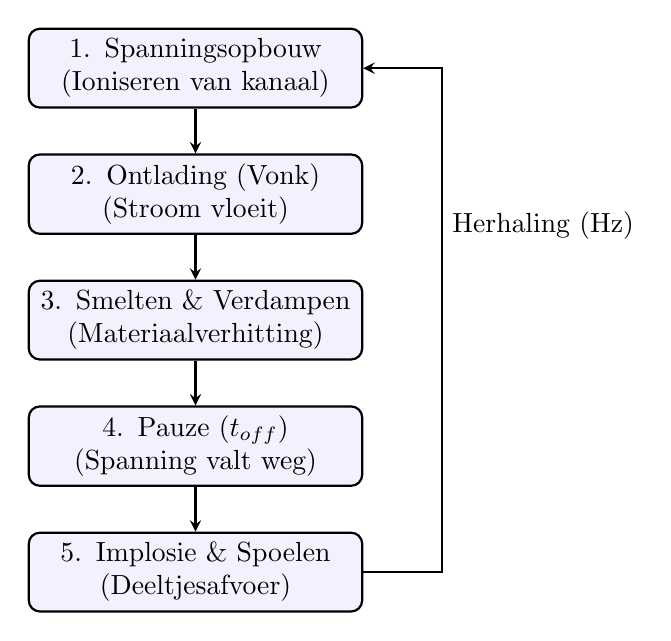
\begin{tikzpicture}[node distance=1.6cm, auto,
            procstep/.style={rectangle, draw=black, thick, fill=blue!5, text width=4cm, align=center, rounded corners, minimum height=1cm},
            arrow/.style={thick, ->, >=stealth}
        ]
        \node (start) [procstep] {1. Spanningsopbouw \\ (Ioniseren van kanaal)};
        \node (spark) [procstep, below of=start] {2. Ontlading (Vonk) \\ (Stroom vloeit)};
        \node (heat)  [procstep, below of=spark] {3. Smelten \& Verdampen \\ (Materiaalverhitting)};
        \node (off)   [procstep, below of=heat] {4. Pauze ($t_{off}$) \\ (Spanning valt weg)};
        \node (flush) [procstep, below of=off] {5. Implosie \& Spoelen \\ (Deeltjesafvoer)};

        \draw [arrow] (start) -- (spark);
        \draw [arrow] (spark) -- (heat);
        \draw [arrow] (heat) -- (off);
        \draw [arrow] (off) -- (flush);
        \draw [arrow] (flush.east) -- ++(1,0) |- node[anchor=west, yshift=-2cm] {Herhaling (Hz)} (start.east);

    \end{tikzpicture}
    \caption{Cyclus van één EDM-puls: van spanningsopbouw tot spoelen.}
    \label{fig:edm_puls_flow}
\end{figure}

Je benedenplaat wordt \textbf{negatief geladen} en de elektrode \textbf{positief}.
Er is dan een puls van \textbf{discharge} die een stukje materiaal wegneemt.
\textbf{Pulsen} hebben een \textbf{frequentie} tussen ongeveer \SI{100}{kHz} en \SI{1}{MHz}.
Je genereert dan veel discharges die opbouwen zodat je lijnen stap per stap kunt wegnemen.
\newline
De afstand tussen de elektrode en het werkstuk is enorm klein maar enorm belangrijk.
Raakt de elektrode het werkstuk, dan krijg je \textbf{kortsluiting} en stopt het vonken.
\newline
De weggenomen deeltjes zijn \textbf{bolvormig}: het gesmolten metaal wordt de vloeistof in geslingerd
en stolt daar tot kleine bolletjes.
\newline
De pulsenergie wordt gegeven door de formule
\frm{Pulsenergie tijdens vonkfrezen}{W_e = \int_0^{t_e} U_e I_e \, dt}{waarbij $W_e$ de pulsenergie is [\si{J}], $U_e$ de doorslagspanning [\si{V}], $I_e$ de stroom [\si{A}] en $t_e$ de pulstijd [\si{s}].}
\begin{figure}[htbp]
    \centering
    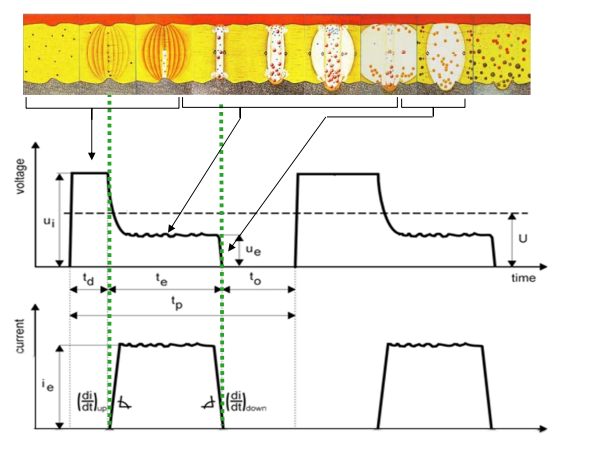
\includegraphics[width=0.3\textwidth]{assets/image61.png}
    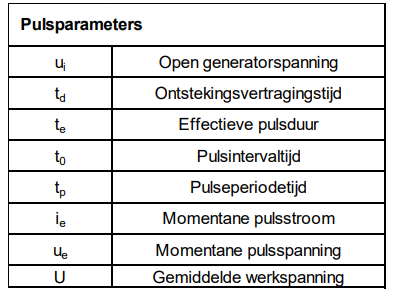
\includegraphics[width=0.3\textwidth]{assets/image62.png}
    \caption{Stapsgewijs een puls en de bijbehorende spannings- en stroomcurves en tabel van alle parameters.}
    \label{fig:edm_elektrode_vormen.png}
\end{figure}
\FloatBarrier

Het vonkproces verloopt in drie cyclische fases die zich duizenden keren per seconde herhalen:

\begin{figure}[ht]
    \centering
    \begin{tikzpicture}[scale=0.9,
            elec/.style={fill=gray!30, draw=black, thick},
            work/.style={fill=gray!10, draw=black, thick, pattern=north east lines},
            gas/.style={circle, draw=blue!50, fill=blue!10, dashed, minimum size=1.5cm},
            spark/.style={decoration={zigzag, segment length=1mm, amplitude=0.5mm}, decorate, draw=orange, very thick}
        ]
        % Phase 1: Initiation
        \begin{scope}[local bounding box=p1]
            \node at (0, 3) {\textbf{1. Initiatie}};
            \draw[elec] (-1, 2.5) -- (-1, 1.5) -- (0, 0.5) -- (1, 1.5) -- (1, 2.5) -- cycle;
            \draw[work] (-1.5, -1) rectangle (1.5, 0);

            % Ions
            \foreach \x in {-0.5, -0.2, 0.2, 0.5} \node[circle, fill=red, inner sep=1pt] at (\x, 0.2) {\tiny $+$};
            \foreach \x in {-0.6, 0, 0.6} \node[circle, fill=blue, inner sep=1pt] at (\x, -0.2) {\tiny $-$};
            \node[font=\footnotesize, align=center] at (0, -1.5) {Veldopbouw \& \\ Ionisatie};
        \end{scope}

        % Phase 2: Discharge
        \begin{scope}[xshift=4.5cm, local bounding box=p2]
            \node at (0, 3) {\textbf{2. Discharge}};
            \draw[elec] (-1, 2.5) -- (-1, 1.5) -- (0, 0.5) -- (1, 1.5) -- (1, 2.5) -- cycle;
            \draw[work] (-1.5, -1) rectangle (1.5, 0);

            % Gas bubble & Spark
            \node[gas] at (0, 0.25) {};
            \draw[spark] (0, 0.5) -- (0, 0);

            \node[font=\footnotesize, align=center] at (0, -1.5) {Plasmakanaal \& \\ Smelten};
        \end{scope}

        % Phase 3: Ejection
        \begin{scope}[xshift=9cm, local bounding box=p3]
            \node at (0, 3) {\textbf{3. Uitstoot}};
            \draw[elec] (-1, 2.5) -- (-1, 1.5) -- (0, 0.5) -- (1, 1.5) -- (1, 2.5) -- cycle;
            % Crater
            \draw[work] (-1.5, 0) -- (-0.3, 0) arc(180:360:0.3) -- (1.5, 0) -- (1.5, -1) -- (-1.5, -1) -- cycle;

            % Debris
            \foreach \r in {0.1, 0.3, 0.5} \fill[black] (\r, 0.5) circle (1pt);
            \foreach \r in {-0.2, 0.2} \fill[black] (\r, 0.8) circle (1pt);

            \node[font=\footnotesize, align=center] at (0, -1.5) {Implosie \& \\ Materiaalafname};
        \end{scope}
    \end{tikzpicture}
    \caption{De drie fases van een EDM-puls.}
    \label{fig:edm_phases}
\end{figure}

\begin{enumerate}
    \item \textbf{De initiatiefase (Ontsteking):}
          Er wordt een spanning aangelegd tussen elektrode en werkstuk. Het elektrisch veld zorgt ervoor dat
          vrije elektronen en ionen in het diëlektricum versnellen en botsen.
          Dit creëert een \emph{sneeuwbaleffect} (lawine-ionisatie), waardoor er een geleidend ionisatiekanaal ontstaat.

    \item \textbf{De dischargefase (Ontlading):}
          Zodra het kanaal geleidend is, volgt de hoofdontlading (de vonk).
          De stroomsterkte piekt en er ontstaat een \textbf{gasbel} van plasma rondom de vonk.
          De ionen botsen met hoge kinetische energie op het werkstuk, wat wordt omgezet in extreme hitte ($8000\text{--}12000\,^\circ\text{C}$).
          Hierdoor smelt en verdampt een klein deel van het werkstuk (en in mindere mate de elektrode).

    \item \textbf{De uitstootfase (Implosie):}
          De stroom wordt plotseling onderbroken (shutdown).
          De temperatuur daalt en de gasbel implodeert krachtig.
          Door deze implosie wordt het gesmolten materiaal uit de krater weggeschoten in het diëlektricum,
          waar het stolt tot kleine bolletjes (swarf). Het diëlektricum spoelt de opening schoon voor de volgende puls.
\end{enumerate}

\begin{figure}[ht]
    \centering
    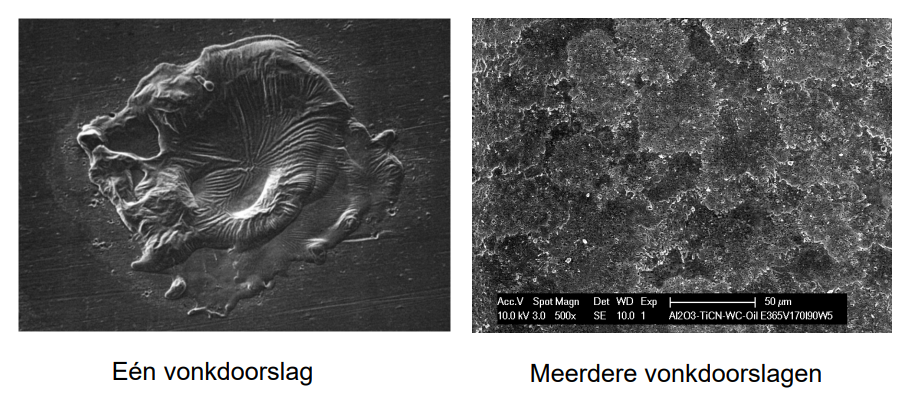
\includegraphics[width=0.6\textwidth]{assets/image63.png}
    \caption{Een vonk in vergelijking met meerdere vonken}
    \label{fig:1vonkenmeerderevonken.png}
\end{figure}

\section{Performance van EDM}

De materiaalafname (material removal rate, MRR) wordt uitgedrukt in kubieke centimeter per minuut.
Ze ligt veel lager dan bij verspanen; dat is meteen het grootste nadeel van EDM.
\newline
Ook gereedschapsslijtage is een probleem bij EDM. We drukken die uit als een verhouding:
\frm{Gereedschapsslijtage bij EDM}{\vartheta = \frac{V_{\text{elektrode}}}{V_{\text{werkstuk}}}}{waarbij $\vartheta$ de relatieve slijtage is [-], $V_{\text{elektrode}}$ het versleten volume van de elektrode [\si{mm^3}] en $V_{\text{werkstuk}}$ het weggenomen volume van het werkstuk [\si{mm^3}]. Typisch tussen $1\%$ en $5\%$.}
De oppervlaktekwaliteit $R_a$ is afhankelijk van je settings. Je kunt afhankelijk van de stroom die je gebruikt andere oppervlaktekwaliteit krijgen.
\newline
\textbf{Hoge energie -> hoge materiaalafname maar slechte oppervlaktekwaliteit.}
\textbf{Lage energie -> lage materiaalafname maar goede oppervlaktekwaliteit.}
\newline
Je krijgt ook een harde \textbf{thermisch aangetaste zone (TAZ)} aan het oppervlak:
een laag die door de hitte van de vonk van structuur veranderd is.

\begin{figure}[ht]
    \centering
    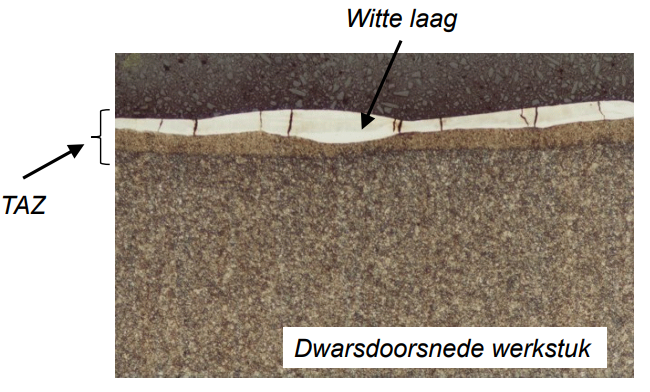
\includegraphics[width=0.5\textwidth]{assets/image64.png}
    \caption{TAZ, thermisch aangetaste zone bij EDM}
    \label{fig:taz_edm.png}
\end{figure}
\FloatBarrier

$\rightarrow$ Deze zone smelt op en stolt daarna razendsnel terug. Daardoor ontstaan er microscheuren in het oppervlak.
Dat is slecht voor de vermoeiingssterkte; de laag moet weggewerkt worden door te slijpen of te frezen (zie hybrideprocessen).

\section{Spleetregeling}
De grootte van de spleet hangt af van de ontsteekvertraging $t_d$: de tijd tussen het aanleggen van de
spanning en het doorslaan van de vonk. Hoe groter de spleet, hoe langer $t_d$.
Is $t_d$ te lang, dan staat de elektrode te ver en komt er geen vonk meer.
Is de spleet te klein, dan krijg je kortsluiting.
Je moet dus een goede regeling hebben die de afstand tussen elektrode en werkstuk regelt.
\newline
Door $t_d$ te meten kun je de afstand regelen.
\newline
Vroeger werd dat handmatig gedaan maar nu gebeurt dat automatisch met computers.
\subsection{Elektrodemateriaal}
\begin{figure}[ht]
    \centering
    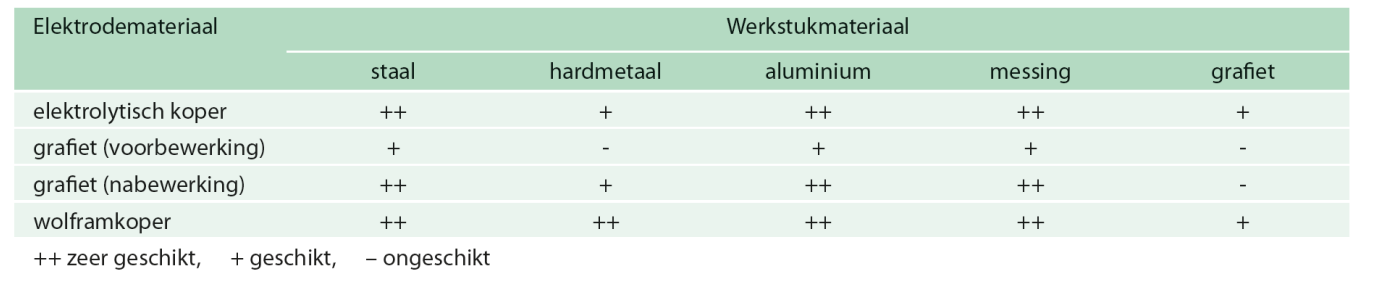
\includegraphics[width=0.8\textwidth]{assets/image65.png}
    \caption{Elektrode materialen voor EDM}
    \label{fig:image65.png}
\end{figure}

Je wilt een materiaal dat erosievast is, zodat je elektrode minder snel slijt. Dat drukken we uit met:
\frm{Erosievastheid van elektrode (schematische benadering)}
{E = \lambda \cdot \rho \cdot c \cdot T_m}
{waarbij $E$ de erosievastheid is [\si{J^2 \cdot s^{-1} \cdot m^{-4} \cdot K}], \(\lambda\) de warmtegeleidingscoëfficiënt [\si{W/(m.K)}], \(\rho\) de massadichtheid [\si{kg/m^3}], \(c\) de soortelijke warmte [\si{J/(kg.K)}] en \(T_m\) de smelttemperatuur [\si{K}].}

\vspace{0.5cm}
\section{Effecten van pulsduur en stroomsterkte}

\vspace{0.5cm}


\begin{figure}[ht]
    \centering
    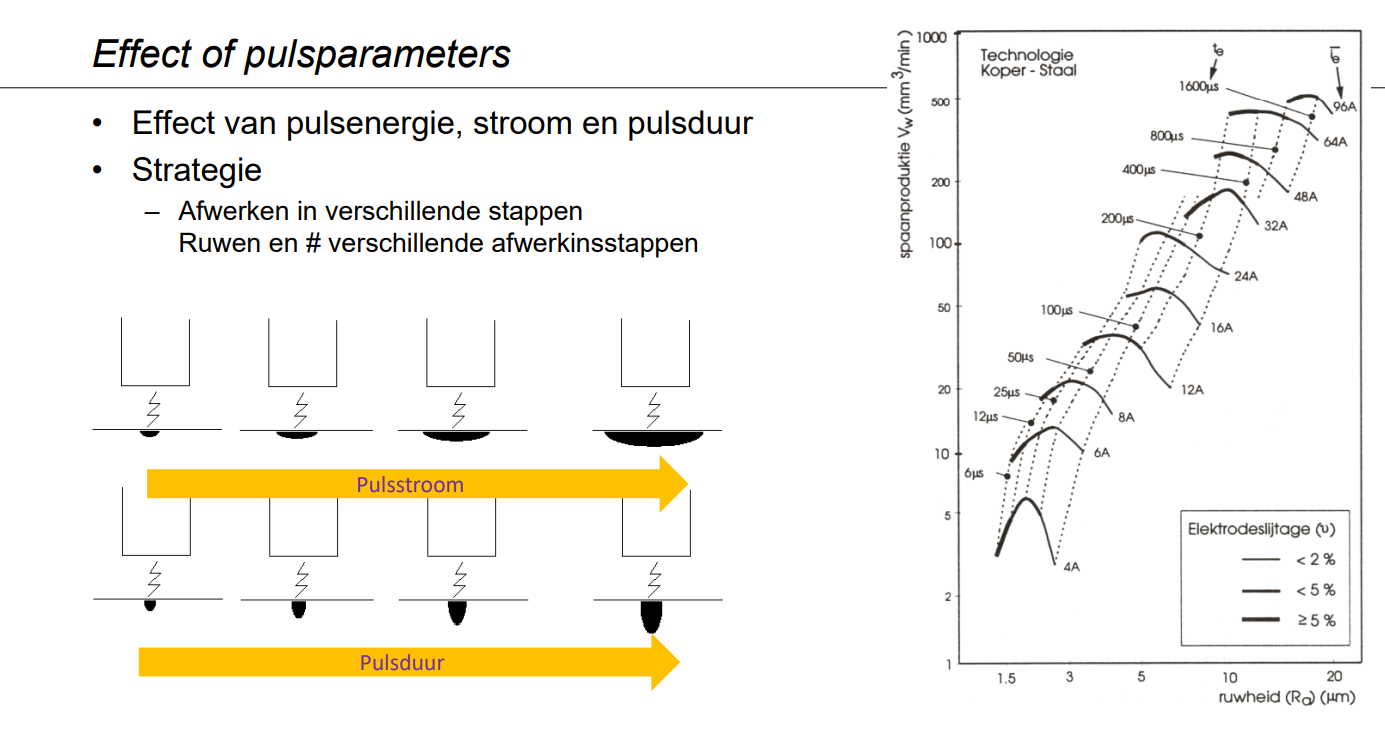
\includegraphics[width=0.8\textwidth]{assets/image66.png}
    \caption{Effecten van pulsduur en stroomsterkte bij EDM}
    \label{fig:Effecten_pulsduur_stroomsterkte.png}
\end{figure}
\FloatBarrier

Dikkere lijnen betekenen grotere elektrodeslijtage. Bij kortere pulsen heb je meer slijtage.
Dat komt omdat elektronen veel lichter zijn dan ionen: bij het begin van de puls zijn zij als eerste op snelheid
en bombarderen ze de \emph{anode}. Pas bij langere pulsen krijgen de zware, trage ionen de tijd om de kathode
te bereiken. Korte pulsen belasten dus vooral de positieve elektrode.

\section{Toepassingen}
\begin{itemize}
    \item Vonkerosie laat bewerken van harde materialen toe.
    \item Je kunt complexe vormen maken die met andere processen moeilijk te maken zijn. Je kunt profielen maken
          met hoge nauwkeurigheid die dan caviteiten maken.
    \item Slanke gereedschappen en dunne wanden zijn mogelijk omdat er geen mechanische krachten optreden tijdens het bewerken.
\end{itemize}

\subsection{Types}

\begin{figure}[htbp]
    \centering
    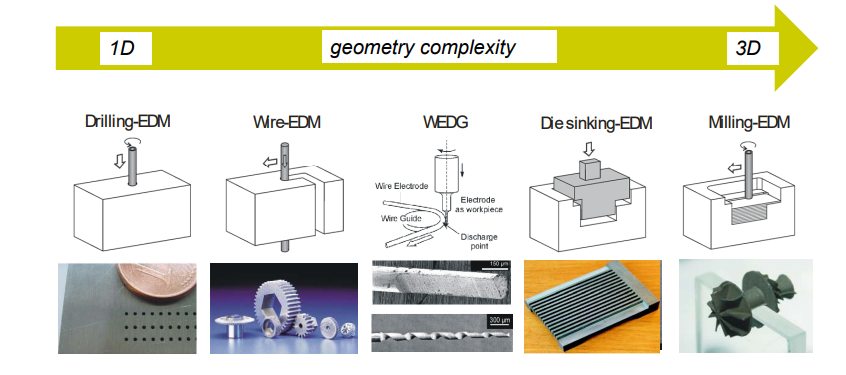
\includegraphics[width=0.8\textwidth]{assets/image67.png}
    \caption{Verschillende types vonkerosie}
    \label{fig:verschillende_types_vonkerosie.png}
\end{figure}
\FloatBarrier
\subsection{Zinkvonkerosie}

\begin{figure}[htbp]
    \centering
    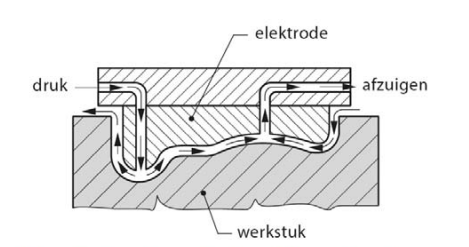
\includegraphics[width=0.3\textwidth]{assets/image68.png}
    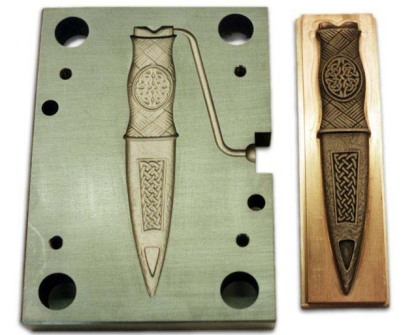
\includegraphics[width=0.3\textwidth]{assets/image69.png}
    \caption{Zinkvonkenrosie proces}
    \label{fig:Zinkvonkenrosie.png}
\end{figure}
\FloatBarrier

Bij zinkvonken laat je een geleidend profiel (de elektrode) langzaam in het werkstuk zakken.
Je moet de erosiedeeltjes voortdurend uit het diëlektricum spoelen, anders begint dat te geleiden
en krijg je ongecontroleerde ontladingen.
Je maakt zo het \emph{inverse} profiel van de elektrode in het werkstuk.

Je kunt er ook enorm kleine details mee maken, tot rond \SI{6}{\micro m}, zolang je de elektrode
zelf op die maat kunt maken.


\subsection{Draadvonkerosie}
Voor een inwendige contour moet je eerst een startgat maken in het werkstuk, met zinkvonken of met boren.
Daar steek je de draad door, en dan zaag je met die draad je contour.

Draadvonken verdraagt geen lange pulsen: de draad is zo dun dat hij anders zelf zou smelten.
Je werkt dus met heel korte pulsen, hoog in het frequentiebereik.
Maar kortere pulsen eroderen de elektrode juist sneller (zie de figuur hierboven).
De oplossing is de polariteit om te draaien, zodat het elektronenbombardement op het \emph{werkstuk}
terechtkomt en niet op de draad. Zo beschadig je de draad minder.

\subsection{WEDG}
\textbf{Wire Electro Discharge Grinding}
is een proces waarbij een draad als elektrode wordt gebruikt om zeer nauwkeurige en fijne bewerkingen
uit te voeren op harde materialen.

\subsection{Die sinking EDM}
Je hebt een elektrode die de vorm heeft van wat je wilt maken.
Je laat die elektrode naar beneden zakken en zo maak je een caviteit in het werkstuk.
\subsection{Milling EDM}
Je hebt een ronde elektrode die ronddraait en zo materiaal weghaalt.
\subsection{Planetair vonken}
Je laat de elektrode een kleine cirkelbeweging maken, zodat je een caviteit krijgt die \emph{groter}
is dan de elektrode zelf. Handig om met één elektrode zowel te ruwen als te finishen.
\subsection{Contourvonken}
Via NC-sturing kun je heel kleine dingen maken, zoals matrijzen voor kleine tandwielen.
Enorm veel microbewerkingen kunnen zo gemaakt worden.

\belangrijk{Belangrijk}
Vonkerosie zet geen enkele mechanische kracht op het werkstuk.
De materialen moeten wel elektrisch geleidend zijn: een soortelijke weerstand lager dan ongeveer $100\,\Omega\,$cm.

\begin{figure}[htbp]
    \centering
    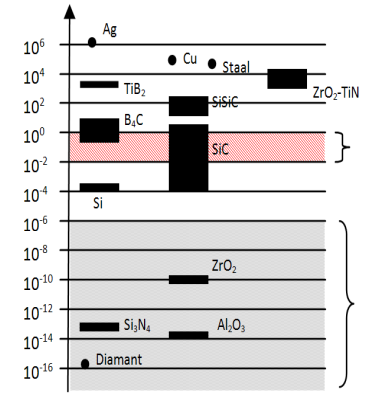
\includegraphics[width=0.3\textwidth]{assets/image70.png}
    \caption{}
    \label{fig:image70.png}
\end{figure}
\FloatBarrier

\subsection{Vonken van keramieken}

\begin{figure}[htbp]
    \centering
    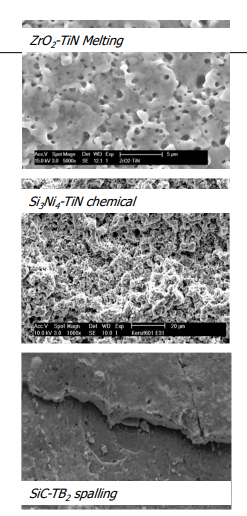
\includegraphics[width=0.2\textwidth]{assets/image71.png}
    \caption{Ruw oppervlak met scheuren door spalling bij keramieken}
    \label{fig:vonken_keramieken.png}
\end{figure}
\FloatBarrier


Keramieken zijn van nature isolerend en
kunnen daarom normaal niet met EDM worden bewerkt.
Om ze toch bewerkbaar te maken,
worden ze geleidend gemaakt door toevoeging van geleidende deeltjes
(zoals siliciumcarbide of titaannitride).
Tijdens het \textbf{sinteren} wordt dit mengsel van poeders
onder hoge temperatuur en druk samengeperst tot een solide massa.
Door dit proces ontstaat een intern netwerk van geleidende paden,
waardoor de elektrische weerstand voldoende daalt (typisch < $100\,\Omega\text{cm}$) om het vonkproces mogelijk te maken.

Wat er kan gebeuren als je hierop gaat vonken, is dat er scheuren ontstaan in het oppervlak van het keramiek.
Keramiek is bros, dus de thermische schok van de vonk doet het barsten.
Wordt er dan nóg eens op dezelfde plek gevonkt, dan breken er stukjes af. Dat noemen we \textbf{spalling}
(afschilferen).

In de industrie stelde men vast dat juist de \emph{fijne} instellingen, bedoeld om keramiek nauwkeuriger
af te werken, het meeste spalling gaven: hoe meer men het oppervlak probeerde te verbeteren,
hoe slechter het werd.

\section{Elektrochemische bewerkingen}

\begin{conceptbox}[ECM (Electro Chemical Machining)]
    ECM is gebaseerd op gecontroleerde elektrolyse (anodische oplossing).
    In tegenstelling tot EDM is ECM een \keyterm{chemisch} proces zonder warmteontwikkeling of gereedschapsslijtage. Het werkstuk fungeert als anode en lost op in een geleidend elektrolyt.
\end{conceptbox}

Je neemt een werkstuk en een elektrode en dompelt beide in een elektrolytische vloeistof.
Je brengt de elektrode heel dicht bij het werkstuk (zonder contact) en laat er een stroom door lopen.
De stroomdichtheden liggen in de orde van \SI{50}{A/cm^2} tot \SI{1000}{A/cm^2}.
Het werkstuk is de anode en de elektrode is de kathode.
Je beweegt het werkstuk stap voor stap naar beneden om materiaal chemisch te verwijderen.
\newline
$\rightarrow$ Je krijgt een \textbf{elektrolysereactie} tussen de twee.
\newline
\begin{figure}[ht]
    \centering
    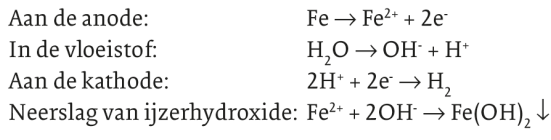
\includegraphics[width=0.45\textwidth]{assets/image72.png}
    \caption{Principe van elektrochemisch bewerken: het werkstuk (anode) lost op in de elektrolyt.}
    \label{fig:ecm_principe}
\end{figure}
De anode (het werkstuk) lost op in de elektrolyt door oxidatie.
De kathode (de elektrode) blijft intact door reductie.
\newline
Voorbeeld bij anode van ijzer in een zoutoplossing \ce{NaCl}, \ce{H2O} als elektrolyt:
\begin{itemize}
    \item \textbf{Anode (Werkstuk) - Oxidatie:}
          \[ \ce{Fe -> Fe^{2+} + 2 e-} \]
          Het ijzer gaat in oplossing als positieve ionen.
    \item \textbf{Kathode (Gereedschap) - Reductie:}
          \[ \ce{2 H2O + 2 e- -> H2 ^ + 2 OH-} \]
          Waterstofgas ontsnapt en hydroxylionen worden gevormd.
    \item \textbf{Totaalreactie in elektrolyt:}
          \[ \ce{Fe^{2+} + 2 OH- -> Fe(OH)2 v} \]
          Je krijgt een neerslag van ijzerhydroxide, deze moet worden weggepompt.
\end{itemize}

Het verschil met vonkerosie is dat je bij vonkerosie een
isolerend diëlektricum hebt en bij elektrochemisch bewerken
een geleidend elektrolyt. Je hebt dus geen
slijtage van de elektrode bij elektrochemisch bewerken.
\newline

\subsection{Eigenschappen van elektrochemisch bewerken}
\begin{itemize}
    \item Heel goede oppervlaktekwaliteit (laag $R_a$)
    \item Geen gereedschapslijtage
    \item Geen thermisch beïnvloede zone (geen TAZ): het oppervlak is niet aangetast
    \item Niet super nauwkeurig: de caviteit wordt breder dan de elektrode zelf (typisch $\pm$ 0,1 tot 1,0 mm ``overcut'')
    \item Niet goed voor het milieu: je houdt een elektrolyt vol metaalhydroxideslib over
\end{itemize}

Het nadeel is dus dat je meer materiaal wegneemt dan strikt de vorm van je elektrode.
\begin{figure}[ht]
    \centering
    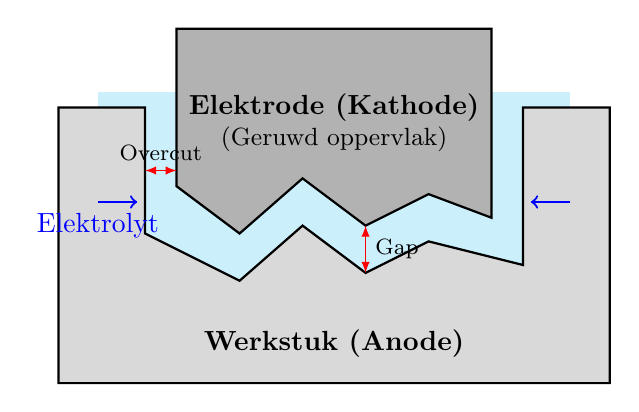
\begin{tikzpicture}
        % Styles
        \tikzset{
            tool/.style={fill=gray!60, draw=black, thick},
            workpiece/.style={fill=gray!30, draw=black, thick},
            electrolyte/.style={fill=cyan!20},
            dim/.style={draw=red, <->, >=latex, font=\footnotesize}
        }

        % Tool Coordinates (Rough bottom)
        \coordinate (T1) at (-2.0, 1.0);
        \coordinate (T2) at (-1.2, 0.4);
        \coordinate (T3) at (-0.4, 1.1);
        \coordinate (T4) at (0.4, 0.5);
        \coordinate (T5) at (1.2, 0.9);
        \coordinate (T6) at (2.0, 0.6);

        % Draw Electrolyte (Background in gap)
        \fill[electrolyte] (-3, -1) rectangle (3, 2.2);

        % Draw Tool
        \draw[tool] (-2, 3) -- (2, 3) -- (2.0, 0.6) -- (1.2, 0.9) -- (0.4, 0.5) -- (-0.4, 1.1) -- (-1.2, 0.4) -- (-2.0, 1.0) -- cycle;
        \node at (0, 2) {\textbf{Elektrode (Kathode)}};
        \node at (0, 1.6) {\small (Geruwd oppervlak)};

        % Draw Workpiece
        \draw[workpiece] (-3.5, 2.0) -- (-2.4, 2.0) -- (-2.4, 0.4) -- (-1.2, -0.2) -- (-0.4, 0.5) -- (0.4, -0.1) -- (1.2, 0.3) -- (2.4, 0.0) -- (2.4, 2.0) -- (3.5, 2.0) -- (3.5, -1.5) -- (-3.5, -1.5) -- cycle;
        \node at (0, -1) {\textbf{Werkstuk (Anode)}};

        % Dimensions / Annotations
        % Side Overcut
        \draw[dim] (-2.4, 1.2) -- (-2.0, 1.2) node[midway, above] {Overcut};
        % Bottom Gap
        \draw[dim] (0.4, -0.1) -- (0.4, 0.5) node[midway, right] {Gap};

        % Electrolyte flow
        \draw[->, blue, thick] (-3, 0.8) -- (-2.5, 0.8);
        \draw[->, blue, thick] (3, 0.8) -- (2.5, 0.8);
        \node[blue] at (-3, 0.5) {Elektrolyt};

    \end{tikzpicture}
    \caption{Schematische weergave van elektrochemisch bewerken (ECM) met een ruwe elektrode. De ontstane caviteit in het werkstuk is groter dan de elektrode door de "overcut" en de chemische werking.}
    \label{fig:ecm_overcut}
\end{figure}

Precies dat maakt ECM handig \emph{na} zinkvonken: vonkeroderen laat een geharde, gescheurde laag achter
door het snel opwarmen en afkoelen van het materiaal.
ECM neemt die laag weg en geeft een goede oppervlaktekwaliteit.
Typische overcut-waarden bij ECM liggen tussen ongeveer 0,13 en 1,0 mm,
bij micro-ECM zijn waardes rond 0,02 mm mogelijk.
\newline

\subsection{Afname bij ECM}
\frm{Afnamesnelheid bij ECM (MRR, material removal rate)}{MRR = \dfrac{I \cdot A}{F \cdot V}\cdot \eta}{waarbij $MRR$
de afnamesnelheid is [\si{g/s}],
$I$ de stroomsterkte [\si{A}], $A$ de atoommassa [\si{g/mol}], $V$ de valentie [-], $F$ de Faraday-constante
(\(96485\,\mathrm{C/mol}\)) en $\eta$ de efficiëntie [-].}
\begin{voorbeeld}[ECM — titaan]
    Voorbeeld bij titaan: \(A=48\ \si{g/mol}\), \(V=3\), \(I=2000\ \si{A}\) en \(\eta=0{,}9\).
    \[
        M_{\mathrm{ECM}}=\frac{I\cdot A}{F\cdot V}\cdot\eta
        =\frac{2000\cdot48}{96485\cdot3}\cdot0{,}9\approx0{,}298\ \si{g/s}.
    \]
    Omrekenen naar \(\si{cm^3/min}\) met \(\rho_{\mathrm{Ti}}=4.51\ \si{g/cm^3}\):
    \[
        \dot V=\frac{0{,}298\ \si{g/s}}{4{,}51\ \si{g/cm^3}}\cdot60\ \si{s/min}\approx3{,}97\ \si{cm^3/min}.
    \]
\end{voorbeeld}


\subsection{Toepassingen van ECM}
Je kunt ECM gebruiken voor:
\begin{itemize}
    \item Het bewerken van harde materialen zoals titanium en superlegeringen.
    \item Het maken van complexe vormen en fijne details die moeilijk te bereiken zijn met conventionele methoden.
    \item Het produceren van onderdelen met hoge oppervlaktekwaliteit zonder thermische of mechanische schade.
    \item Is gebruikt voor het maken van turbinebladen, raketonderdelen, medische implantaten, en micro-elektronische componenten.
\end{itemize}


\textbf{Afname zonder Stroom}
Je zet een masker op het werkstuk zodat alleen de delen die je wilt bewerken blootliggen.
De \textbf{etsvloeistof} vreet dan alleen de onbedekte delen weg; hier is dus geen stroom nodig.
Omdat de etsvloeistof in alle richtingen even hard werkt, vreet ze ook zijdelings onder het masker.
Dat noemen we \textbf{ondersnijding}.
\begin{figure}[htbp]
    \centering
    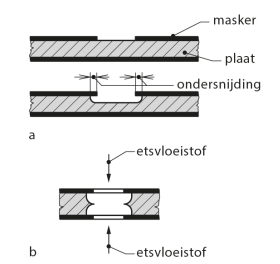
\includegraphics[width=0.4\textwidth]{assets/image75.png}
    \caption{Wegeroderen van materiaal zonder stroom met etsvloeistof}
    \label{fig:eroderen_etsvloeistof.png}
\end{figure}

De etstijd bepaalt hoeveel materiaal je wegneemt en dus ook hoe groot de ondersnijding wordt.



\textbf{Fotoetsen} is een gelijkaardig proces, maar dan voor heel kleine details.
Je maskeert het oppervlak met een lichtgevoelige laklaag (fotoresist).
Daarover leg je een masker met transparante en niet-transparante zones.
UV-licht valt door de transparante zones en verandert daar de lak, zodat die weggespoeld kan worden.
De blootgelegde patronen ets je dan weg met etsvloeistof.
Die patronen kunnen enorm klein zijn, tot rond de micrometer; dit is de basis van de micro-elektronica.

Net zoals bij normaal etsen krijg je ook ondersnijding waar je rekening mee moet houden.

\begin{figure}[htbp]
    \centering
    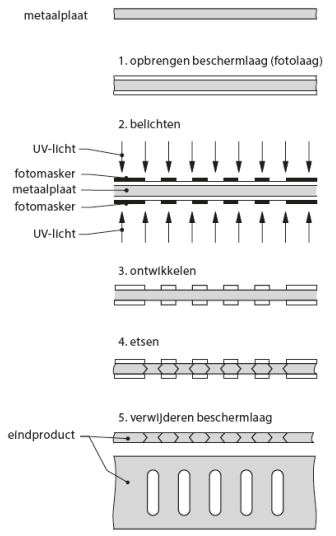
\includegraphics[width=0.26\textwidth]{assets/image73.png}
    \caption{Fotoetsen van een complex onderdeel met ECM}
    \label{fig:foto_etsen_ecm.png}
\end{figure}

\section{Ultrasoon bewerken (Ultrasonic Machining)}
\FloatBarrier

\begin{wrapfigure}[17]{r}{0.4\textwidth}
    \centering
    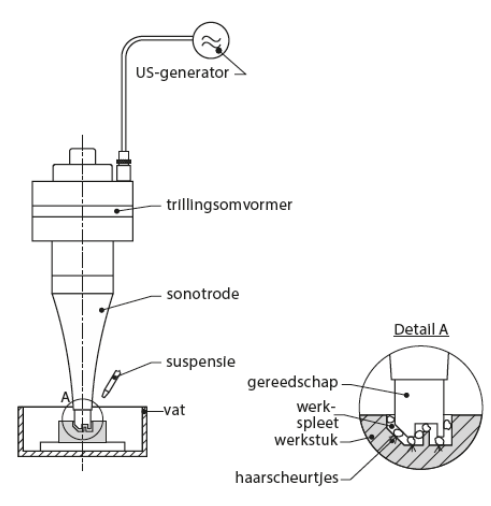
\includegraphics[width=\linewidth]{assets/image74.png}
    \caption{Principe van ultrasoon bewerken}
    \label{fig:principe_ultrasoon_bewerken.png}
\end{wrapfigure}


Ultrasoon bewerken is een bewerkingsproces waarbij hoogfrequente trillingen gebruikt worden om materiaal van een werkstuk te verwijderen.
Het proces maakt gebruik van een sonotrode die ultrasone trillingen (typisch tussen \SI{20}{kHz} en \SI{40}{kHz})
met een heel kleine amplitude genereert.
Die trillingen slaan, via een suspensie van abrasieve korrels, microscheurtjes in het oppervlak,
waarna er kleine deeltjes uitbreken.
De techniek werkt goed voor harde en \emph{brosse} materialen zoals keramiek, glas en gehard staal,
juist omdat die slecht tegen scheurtjes kunnen. Je hamert als het ware op het materiaal.

Ductiele materialen zoals metalen zijn ook bewerkbaar:
Door de enorm grote trillingen krijg je een \textbf{vermoeiingsproces} in het materiaal waardoor je ook materiaal kunt wegnemen.

\begin{figure}[htbp]
    \centering
    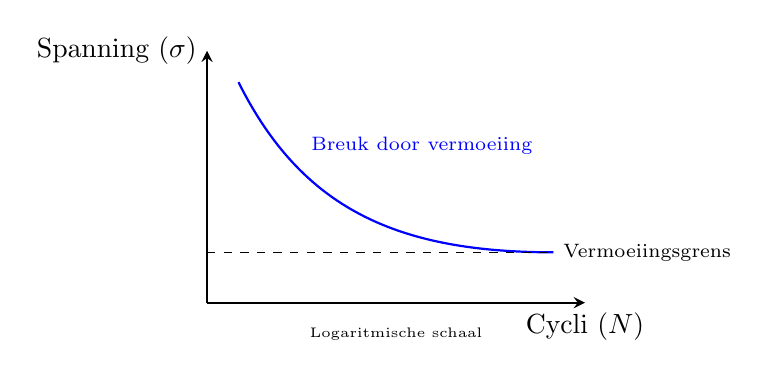
\begin{tikzpicture}[scale=0.8]
        % Axes
        \draw[thick,->,>=stealth] (0,0) -- (6,0) node[below] {Cycli ($N$)};
        \draw[thick,->,>=stealth] (0,0) -- (0,4) node[left] {Spanning ($\sigma$)};

        % Curve
        \draw[blue, thick] (0.5,3.5) .. controls (1.5,1.5) and (3,0.8) .. (5.5,0.8);

        % Annotations
        \node[blue, font=\scriptsize, anchor=west] at (1.5,2.5) {Breuk door vermoeiing};
        \draw[dashed] (0,0.8) -- (5.5,0.8) node[right, font=\scriptsize] {Vermoeiingsgrens};

        % Labels
        \node[font=\tiny] at (3,-0.5) {Logaritmische schaal};
    \end{tikzpicture}
    \caption{S-N curve (Wöhler-curve) die het vermoeiingsproces bij metalen weergeeft.}
    \label{fig:vermoeiing_sn}
\end{figure}
\FloatBarrier

Het gereedschap is gemaakt van taaie materialen zodat het niet snel slijt.
Het wordt vooral toegepast op harde materialen die moeilijk te bewerken zijn met conventionele methoden.
Je kunt ook een profiel maken van het gereedschap en dan dat profiel in het werkstuk maken.

\section{Straalbewerkingen}
Straalbewerkingen zijn processen waarbij een geconcentreerde straal van energie of materiaal wordt gebruikt om materiaal van een werkstuk te verwijderen of te bewerken.


\begin{engtable}[
        caption = {Overzicht van verschillende straalbewerkingen.},
        label = {tab:straalbewerkingen},
    ]{
        colspec = {l X X},
        width = \textwidth,
        cells = {font=\small},
        row{1} = {font=\bfseries},
    }
    Energiedrager & Bewerkingen & Toepassingen \\
    {Vloeistof (Water)} & Waterstraalsnijden (WJM) & Snijden van zachte materialen (plastic, textiel, voedsel). \\
    {Vloeistof + Abrasief} & Abrasief waterstraalsnijden (AWJM) & Snijden van harde materialen (metaal, glas, steen). \\
    {Licht (Fotonen)} & Laserstraalbewerking (LBM) & Snijden, lassen en boren van bijna alle materialen. \\
    Elektronen & Elektronenstraalbewerking (EBM) & Zeer nauwkeurig boren en snijden (in vacuüm). \\
    Ionen & Ionenstraalbewerking (IBM) & Etsen op nanoschaal en oppervlaktebewerking. \\
    Gas / Plasma & Plasmastralen (PAM) & Ruw snijden van dikke metaalplaten. \\
\end{engtable}

\subsection{Shotpeening}
Korrels worden met hoge snelheid op het oppervlak van een werkstuk geschoten.
Dit veroorzaakt plastische vervorming aan het oppervlak, wat leidt tot een verhoogde vermoeiingssterkte
door de inwendige spanningen die worden geïnduceerd.
\subsection{Abrasief stralen}
Je gebruikt een straal van abrasieve deeltjes (zoals zand)
die met hoge snelheid op het oppervlak van een werkstuk worden gespoten.
Dit wordt vaak gebruikt voor het \textbf{reinigen, ontroesten of matten} van oppervlakken.
Het proces werkt volgens de wet van Bernoulli (zie Warmte en stromingen).

\textbf{Wet van Bernoulli}
In een stromend fluïdum is de som van de drukenergie, kinetische energie en potentiële energie per eenheid volume constant langs een stroomlijn:
\[
    P + \frac{1}{2} \rho v^2 + \rho gh = \text{constant}
\]
waarbij \(P\) de druk is, \(\rho\) de dichtheid van het fluïdum, \(v\) de stroomsnelheid, \(g\) de zwaartekrachtversnelling en \(h\) de hoogte boven een referentieniveau.


De deeltjes moeten hun kinetische energie kwijt op het oppervlak; die energie gaat in het losslaan
van kleine deeltjes materiaal.
\subsection{Waterstraalsnijden}
Water wordt bij \textbf{4000 bar} door een heel kleine opening gepompt.
De straal die daaruit komt heeft zoveel kinetische energie dat hij materiaal wegsnijdt.
Je kunt er dikke stukken mee doorsnijden.
\newline
Er komt geen warmte aan te pas, dus je hebt geen thermisch aangetaste zone (TAZ).
Daardoor is het ook bruikbaar in andere sectoren, zoals de voedingsindustrie.

\begin{figure}[ht]
    \centering
    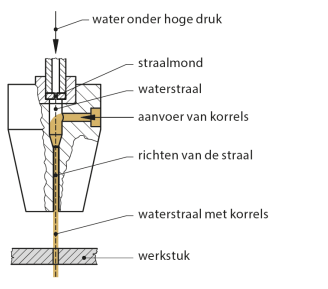
\includegraphics[width=0.4\textwidth]{assets/image76.png}
    \caption{Waterstraal snijden proces}
    \label{fig:image76.png}
\end{figure}

Een extra mogelijkheid is het gebruik van ijsbolletjes om oppervlakken te reinigen in plaats van zand.
Het ijs smelt gewoon weg, dus je moet achteraf geen zand opruimen.

\section{Laserstraalbewerking (LBM)}
\subsection{Hoe werkt een laser?}
Een laser is een geconcentreerde lichtbron die op één specifieke golflengte licht uitzendt,
met hoge intensiteit en coherentie.

\begin{conceptbox}[LASER]
    \textbf{L}ight \textbf{A}mplification by \textbf{S}timulated \textbf{E}mission of \textbf{R}adiation:
    een apparaat dat licht versterkt door gestimuleerde emissie van straling.
\end{conceptbox}

Om een laser te maken breng je de atomen van het lasermedium naar een hogere energietoestand
door er energie in te pompen: het \concept{pompproces}.
Wanneer die atomen terugvallen naar hun lagere energietoestand, zenden ze fotonen uit.
Dat noemen we \concept{spontane emissie}.

Als zo'n foton een ander aangeslagen atoom treft, kan het dat atoom stimuleren om óók een foton uit te zenden,
identiek aan het eerste (zelfde frequentie, fase en richting).
Dat noemen we \concept{gestimuleerde emissie}. Doordat het licht heen en weer kaatst tussen twee spiegels,
wordt dit effect steeds versterkt.

Het resultaat is een coherente en monochromatische lichtstraal met hoge intensiteit.

\textbf{Workflow: Hoe een laser wordt gecreëerd}
\begin{figure}[ht]
    \centering
    \begin{tikzpicture}[
            node distance=0.6cm and 2cm,
            block/.style={rectangle, draw, fill=blue!10, text width=10cm, text centered, rounded corners, minimum height=0.8cm, thick, font=\small},
            line/.style={draw, thick, ->, >=stealth}
        ]
        % Nodes using relative positioning to avoid overlap
        \node (pumping) [block] {\textbf{1. Pompproces (Pumping)}: Toevoeren van energie om atomen naar hogere toestand te brengen.};

        \node (spontaneous) [block, below=of pumping] {\textbf{2. Spontane Emissie}: Atomen vallen terug en zenden ongeordende fotonen uit.};

        \node (stimulated) [block, below=of spontaneous] {\textbf{3. Gestimuleerde Emissie}: Fotonen treffen aangeslagen atomen $\to$ identieke fotonen.};

        \node (amplification) [block, below=of stimulated] {\textbf{4. Versterking}: Licht kaatst tussen spiegels en stimuleert meer emissies.};

        \node (output) [block, below=of amplification] {\textbf{5. Coherente Lichtstraal}: Een monochromatische straal verlaat de laser.};

        % Lines
        \draw [line] (pumping) -- (spontaneous);
        \draw [line] (spontaneous) -- (stimulated);
        \draw [line] (stimulated) -- (amplification);
        \draw [line] (amplification) -- (output);
    \end{tikzpicture}
    \caption{Stapsgewijze workflow van de werking van een laser.}
    \label{fig:laser_workflow_improved}
\end{figure}

\begin{figure}[ht]
    \centering
    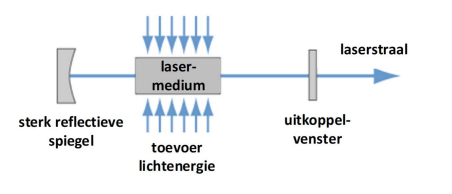
\includegraphics[width=0.6\textwidth]{assets/image77.png}
    \caption{Creeren van een laserstraal door gestimuleerde emissie.}
    \label{fig:creeren_laserstraal.png}
\end{figure}

De laserstraal heeft een paar problemen
\newline
Er wordt veel energie omgezet in warmte en de lichtkwaliteit moet je in
rekening houden.
\newline
Classificatie van lasers:
\begin{itemize}
    \item \textbf{Lasermedium:}
          gas, vast, vloeistof, halfgeleider
    \item \textbf{Golflengte:}
          infrarood, zichtbaar, ultraviolet
    \item \textbf{Aard van de uitgaande straal:}
          continu of gepulst
    \item \textbf{Het vermogen:}
          van milliwatt tot multi-kilowatt
    \item \textbf{Vorm lasercaviteit:}
          langwerpig, rond, ringvormig, fiber en disklasers

    \item \textbf{De pompmethode:}
          elektrisch, optisch
\end{itemize}

Laserlicht kan getransporteerd worden via lucht (met spiegels) of via glasvezel.
Bij een \textbf{fiberlaser} is de glasvezel niet zomaar een transportkabel: de vezel zelf is het lasermedium,
gedoteerd met bijvoorbeeld ytterbium. De laser wordt dus in de vezel opgewekt én erdoor geleid.

\textbf{De golflengte $\lambda$} gaat je laser bepalen.
Kleinere golflengtes laten een kleiner focuspunt toe (dus preciezer werk) maar zijn duurder te maken.
Veel lasertechnologie is recent (vanaf ongeveer het jaar 2000).
Een Nd:YAG-laser ($\lambda \approx \SI{1,06}{\micro m}$) heeft een tienmaal kortere golflengte dan een
CO$_2$-laser ($\lambda \approx \SI{10,6}{\micro m}$) en laat dus preciezer werk toe.

Hieronder zijn alle relevante type lasers voor het bewerken van materialen:
\begin{figure}[ht]
    \centering
    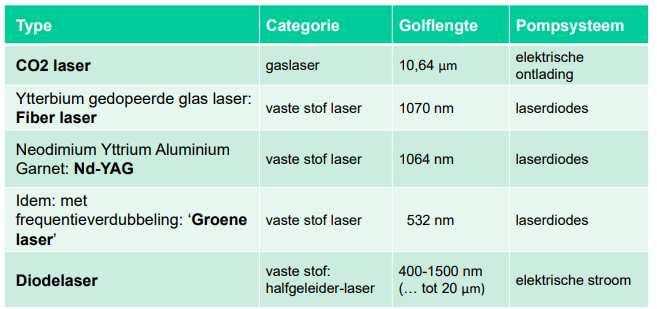
\includegraphics[width=0.8\textwidth]{assets/Type_lasers.png}
    \caption{}
    \label{fig:Type_lasers.png}
\end{figure}

\subsection{Absorptie van laserlicht}

\begin{wrapfigure}[14]{r}{0.52\textwidth}
    \centering
    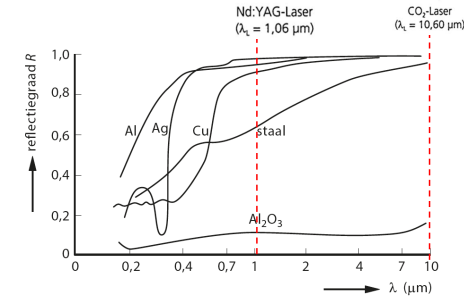
\includegraphics[width=\linewidth]{assets/Reflecteren in functie van de golflengte.png}
    \caption{}
    \label{fig:Reflecteren in functie van de golflengte.png}
\end{wrapfigure}
\FloatBarrier

Je wilt zoveel mogelijk van de laserenergie laten absorberen door het werkstuk.
$R+T+A=1$ met R = reflectie, T = transmissie en A = absorptie.
Je wilt dus een hoge A hebben.

In de figuur zie je dat staal ongeveer 90\% van een CO$_2$-laser reflecteert, terwijl een YAG-laser
er maar zo'n 50\% van reflecteert.
Vroeger loste men dat op door de CO$_2$-laser met enorm grote vermogens te gebruiken, zodat er toch genoeg
energie geabsorbeerd werd.

Die verschillen in absorptie komen door de kristal- en moleculaire structuur van het materiaal:
die bepaalt welke golflengtes het materiaal kan opnemen.

\begin{figure}[ht]
    \centering
    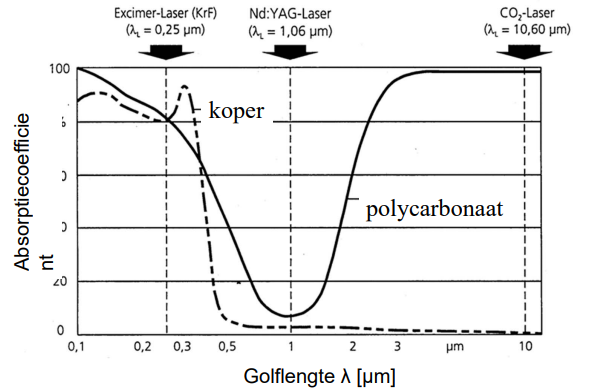
\includegraphics[width=0.5\textwidth]{assets/Absorptie van polycarbonaat.png}
    \caption{}
    \label{fig:Absorptie van polycarbonaat.png}
\end{figure}

Bij kunststoffen zoals polycarbonaat zie je het omgekeerde: een CO$_2$-laser wordt bijna volledig geabsorbeerd,
terwijl een YAG-laser er grotendeels doorheen gaat of gereflecteerd wordt.
Voor die toepassing gebruik je dus liever een CO$_2$-laser.

\subsubsection{Kwaliteit van de laserstraal}
\textbf{Het BPP (Beam Parameter Product)} is een maat voor de kwaliteit van een laserstraal.
\frm{BPP (Beam Parameter Product)}{BPP = w_0 \cdot \dfrac{\theta}{2}}{waarbij $BPP$ het beam parameter product is [\si{mm.mrad}], \(w_0\) de straal van de bundeltaille (het focuspunt) [\si{mm}] en $\theta$ de volledige divergentiehoek [\si{mrad}].}
Hoe kleiner het BPP, hoe beter de bundelkwaliteit: je kunt de straal dan tot een kleiner punt focusseren
zonder dat hij daarna snel uitwaaiert.

Je moet je laser dus focussen als je materiaal wilt bewerken,
en die focusafstand moet precies kloppen; anders krijg je een groter focuspunt en dus minder intensiteit.

\begin{figure}[ht]
    \centering
    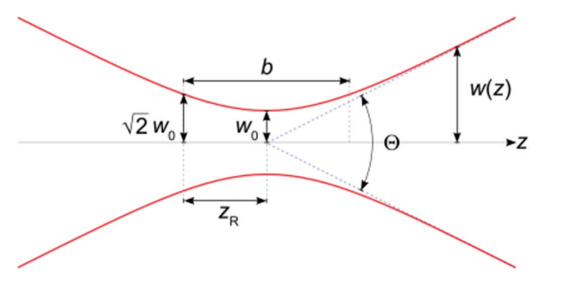
\includegraphics[width=0.5\textwidth]{assets/Kwaliteit laserstraal.png}
    \caption{}
    \label{fig:Kwaliteit laserstraal.png}
\end{figure}

\textbf{Het intensiteitsprofiel van een laserstraal}
Een ideale laser zou een perfecte cilinder met overal dezelfde intensiteit zijn.
In de praktijk is dat niet zo: de intensiteit volgt een \emph{gaussiaans} profiel, het felst in het midden
en afnemend naar de rand toe.

\frm{Gaussiaans intensiteitsprofiel}{I(r) = I_0\,e^{-2r^2/w_0^2}}
{waarbij $I(r)$ de intensiteit is op afstand $r$ van de as [\si{W/mm^2}], $I_0$ de maximale intensiteit
    in het midden van de bundel [\si{W/mm^2}], $r$ de radiale afstand [\si{mm}] en $w_0$ de bundelstraal [\si{mm}].
    Per afspraak is $w_0$ precies de straal waar de intensiteit gezakt is tot $I_0/e^2$ (ongeveer 13,5\% van het maximum).}

\begin{figure}[ht]
    \centering
    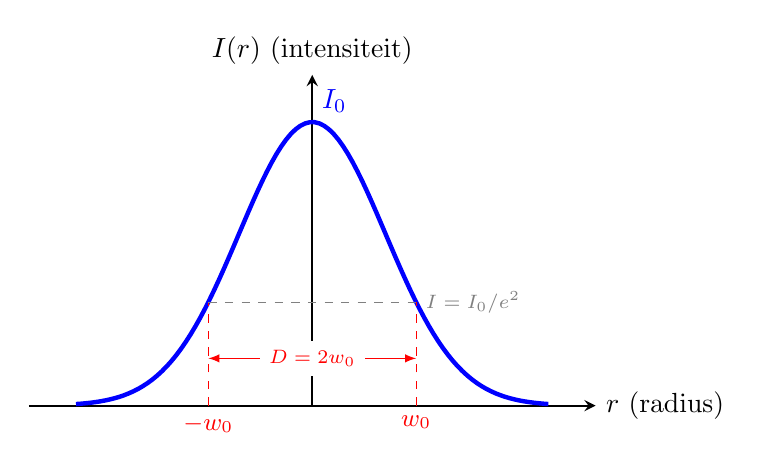
\begin{tikzpicture}[scale=1.2]
        % Assen
        \draw[thick,->,>=stealth] (-3,0) -- (3,0) node[right] {$r$ (radius)};
        \draw[thick,->,>=stealth] (0,0) -- (0,3.5) node[above] {$I(r)$ (intensiteit)};

        % Gaussiaanse curve (parabolische vorm nabij de top)
        \draw[ultra thick, blue, domain=-2.5:2.5, samples=100] plot (\x, {3*exp(-\x*\x/1.2)});

        % Annotaties
        \node[anchor=south west, blue] at (0,3) {$I_0$};

        % Bundelstraal w0 aanduiding
        % Bij x = 1.1 is de waarde ongeveer I0/e^2
        \draw[dashed, red] (-1.1, 0) -- (-1.1, {3*exp(-1.1*1.1/1.2)}) node[below, pos=0, font=\small] {$-w_0$};
        \draw[dashed, red] (1.1, 0) -- (1.1, {3*exp(-1.1*1.1/1.2)}) node[below, pos=0, font=\small] {$w_0$};
        \draw[<->, red, >=latex] (-1.1, 0.5) -- (1.1, 0.5) node[midway, fill=white, font=\scriptsize] {$D = 2w_0$};

        % Niveau I0/e^2
        \draw[dashed, gray] (-1.1, {3*exp(-1.1*1.1/1.2)}) -- (1.1, {3*exp(-1.1*1.1/1.2)}) node[right, font=\scriptsize] {$I = I_0/e^2$};

    \end{tikzpicture}
    \caption{Parabolische/Gaussiaanse intensiteitsverdeling van een laserbundel op het focuspunt.}
    \label{fig:laser_focus_intensity}
\end{figure}

Voor een ideaal gaussiaans profiel geldt:
\[BPP = \frac{\lambda}{\pi}\]
met $\lambda$ de golflengte van de laser. Dit is de theoretisch best haalbare waarde.

\textbf{Een kleinere golflengte $\lambda$ geeft dus een betere bundelkwaliteit van de laserstraal.}

Om de bundel te focussen gebruik je een lens met brandpuntsafstand \(f\).
De bundel wordt dan samengeknepen tot een taille met straal \(w_0\):
\[w_0 = \frac{4 \lambda f}{\pi D}\]
met \(D\) de bundeldiameter op de lens. Een korte brandpuntsafstand en een brede invallende bundel
geven dus het kleinste focuspunt. Kleine hoogteverschillen tussen lens en werkstuk maken daardoor
een groot verschil in de bereikte intensiteit.

\begin{figure}[htbp]
    \centering
    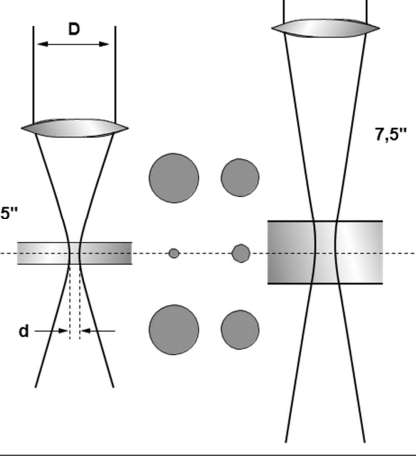
\includegraphics[width=0.3\textwidth]{assets/Laserfocussen.png}
    \caption{Laserfocussen met verschillende focusafstanden \(f\).}
    \label{fig:Laserfocussen.png}
\end{figure}
\FloatBarrier

De $w_0$ kun je meten met warmtecamera's die het intensiteitsprofiel van de laser opnemen.
Daaruit bereken je dan het BPP.

\subsection{Toepassingen}
\begin{itemize}
    \item \textbf{Snijden}: Het materiaal wordt lokaal gesmolten of verdampt door de hoge energiedichtheid, vaak ondersteund door een snijgas om de smelt te verwijderen.
    \item \textbf{Lassen}: Het verbinden van twee delen door ze op het contactvlak te smelten, wat resulteert in een smalle, diepe lasnaad met minimale thermische vervorming.
    \item \textbf{Boren}: Gebruik van korte laserpulsen met zeer hoge intensiteit om materiaal te verdampen en zo nauwkeurige gaten te creëren.
    \item \textbf{Oppervlaktebehandeling}: Aanpassen van de textuur of chemie van de toplaag, zoals het reinigen van oppervlakken of het creëren van specifieke ruwheidspatronen.
    \item \textbf{Harden}: Het lokaal verhitten van staal boven de kritische temperatuur,
          gevolgd door zelfafschrikking via de omringende koude massa, om de slijtvastheid te verhogen.
          Zo kun je de flanken van tandwielen harden terwijl de kern taai blijft.
          Bij laserharden krijg je veel minder vervorming dan bij harden in een oven, omdat je alleen lokaal opwarmt.
    \item \textbf{Cladding}: Een laag van een ander materiaal (poeder of draad) op het werkstuk smelten om eigenschappen zoals corrosiebestendigheid of hardheid te verbeteren.
    \item \textbf{Solderen}: Het smelten van een toevoegmateriaal met de laser om een verbinding te maken, waarbij het basismateriaal zelf niet smelt (soldeerverbinding).
\end{itemize}

Afhankelijk van de toepassing moet je het BPP en het vermogen aanpassen.

\subsection{Machinegestuurde lasers (NC-lasers)}
Lasers worden vandaag NC-gestuurd, waardoor je alle parameters tijdens de bewerking kunt bijsturen.
De computer focusseert de laser zelf, past de snelheid dynamisch aan afhankelijk van de snede
(trager in bochten, sneller op rechte stukken) en regelt het vermogen mee.
\begin{figure}[htbp]
    \centering
    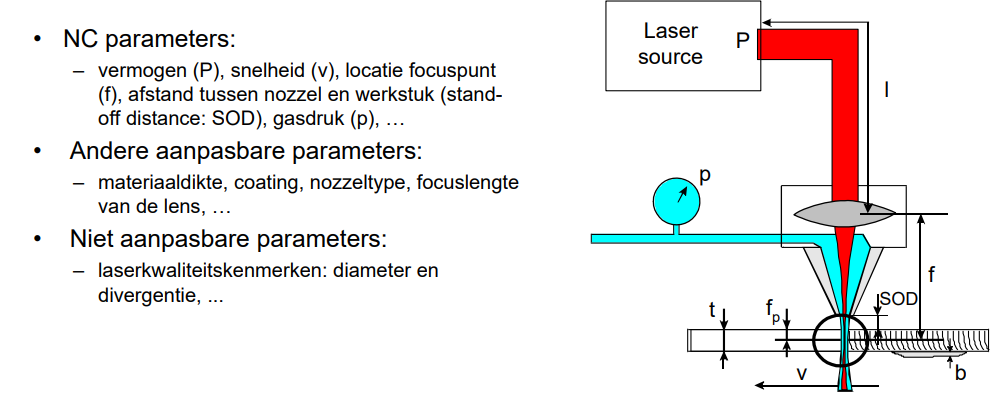
\includegraphics[width=1\textwidth]{assets/NC-lasers.png}
    \caption{NC laser snijmachine}
    \label{fig:NC-lasers.png}
\end{figure}

\textbf{Belangrijke parameters bij lasersnijden}

\textbf{Lasersmeltsnijden}: er wordt een inert snijgas (stikstof, argon) toegevoegd dat de smelt wegblaast.
Omdat het gas inert is, treedt er geen oxidatie op en blijft de snijkant blank; het gas koelt bovendien mee af.

\textbf{Laserbrandsnijden}: je doet net het omgekeerde en gebruikt zuurstof als snijgas.
Het metaal verbrandt dan mee, wat extra warmte levert en het proces versnelt, maar je krijgt wel een
geoxideerde snijkant.

In beide gevallen is het belangrijk om het verwijderde materiaal (smelt) weg te blazen met het snijgas.

\subsubsection{Toepassingen}
Lasersnijden is snel en nauwkeurig en kan enorm kleine dingen maken.
\begin{figure}[htbp]
    \centering
    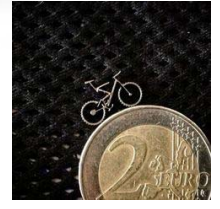
\includegraphics[width=0.4\textwidth]{assets/Kleinefiguurdoorlasersnijden.png}
    \caption{Toepassingen van lasersnijden in verschillende industrieën}
    \label{fig:Laser_toepassingen.png}
\end{figure}
\FloatBarrier

Lasersnijden kan zowel op grote als op kleine schaal. Grote platen staal worden er bijvoorbeeld mee gesneden
voor de auto-industrie.

\subsubsection{Nadelen}
\begin{itemize}
    \item \textbf{Dross}: Tijdens het snijden kan er een ophoping van gesmolten materiaal aan de onderkant van het snijvlak ontstaan, wat resulteert in een ruwe afwerking die vaak nabewerking vereist.
    \item \textbf{Verbrandingsdefecten (burning)}: Bij een te lage snijsnelheid, bijvoorbeeld bij kunststoffen, kan overmatige hitte leiden tot verbranding of verkoling langs de snijranden, wat de kwaliteit van het eindproduct vermindert.
    \item \textbf{Onvolledige penetratie}: Bij dikkere materialen kan de laserstraal niet volledig door het materiaal heen dringen, wat resulteert in onvolledige sneden die opnieuw bewerkt moeten worden.
    \item \textbf{Aanhechting van gesmolten materiaal}: Bij brandsnijden aan hoge snijsnelheden kan gesmolten materiaal aan de snijkant blijven plakken, wat leidt tot onregelmatige randen en mogelijke structurele zwaktes in het gesneden onderdeel.
\end{itemize}

\begin{warningbox}[EXAMEN CHECKLIST: NIET-CONVENTIONELE BEWERKINGEN]
    \begin{itemize}
        \item \textbf{EDM vs. ECM}: Ken het fundamentele verschil (thermisch vs. chemisch) en de vloeistof (diëlektricum vs. elektrolyt).
        \item \textbf{EDM Fases}: Begrijp de cyclus: ontbranding $\to$ ontlading (plasma) $\to$ implosie (swarf afvoer).
        \item \textbf{EDM Slijtage}: Begrijp waarom de elektrode wel slijt bij EDM (ionenbombardement) maar niet bij ECM (kathode neemt anode (werkstuk) materiaal op).
        \item \textbf{ECM Afname}: Leg uit waarom de afnamesnelheid afhangt van de stroom ($I$) en de atoommassa, niet van de hardheid van het materiaal.
        \item \textbf{Laser}: Begrijp de energiebalans ($A+R+T=1$), het BPP en waarom de golflengte cruciaal is voor de materiaalkeuze.
        \item \textbf{Ultrasoon}: Weet dat dit ideaal is voor brosse materialen (keramiek) door microscheur-initiatie.
    \end{itemize}
\end{warningbox}

\chapter{Scheiden}

\begin{conceptbox}[Knippen vs. Ponsen]
    \begin{itemize}
        \item \textbf{Knippen}: Scheiden langs een open lijn (meestal recht) met twee langs elkaar bewegende messen.
        \item \textbf{Ponsen}: Scheiden langs een gesloten contour met behulp van een stempel en een matrijs.
    \end{itemize}
\end{conceptbox}

Bij scheiden ga je knippen of ponsen. Hierbij ontstaan er \emph{geen} spanen:
het materiaal wordt afgeschoven tot het breekt.
Het uitgesneden deel blijft daardoor bruikbaar, in tegenstelling tot bij verspanen.
\newline
\section{Ponsen en knippen}
Bij \textbf{ponsen} maak je met een gesloten profiel een gat in een plaat.
\newline
Bij \textbf{knippen} scheid je je materiaal langs een open (meestal rechte) lijn.
\newline
Zolang je onder de vloeigrens blijft veert het materiaal gewoon terug; pas bij plastische vervorming
verandert de vorm blijvend. Daarvoor heb je een afschuifkracht nodig.
\newline
\frm{Afschuifkracht bij ponsen}{\ensuremath{F_{th} = \tau_{max} \cdot L \cdot s_0}}{Waarbij
    \(\!F_{th}\!\) de afschuifkracht is [\si{N}], \(\tau_{max}\) de maximale schuifspanning [\si{N/mm^2}],
    \(L\) de omtrek van het profiel [\si{mm}] en \(s_0\) de plaatdikte [\si{mm}].}

Het materiaal schuift af tot het doorbreekt; dan is je stuk gescheiden.

\begin{figure}[ht]
    \centering
    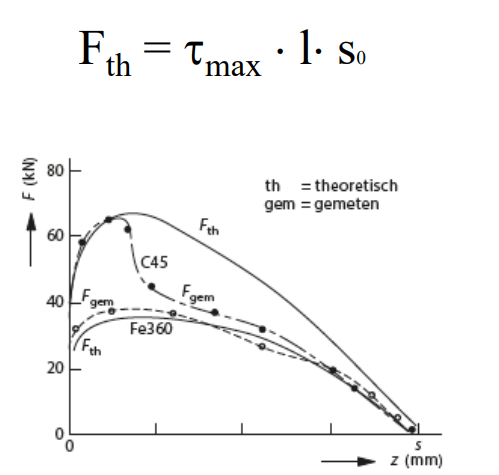
\includegraphics[width=0.45\textwidth]{assets/Kracht-wegdiagram van Ponsen.png}
    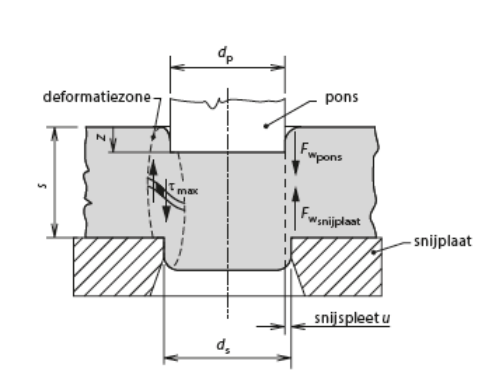
\includegraphics[width=0.45\textwidth]{assets/Het Ponsprocess.png}
    \caption{}
    \label{fig:Kracht-wegdiagram van Ponsen.png}
\end{figure}
\FloatBarrier
In de grafiek zie je de kracht eerst stijgen: dat is de opbouw van de schuifkracht tot de piekbelasting.
Daarna daalt de kracht weer, omdat het materiaal begint te breken en de doorsnede die nog draagt kleiner wordt.
De $z$-waarde is de weg die de stempel aflegt tot het materiaal doorbreekt.

Bij knippen en ponsen heb je drie fases:
\begin{enumerate}
    \item \textbf{Elastische vervorming}: Het materiaal ondergaat een tijdelijke vervorming die verdwijnt wanneer de kracht wordt verwijderd.
    \item \textbf{Plastische vervorming}: Het materiaal begint permanent te vervormen zodra de vloeigrens is overschreden.
    \item \textbf{De scheidingsfase}: Uiteindelijk bereikt het materiaal zijn breekpunt, wat resulteert in het scheiden van het materiaal.
\end{enumerate}

De vorm en de kwaliteit van de snede hangen af van de breedte van de snijspleet.
\begin{figure}[ht]
    \centering
    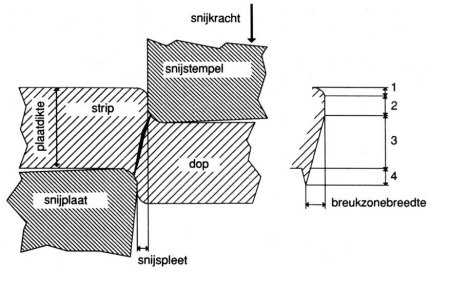
\includegraphics[width=0.55\textwidth]{assets/image80.png}
    \caption{Afschuiving door knippen}
    \label{fig:image80.png}
\end{figure}



\subsection{Knippen}
Knippen is een spaanloze bewerking.
In plaats van een spaanhoek heb je hier een snijhoek $\gamma$ en een vrijloophoek $\alpha$.
Een voorbeeld van een knipmachine is een guillotineschaar.

\textit{Zelfde soort hoeken als bij verspanen, maar zonder spaanvorming.}

\frm{Schuifkracht bij knippen}
{\ensuremath{F = 0.5 \cdot \dfrac{s^2}{\tan\varepsilon} \cdot \tau}}
{waarbij \(F\) de afschuifkracht is [\si{N}], \(s\) de plaatdikte [\si{mm}], \(\varepsilon\) de snijhoek [$^\circ$] en \(\tau\) de schuifspanning van het materiaal [\si{N/mm^2}].}

De \textbf{snijspleet} is de afstand tussen het mes en het tegenmes.
Is die niet goed ingesteld, dan krijg je slechte sneden: te klein geeft extra kracht en slijtage,
te groot geeft bramen en een omgeplooide rand.
Dat is ook de reden waarom versleten scharen slechte sneden geven.

\begin{figure}[htbp]
    \centering
    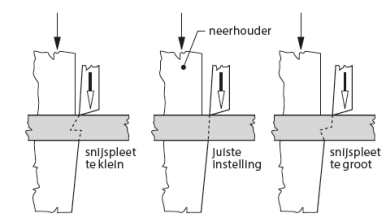
\includegraphics[width=0.6\textwidth]{assets/snijspleetbelang.png}
    \caption{Het belang van de juiste snijspleet bij knippen}
    \label{fig:snijspleetbelang.png}
\end{figure}

Nog voorbeelden van knipmachines zijn:
\begin{itemize}
    \item \textbf{strokenschaar} - Een knipmachine speciaal ontworpen voor het verwerken van langwerpige stroken metaal.
          Deze machines zijn ideaal voor het afkorten van platen tot breedte en maken lange, rechte sneden met hoge precisie.

    \item \textbf{rolschaar} - Een knipmachine die werkt met twee tegenover elkaar geplaatste, ronddraaiende messen.
          Hierdoor wordt een continue knipvorming gecreëerd wat bijzonder geschikt is voor het produceren van lange rechte sneden en het verwerken van dikke platen met minder krachtinspanning.

    \item \textbf{figuurschaar} - Een geavanceerde knipmachine in staat om complexe vormen en contouren te snijden.
          Deze machines worden vaak CNC-gestuurd en kunnen zowel rechte als gebogen sneden maken, ideaal voor het produceren van op maat gemaakte onderdelen en profielen.
\end{itemize}


\subsection{Ponsen}
Ponsen is ook een spaanloze bewerking. Een simpel voorbeeld is een perforator.

\frm{Eerste formule Schuifkracht bij ponsen}{\ensuremath{F = s_0 \cdot l \cdot \tau}}
{waarbij \(F\) de afschuifkracht is [\si{N}], \(s_0\) de plaatdikte [\si{mm}], \(l\) de omtrek van het profiel [\si{mm}] en \(\tau\) de schuifspanning van het materiaal [\si{N/mm^2}].}

Bij ponsen snijdt de volledige omtrek in één keer aan. Er is dus nauwelijks geleidelijke opbouw:
je krijgt meteen een indrukking en een snel oplopende schuifspanning, en dus een hoge piekkracht.

\begin{figure}[htbp]
    \centering
    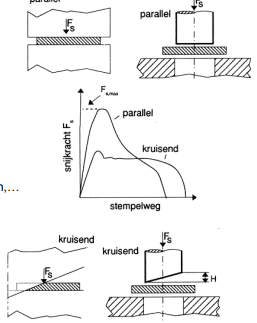
\includegraphics[width=0.3\textwidth]{assets/Schuifspanningen bij Ponsen.png}
    \caption{Ponsen proces met de verschillende fases}
    \label{fig:Ponsen proces.png}
\end{figure}
\FloatBarrier

De eerste formule is een benadering.
Een betere formule is:
\frm{Tweede formule schuifkracht bij ponsen}{\ensuremath{F = 1{,}6 \cdot y_s \cdot s_0 \cdot l \cdot k_s}}
{waarbij \(F\) de afschuifkracht is [\si{N}], \(y_s\) een correctiefactor voor de snijspleet [-],
\(s_0\) de plaatdikte [\si{mm}], \(l\) de omtrek van het profiel [\si{mm}] en \(k_s\) de specifieke
snijkracht [\si{N/mm^2}].}

De factor 1,6 houdt rekening met de gereedschapsslijtage: een botte stempel vraagt tot 60\% meer kracht
dan een scherpe.

\textbf{$k_s$ de specifieke snijkracht}
\newline
De specifieke snijkracht \(k_s\) is de kracht die nodig is per mm$^2$ te snijden doorsnede.
Ze wordt uitgedrukt in \si{N/mm^2} en hangt af van het materiaaltype en de plaatdikte.
\[
    k_s = X_f \cdot R_m
\]
met \(X_f\) de snijfactor en \(R_m\) de treksterkte van het materiaal.



\subsection{Fijnstancen}

\begin{conceptbox}[Fijnstansen]
    Fijnstansen is een precisie-ponsproces waarbij de snijspleet extreem klein is ($<1\%$ van de plaatdikte)
    en het materiaal volledig wordt vastgeklemd. Dit resulteert in een volledig glad snijvlak over de hele dikte,
    zonder de typische breukzone van normaal ponsen.
\end{conceptbox}

Fijnstansen is snijden en ponsen met een heel kleine snijspleet, rond 0,01 tot 1 mm
(minder dan 1\% van de plaatdikte).
Bij normaal ponsen en knippen is er speling rond de stempel, waardoor de plaat mee omhoog
getrokken kan worden en er een scheurzone ontstaat.

Bij fijnstansen is die speling er niet meer.
De plaat wordt volledig vastgeklemd tussen een ringtandhouder en een tegenhouder,
en de stempel wordt daardoor heel precies geleid.
De snijspleet is klein én overal constant.

\begin{figure}[htbp]
    \centering
    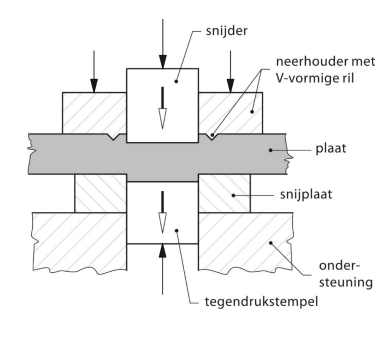
\includegraphics[width=0.3\textwidth]{assets/Fijnsnijden.png}
    \caption{}
    \label{fig:Fijnsnijden.png}
\end{figure}
\FloatBarrier

Het is duurder, maar het snijvlak is over de volledige plaatdikte glad, zonder de typische breukzone.
De kwaliteit is beter dan bij lasersnijden en normaal ponsen.

\subsection{Volgsnijstempel}

\begin{conceptbox}[Volgsnijstempel]
    Bij volgsnijstempel heb je een soort lopende band van ponsen.
    Stel je wilt een sleutel maken. De plaat schuift stap voor stap door en bij elke stap voert
    een andere stempel één bewerking uit: eerst de gaten, dan de contour, dan het afsnijden.
    De plaat blijft doorlopen, zodat je in hoog tempo veel producten maakt.
\end{conceptbox}

Je verdeelt de verschillende operaties over verschillende stempels.
Die stempels dienen niet alleen om te ponsen: ze kunnen het product ook buigen, dieptrekken of vormen.

Deze techniek wordt gebruikt wanneer je grote aantallen van een product moet maken.
De stempels (gemaakt uit hard staal met wolframcarbide) zijn duur maar je kunt er wel enorm snel mee werken.

\begin{examenbox}
    Als je een werkvoorbereiding moet maken voor een vlak deel dat licht gebogen is,
    en je moet er veel van maken, dan antwoord je \textbf{volgsnijstempel}.
    Je kunt er zowel mee snijden als mee vormen.
\end{examenbox}

\begin{warningbox}[Examenvraag]
    \textbf{Hoe zou je de geleiders maken voor een volgsnijstempel?}

    Met draadvonken kun je heel precies openingen uit hardmetaal maken in dezelfde vorm als de stempel.
    Je maakt de toppen van de geleiders uit keramiek zodat ze niet slijten.
\end{warningbox}

\subsection{Revolvermachine}

Je kunt computergestuurd ponsen op een grote aluminium plaat.
De plaat beweegt onder de pons door langs de $x$- en $y$-as, terwijl de revolverkop het juiste
ponsgereedschap in positie draait.
Dit gaat enorm snel.
Het is sneller dan een lasersnijmachine dus als je grote aantallen moet maken is dit ideaal.

\subsection{Knabbelen}

Bij knabbelen ga je rond een contour ponsen om iets uit te knippen.
Afhankelijk van de stapgrootte tussen de ponsen krijg je een grovere of fijnere rand.
Dit is enorm snel, rond 10 slagen per seconde.

\begin{figure}[htbp]
    \centering
    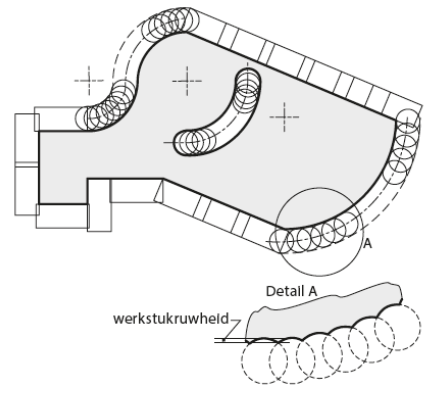
\includegraphics[width=0.3\textwidth]{assets/Ruw oppervlakte Knappelen.png}
    \caption{}
    \label{fig:Knabbelen.png}
\end{figure}
\FloatBarrier

De pons kun je combineren met verschillende vormen: cirkel, vierkant, driehoek enz.

\section{Mechanisch scheiden door verspanen}

Bij mechanisch scheiden neem je materiaal weg door te verspanen.
De structuur van je materiaal verandert daarbij niet (geen thermisch aangetaste zone).
Je hebt verschillende technieken:
\begin{itemize}
    \item \textbf{Zagen}: Gebruik van een zaagblad met tanden om materiaal te verwijderen door middel van een snijbeweging.
    \item \textbf{Schuren}: Verwijderen van materiaal met schuurpapier of schuurbanden door wrijving.
    \item \textbf{Slijpen}: Gebruik van een slijpschijf om materiaal te verwijderen en een glad oppervlak te creëren.
    \item \textbf{Polijsten}: Fijnere afwerking van oppervlakken door gebruik van polijstmiddelen en doeken.
    \item \textbf{Boren}: Creëren van ronde gaten in materialen met behulp van een boor.
\end{itemize}

\section{Fysische scheiding}
Bij fysische scheiding ga je materiaal wegnemen door fysische processen.
Je hebt opnieuw verschillende technieken:

\begin{itemize}
    \item \textbf{Brandsnijden}: Metaal snijden door verbranding met behulp van een zuurstofstraal.
          Het materiaal wordt verhit tot boven de ontbrandingstemperatuur en vervolgens wordt zuurstof toegevoegd
          om het metaal te oxideren en weg te blazen.\\

          Als je \textbf{te weinig zuurstof} gebruikt krijg je \textbf{aanhechting van gesmolten materiaal.}\\

          Als je \textbf{te veel zuurstof} gebruikt krijg je een \textbf{ruwe rand en een te grote snijholte.}
    \item \textbf{Draadvonken}: Gebruik van elektrische vonken tussen een elektrode en het werkstuk om materiaal te verwijderen.
    \item \textbf{Stralen}: Gebruik van abrasieve deeltjes om materiaal te verwijderen of oppervlakken te reinigen.
    \item \textbf{Laser snijden}: Gebruik van een geconcentreerde laserstraal om materiaal te smelten of te verdampen.
    \item \textbf{Waterstraalsnijden}: Gebruik van een hogedruk waterstraal om materiaal te snijden zonder thermische effecten.
    \item \textbf{Plasmasnijden}: Gebruik van een plasmaboog om metaal te snijden door het te verhitten en te smelten.
          Plasma is een vlam van geïoniseerd gas die extreem heet is (tot \SI{20000}{\degreeCelsius}).
\end{itemize}

\begin{figure}[htbp]
    \centering
    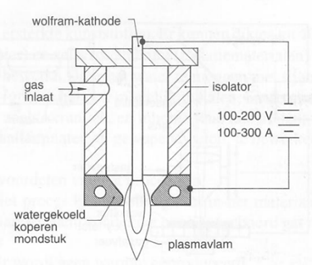
\includegraphics[width=0.3\textwidth]{assets/plasmasnijden.png}
    \caption{Plasmasnijden proces}
    \label{fig:Plasmasnijden.png}
\end{figure}

\begin{engtable}[
        caption = {Vergelijking van scheidingsprocessen},
        label = {tab:scheidingsprocessen},
    ]{
        colspec = {l X[l] l X[l] c c},
        width = \textwidth,
        cells = {font=\small},
        row{1} = {font=\bfseries},
    }
    Processen & Toepassing & Snelheid & {Voor- en nadelen} & {Nauwk.\\(mm)} & {WBZ\\(mm)} \\
    Knippen & Plaat 0,2--10mm & lengte/knip & {+ grote lengten \\ -- bramen} & $>0,1$ & -- \\
    Ponsen & Plaat 0,2--10mm & $\le$ 30 sl/s & {+ massa \\ -- bramen} & $>0,1$ & -- \\
    Knabbelen & Plaat 0,2--10mm & $\le$ 0,1 m/s & {+ massa/kl. prod. \\ + contouren \\ -- bramen/ruw} & 0,1 & -- \\
    Uitsnijden & Plaat 0,2--3mm & $\le$ 30 sl/s & {+ massa \\ + kleine prod.} & 0,05 & -- \\
    Zagen & Plaat/buis/staf $>1$mm & $\le$ 0,05 m/s & {+ enk. st./massa \\ -- bramen} & $>0,3$ & -- \\
    Doorslijpen & Harde mat. (tot 90mm) & ? & {+ enk. st./massa \\ -- bramen} & 0,05 & $<0,1$ \\
    Omtrekfrezen & Platen (tot 12mm) & ? & {+ glad contour \\ -- enk. stuks} & 0,05 & -- \\
    {Waterstraal-\\snijden} & Plaat/buis/staf $>1$mm & $\le$ 0,08 m/s & {+ flexibel/geen WBZ \\ + enk. st./series \\ -- lawaai} & 0,1 & -- \\
    Brandsnijden & Staal $>500$mm, buis & $\le$ 0,05 m/s & {+ flexibel \\ + enk. st./series \\ -- lawaai/WBZ} & $>0,5$ & $>2$ \\
    Plasmasnijden & Geleidende mat. $>10$mm & $\le$ 0,2 m/s & {+ flexibel \\ + enk. st./series \\ -- WBZ} & 0,5 & $>1$ \\
    Lasersnijden & Plaat/buis/prof. $\le$ 5mm & $\le$ 0,2 m/s & {+ flexibel/kwaliteit \\ + enk. st./series \\ + kleine WBZ} & 0,2 & $>0,1$ \\
    Draadvonken & Harde geleidende mat. & $\le$ 0,7 mm$^2$/s & {+ flexibel \\ + enk. st./series \\ + kwaliteit} & 0,05 & $<0,1$ \\
\end{engtable}

Deze tabel is enorm belangrijk, want hij kan hierover vragen stellen: welke van deze technieken
is het snelst, het goedkoopst, het nauwkeurigst enzovoort.

Je ziet dat heel veel technieken die we al gezien hebben hier terugkomen.
Dat maakt dit hoofdstuk vooral een goede herhaling.

\begin{warningbox}[EXAMEN CHECKLIST: SCHEIDEN]
    \begin{itemize}
        \item \textbf{Ponsen \& Knippen}: Begrijp het proces (elastisch $\to$ plastisch $\to$ breuk) en de invloed van de snijspleet.
        \item \textbf{Schuifkracht}: Ken de formule $F = \tau \cdot L \cdot s_0$ en weet hoe de snijhoek de kracht vermindert.
        \item \textbf{Fijnstansen}: Leg uit waarom de precisie hier veel hoger is en ken de noodzaak voor een drievoudige krachtwerking.
        \item \textbf{Volgsnijstempel}: Begrijp het principe van opeenvolgende bewerkingen in één matrijs voor massaproductie.
        \item \textbf{Brandsnijden}: Weet dat dit een chemisch proces is (oxidatie) en ken de beperkingen (grote TAZ, ruwe rand).
    \end{itemize}
\end{warningbox}

\chapter{Oervormen (Gieten van metalen)}

\begin{conceptbox}[Slink vs. Krimp]
    \begin{itemize}
        \item \textbf{Slink}: Volumevermindering tijdens de faseovergang van vloeibaar naar vast. Dit wordt gecompenseerd door
              \keyterm{opkomers} (voedingsreservoirs).
        \item \textbf{Krimp}: Volumevermindering tijdens de verdere afkoeling van het gestolde metaal naar kamertemperatuur.
              Dit wordt gecompenseerd door de \keyterm{krimptoeslag} op het model.
    \end{itemize}
\end{conceptbox}

\section{Inleiding}

\begin{conceptbox}[Directionele stolling]
    Om slinkholtes te voorkomen, moet het gietstuk zo ontworpen zijn dat de stolling begint bij de dunste delen en eindigt bij de opkomer.
    De opkomer moet als laatste stollen om het krimpend metaal in het gietstuk aan te vullen.
\end{conceptbox}

Bij oervormen ga je een vormloos materiaal (vloeistof, pasta, poeder) in een profiel gieten
en dan laten afkoelen en stollen zodat het zijn vorm behoudt.
In dit hoofdstuk hebben we het vooral over metaalgieten.
Metaalgieten is al eeuwenoud en is toegepast in het oude Rome, China enz.

Je gaat vaak meerdere stukken gieten.
Je hebt ook enorm veel vrijheid in de vorm die je kunt gieten.

De materialen die we kunnen gebruiken:
\begin{itemize}
    \item ferro-materialen: lamellair gietijzer, nodulair gietijzer, gietstaal, enz.
    \item niet-ferro-materialen: aluminiumlegeringen, koperlegeringen, magnesiumlegeringen, titaniumlegeringen, enz.
    \item niet-metalen: kunststoffen, keramiek, composieten, enz.
\end{itemize}

Je hebt dus een grote keuze aan materialen.

\begin{figure}[htbp]
    \centering
    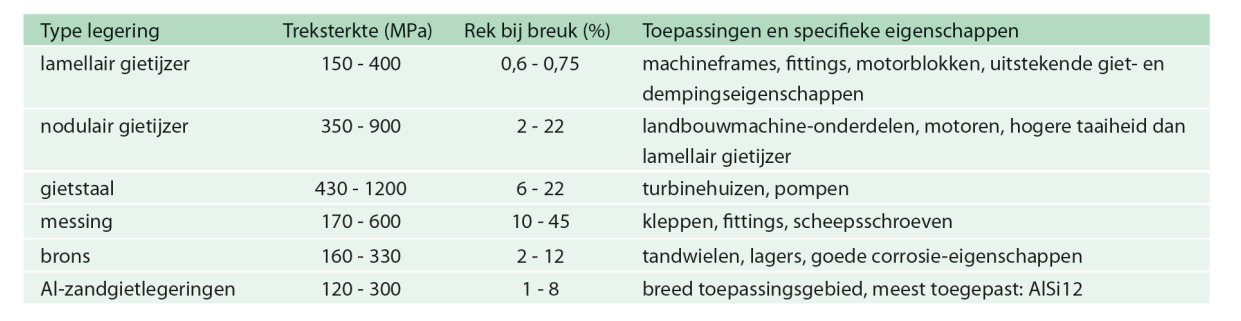
\includegraphics[width=1\textwidth]{assets/Tabel van soorten legeringen die gegoten worden.png}
    \caption{Tabel van soorten legeringen die gegoten worden.}
    \label{fig:Tabel van soorten legeringen die gegoten worden.png}
\end{figure}

De stappen om een gietstuk te maken zijn:
\begin{enumerate}
    \item Smelten van materiaal
    \item Vullen van een vormholte $\to$ afkoeling van het materiaal
    \item Uitnemen van het stuk
\end{enumerate}

\begin{conceptbox}[Volumevermindering bij stollen]
    Volumevermindering door stollen noemt men \belangrijk{slink}. Als die niet aangevuld wordt, ontstaat er
    een \textbf{slinkholte}: een gat in het gietstuk. Je compenseert slink met \textbf{opkomers}:
    extra reservoirs metaal die je aan je gietstuk hangt en die als laatste stollen.\\

    De volumevermindering door het afkoelen noemt men \belangrijk{Krimp}. $\to$ gecompenseerd door krimptoeslag.
    Dit is een extra maat die je aan je gietstuk toevoegt zodat het na afkoeling de juiste maat heeft.

    De krimphoeveelheid hangt af van:
    \begin{itemize}
        \item de geometrie
        \item legering
    \end{itemize}
    Grotere stukken krimpen meer dan kleine stukken.
\end{conceptbox}

\subsection{Maken van een vormholte}
Je hebt twee soorten vormen:
\begin{itemize}
    \item \textbf{Permanente vormen}: Je kunt deze vormen meerdere keren gebruiken. Gemaakt uit metaal.
    \item \textbf{Eenmalige vormen}: Je kunt deze vormen maar één keer gebruiken. Gemaakt uit zand of keramiek.
\end{itemize}
\textbf{Eenmalige vormen:}

Je maakt je vorm uit zand en giet daarin.
Om het stuk eruit te halen breek je het zand weg, en daarmee gaat de vorm verloren.

\textbf{Permanente vormen:}

Je gaat je vorm maken uit metaal.
Je kunt dan spuitgieten, coquillegieten of andere speciale giettechnieken gebruiken.

De keuze hangt af van de smelttemperatuur waarmee je gaat gieten.

\section{Gieten in zand}
Gieten in zand is niet heel precies maar er is geen limiet aan de grootte van het product dat je kunt maken
en het is goedkoop. In de industrie gaan ze dus vaak voor zandgieten en daarna nabewerken om de ruwheid en precisie te verbeteren.
Het zand dat ze gebruiken is niet zomaar zand, maar een mengsel van zand, klei en water dat veel steviger
is dan gewoon zand en zijn vorm houdt na het aanstampen.

\begin{figure}[htbp]
    \centering
    \begin{minipage}[b]{0.48\textwidth}
        \centering
        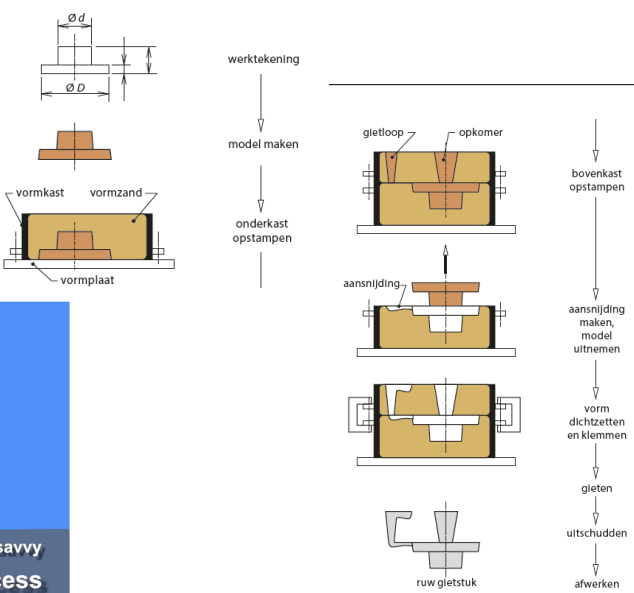
\includegraphics[width=\linewidth]{assets/Zandgieten.png}
    \end{minipage}\hfill
    \begin{minipage}[b]{0.48\textwidth}
        \centering
        \begin{tikzpicture}[node distance=1.6cm, auto,
                block/.style={rectangle, draw, rounded corners, fill=blue!10, text width=12.5em, align=center, minimum height=2.5em},
                line/.style={draw, -Latex, thick}]
            % Nodes
            \node [block] (model) {Model maken\\(groter voor krimp)};
            \node [block, below of=model] (zand) {Model in zand stampen};
            \node [block, below of=zand] (kanalen) {Gietloop \& opkomer maken};
            \node [block, below of=kanalen] (aansnede) {Aansnede maken \& model verwijderen};
            \node [block, below of=aansnede] (gieten) {Metaal gieten};
            \node [block, below of=gieten] (afkoelen) {Afkoelen};
            \node [block, below of=afkoelen] (verwijderen) {Zand, gietloop \& opkomer verwijderen};
            \node [block, below of=verwijderen] (nabewerken) {Nabewerken};

            % Paths
            \path [line] (model) -- (zand);
            \path [line] (zand) -- (kanalen);
            \path [line] (kanalen) -- (aansnede);
            \path [line] (aansnede) -- (gieten);
            \path [line] (gieten) -- (afkoelen);
            \path [line] (afkoelen) -- (verwijderen);
            \path [line] (verwijderen) -- (nabewerken);
        \end{tikzpicture}
        \par\smallskip\small (b) Stappen in zandgieten
    \end{minipage}
    \caption{(a) Zandgietenproces; (b) Schematische workflow van de belangrijkste stappen bij zandgieten.}
    \label{fig:Zandgieten proces.png}
\end{figure}
\FloatBarrier

Het model moet iets groter zijn dan het uiteindelijke product om krimp te compenseren.
Nadat het model in het zand is gestampt, wordt er een aansnede gemaakt in de bovenkant van de zandvorm zodat het model verwijderd
kan worden. Na het gieten en afkoelen wordt het zand verwijderd en worden de gietloop en opkomer afgebroken.

\begin{conceptbox}[Gietloop en opkomer]
    De \textbf{gietloop} is het kanaal waardoor het gesmolten metaal in de vormholte stroomt.
    Het ontwerp van de gietloop is cruciaal om een gelijkmatige vulling van de vorm te garanderen en om turbulentie te minimaliseren,
    wat kan leiden tot defecten in het gietstuk.\\

    De \textbf{opkomer} is een extra reservoir dat is verbonden met de vormholte en dient als een bron van extra metaal tijdens het stollingsproces.
    Dit helpt om volumevermindering door \textbf{slink} te compenseren en voorkomt het ontstaan van holtes of insluitingen in het uiteindelijke gietstuk.
    De opkomer helpt ook de operator te laten zien of het gietstuk volledig is gevuld.
\end{conceptbox}

\subsection{Problemen bij gieten}
\begin{conceptbox}[Slink, krimp en lossing]
    \begin{enumerate}
        \item \textbf{Slink}: Volumevermindering door stollen. Gecompenseerd door opkomers.
        \item \textbf{Krimp}: Volumevermindering door afkoelen. Gecompenseerd door krimptoeslag.
        \item \textbf{Lossing}: Het proces van het verwijderen van het gietstuk uit de vorm.
              Belangrijk om te zorgen dat het gietstuk niet beschadigd raakt tijdens het verwijderen.
    \end{enumerate}
\end{conceptbox}

Om deze dingen te voorkomen zetten we opkomers. Materialen kunnen complexe geometrie hebben.
Soms moet je dus meerdere opkomers zetten zodat de vorm overal goed gevuld wordt.

\begin{figure}[ht]
    \centering
    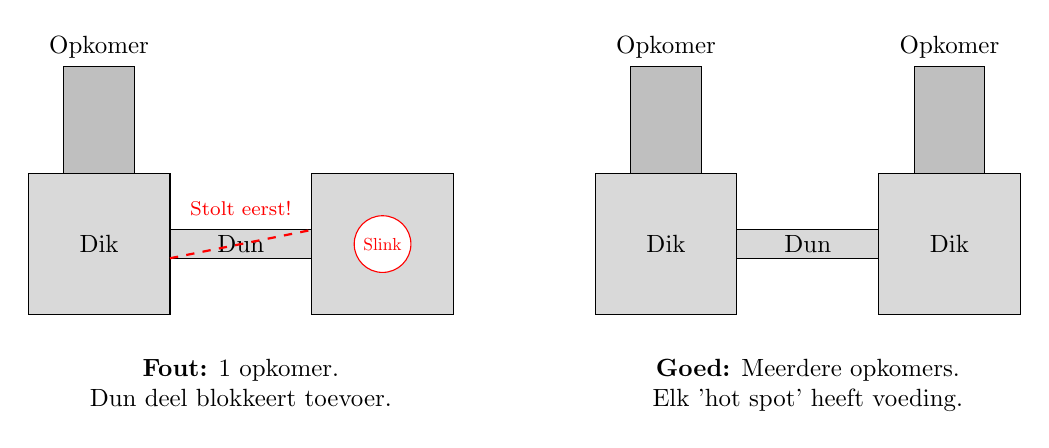
\begin{tikzpicture}[scale=0.9, every node/.style={transform shape}]
        % Bad scenario
        \begin{scope}[xshift=0cm]
            % Casting parts 
            \draw[fill=gray!30] (0,0) rectangle (2,2) node[midway] {Dik};
            \draw[fill=gray!30] (2,0.8) rectangle (4,1.2) node[midway] {Dun};
            \draw[fill=gray!30] (4,0) rectangle (6,2) node[midway] {Dik};

            % Riser on left only
            \draw[fill=gray!50] (0.5,2) -- (0.5,3.5) -- (1.5,3.5) -- (1.5,2);
            \node[above] at (1,3.5) {Opkomer};

            % Solidification/Defect
            \draw[dashed, red, thick] (2,0.8) -- (4,1.2); % Blockage indication
            \node[text=red, font=\footnotesize, align=center] at (3,1.5) {Stolt eerst!};

            \draw[fill=white, draw=red] (5,1) circle (0.4) node[scale=0.7, text=red] {Slink};

            \node[below=0.5cm, align=center] at (3,0) {\textbf{Fout:} 1 opkomer.\\Dun deel blokkeert toevoer.};
        \end{scope}

        % Good scenario
        \begin{scope}[xshift=8cm]
            % Casting parts 
            \draw[fill=gray!30] (0,0) rectangle (2,2) node[midway] {Dik};
            \draw[fill=gray!30] (2,0.8) rectangle (4,1.2) node[midway] {Dun};
            \draw[fill=gray!30] (4,0) rectangle (6,2) node[midway] {Dik};

            % Riser on left 
            \draw[fill=gray!50] (0.5,2) -- (0.5,3.5) -- (1.5,3.5) -- (1.5,2);
            \node[above] at (1,3.5) {Opkomer};

            % Riser on right
            \draw[fill=gray!50] (4.5,2) -- (4.5,3.5) -- (5.5,3.5) -- (5.5,2);
            \node[above] at (5,3.5) {Opkomer};

            \node[below=0.5cm, align=center] at (3,0) {\textbf{Goed:} Meerdere opkomers.\\Elk 'hot spot' heeft voeding.};
        \end{scope}
    \end{tikzpicture}
    \caption{Directionele stolling: dunne secties stollen sneller en kunnen de toevoer naar dikkere secties afsluiten, wat meerdere opkomers noodzakelijk maakt.}
    \label{fig:meerdere_opkomers}
\end{figure}

Wanneer een gietstuk bestaat uit dikke delen die verbonden zijn door dunnere secties,
treedt een probleem op bij het stollen.
De dunnere sectie zal sneller stollen dan de dikke delen (vanwege een lagere modulus $V/A$).
Als dit gebeurt, wordt de toevoer van vloeibaar metaal vanuit de centrale opkomer naar het achterliggende dikke deel afgesneden.
Omdat dit dikke deel nog vloeibaar is en krimpt tijdens het verdere stollingsproces,
maar geen vers metaal meer kan ontvangen, ontstaat er een vacuüm of \textbf{slinkholte}.

Om dit te verhelpen, moet elk geïsoleerd dik deel (hot spot) voorzien worden van zijn eigen opkomer,
zodat directionele stolling naar de opkomer toe gewaarborgd blijft.

Je kunt hiervoor ook compenseren tijdens het ontwerpen zodat dit geen factor is.

Vandaag de dag zijn er ook computersimulaties om te zien hoe je gietstuk gaat stollen.

\subsection{Hoe complexe modellen uit het zand halen?}
Bij complexe modellen kun je het niet uit het zand verwijderen zonder de zandvorm te beschadigen.
Je gaat hiervoor twee subdelen maken die je op elkaar gaat zetten.
Je maakt een bovenkant en een onderkant. We noemen deze dingen \textbf{Vormkasten}

Deze delingen kunnen specifiek op je model worden aangepast.

\subsection{Kernen}
Je kunt inwendige holtes maken door toepassing van \textbf{kernen}.
Dit zijn stukken zand die je in de vormholte plaatst voordat je gaat gieten zodat je gaten hebt in je product.

\begin{figure}[htbp]
    \centering
    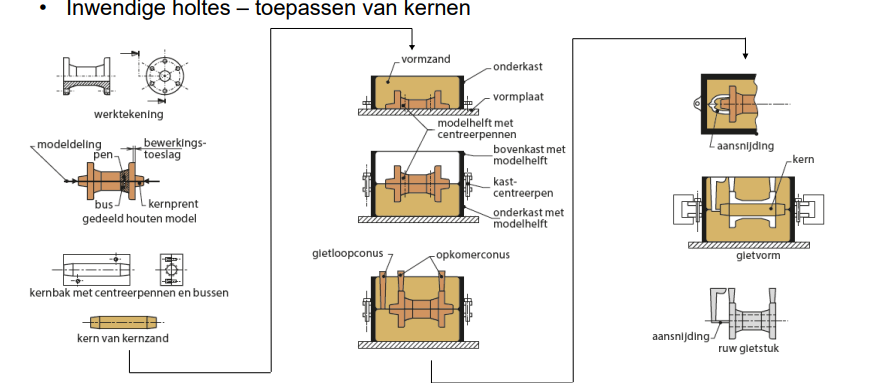
\includegraphics[width=1\textwidth]{assets/Kernen_gieten.png}
    \caption{Kernen bij gieten}
    \label{fig:Kernen_gieten.png}
\end{figure}
\FloatBarrier

Je neemt de buitenkant van het product eerst en je plaatst dan je kern in het gietstuk.
Dit is wel wat werk want je moet bij elke keer dat je giet dit herhalen. Vandaag de dag
kunnen veel van deze taken door robots worden gedaan.

\subsection{Automatisch maken van zandvormen}
Je gaat een profiel maken voor je zandvorm.
Deze worden door een machine geperst en dan afgevoerd. Het grote werk van
zandvormen maken wordt zo geautomatiseerd.

\begin{figure}[htbp]
    \centering
    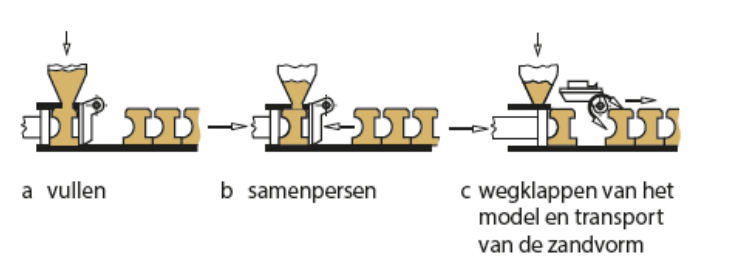
\includegraphics[width=0.8\textwidth]{assets/Autozandvormen.png}
    \caption{Automatisch maken van zandvormen: gebruik van geautomatiseerde systemen om zandvormen te produceren voor metaalgieten}
    \label{fig:Autozandvormen.png}
\end{figure}

Je zand kan kleigebonden, chemisch gebonden of schaalvormend zijn.

\begin{conceptbox}[Soorten zandbinding]
    \begin{itemize}
        \item \textbf{Kleigebonden zand}: Traditioneel zandmengsel met klei en water. Goedkoop en eenvoudig, maar minder sterk en duurzaam.
        \item \textbf{Chemisch gebonden zand}: Zand gemengd met chemische bindmiddelen die uitharden bij kamertemperatuur of door verhitting. Biedt betere sterkte en precisie.
        \item \textbf{Schaalvormend zand}: Fijn zandmengsel dat een harde schaal vormt rond een patroon. Geschikt voor complexe vormen en biedt hoge precisie.
    \end{itemize}
\end{conceptbox}

\subsection{Afwerken van zandgietstukken}
Na het gietproces moet je de opkomers en de gietloop afbreken en het oppervlak nabewerken.
Dit kan gedaan worden door brandsnijden, slijpen, schuren of polijsten.

De oppervlaktekwaliteit van zandgieten is slecht ($R_a$ rond \SI{6}{\micro m} tot \SI{12}{\micro m}),
dus je zult nog moeten nabewerken.
Schaalvormen geven een beter oppervlak ($R_a$ rond \SI{3}{\micro m} tot \SI{6}{\micro m}).

\begin{examenbox}
    Zorg dat je de kenmerken van zandgieten kent:
    \begin{itemize}
        \item goedkoop
        \item grote maten mogelijk
        \item slechte oppervlaktekwaliteit
        \item lage precisie
        \item geschikt van enkelstuks tot grote series (met geautomatiseerde vormerij)
    \end{itemize}
\end{examenbox}

\section{Verloren-modelmethode}
\subsection{Verloren wasmodel}

\begin{wrapfigure}{r}{0.3\textwidth}
    \centering
    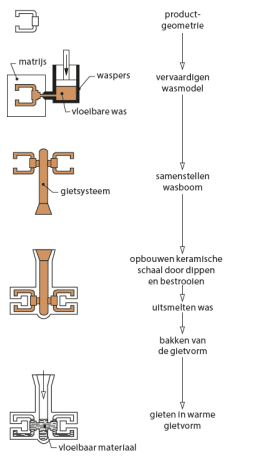
\includegraphics[width=0.3\textwidth]{assets/verlorenwasgieten.png}
    \caption{Verloren wasmodel proces: maken van keramische vormen door dompelen van wasmodellen voor metaalgieten}
    \label{fig:Verlorenwasmodel.png}
\end{wrapfigure}
\FloatBarrier

Je kunt modellen maken uit was.

Dat wasmodel dompel je (herhaaldelijk) in een keramische slurry.
De uitgeharde slurry vormt een harde schaal rond het wasmodel.
Zodra die schaal de gewenste dikte heeft, smelt je de was eruit.
Je hebt nu een holle keramische vorm.
Je kunt nu metaal gieten in deze keramische vorm en dan de keramische vorm breken om je product eruit te halen.

In tegenstelling tot zandgieten is de oppervlaktekwaliteit en nauwkeurigheid veel beter.
Dit komt omdat de keramische schaal veel fijner is dan zand.
Je kunt ook complexere vormen maken omdat je geen vormkasten nodig hebt.
Grote stukken zijn wel moeilijk: de keramische schaal moet dan lang drogen en wordt lastig te maken en te dragen.


\subsection{Verloren schuim-model}
Je maakt een model uit schuim zoals piepschuim.
Je plaatst dit in een bak of vormkast en je verbrandt dan het schuim.
Je giet dan metaal in de holte die het schuim heeft achtergelaten.
Het is heel gelijkaardig aan verloren wasmodel.
Net zoals bij het verloren wasmodel zijn de oppervlaktekwaliteit en de nauwkeurigheid beter dan bij zandgieten.
Je kunt ook complexere vormen maken omdat je geen vormkasten nodig hebt.
Grote stukken blijven wel lastig.

\begin{table}[htbp]
    \centering
    \caption{Vergelijking van verschillende gietprocessen}
    \label{tab:gietprocessen}
    \small
    \renewcommand{\arraystretch}{1.1}
    \setlength{\tabcolsep}{4pt}
    \begin{tabularx}{\textwidth}{@{} >{\bfseries}l | X | X | X | X @{}}
        \toprule
        \textnormal{\textbf{Eigenschap}} & \textbf{Zand} & \textbf{Was}     & \textbf{Schuim}  & \textbf{Matrijs}  \\
        \midrule
        Ruwheid $R_a$ (\si{\micro m})    & Ruw (10--25)  & Zeer goed (1--3) & Goed (2--10)     & Uitstekend (1--2) \\
        Maattolerantie                   & $\pm$ 1--2 mm & $\pm$ 0,1 mm     & $\pm$ 0,3 mm     & $\pm$ 0,1 mm      \\
        Vormvrijheid                     & Hoog          & Zeer hoog        & Zeer hoog        & Beperkt           \\
        Min. wanddikte                   & 3--5 mm       & 0,5--1 mm        & 2--3 mm          & 1--2 mm           \\
        Seriegrootte                     & 1 tot groot   & Klein tot middel & Middel tot groot & Massa             \\
        Matrijskosten                    & Laag          & Gemiddeld        & Laag             & Zeer hoog         \\
        Stukprijs                        & Hoog          & Hoog             & Gemiddeld        & Laag              \\
        Materialen                       & Alle metalen  & Alle metalen     & Alle metalen     & Non-ferro         \\
        \bottomrule
    \end{tabularx}
\end{table}

\section{Gieten in permanente vormen}
Permanente vormen kun je blijven hergebruiken.
Ze werken uitstekend voor kunststoffen, maar voor metalen geldt een harde grens: het gegoten metaal
mag geen hógere smelttemperatuur hebben dan de vorm zelf aankan. Daarom beperkt dit zich in de praktijk
tot non-ferrometalen (aluminium, zink, magnesium, koper).

Je hebt verschillende technieken:
\begin{itemize}
    \item \textbf{Coquillegieten}: Je giet gesmolten metaal in een metalen matrijs die gekoeld wordt. De druk wordt geleverd door
          zwaartekracht.
          Gebruikt voor simpele stukken in grote series.
    \item \textbf{Lagedrukgieten}: Je perst gesmolten metaal met lage druk (\SI{30}{kPa} tot \SI{100}{kPa})
          van onderaf in een metalen matrijs. Rustige vulling, dus weinig insluitingen.
          Gebruikt voor aluminium velgen.
    \item \textbf{Spuitgieten (die casting)}: Je spuit gesmolten metaal onder hoge druk in een metalen matrijs.
          Gebruikt voor complexe stukken in grote series, door de hoge snelheid en precisie.
          Denk aan een wafelijzer waar je vloeibaar metaal in spuit.
\end{itemize}

De verschillen tussen deze technieken zitten vooral in de druk en snelheid van het gieten.
Hoe hoger de druk en snelheid, hoe beter de oppervlaktekwaliteit en nauwkeurigheid.
Deze hangt ook af van de vorm natuurlijk.

Technieken zoals kernen en opkomers komen hier ook terug.
\begin{examenbox}
    Zorg dat je de kenmerken van permanent gieten kent:
    \begin{itemize}
        \item duur in opstart
        \item hoge precisie
        \item goede oppervlaktekwaliteit
        \item geschikt voor grote series
        \item Betere kwaliteit bij hogere druk/snelheid
    \end{itemize}
\end{examenbox}

\subsection{Verschillende soorten spuitgieten}
Je hebt verschillende soorten spuitgieten:
\begin{itemize}
    \item \textbf{Cold-chamber spuitgieten}: De vulkamer en de zuiger staan \emph{buiten} het smeltbad.
          Je schept het metaal er per schot in en perst het dan in de matrijs.
          Gebruikt voor metalen met een hogere smelttemperatuur: aluminium, magnesium en koperlegeringen.
          Drukken van \SI{15}{MPa} tot \SI{70}{MPa}; matrijzen gaan 50.000 tot 250.000 stukken mee.
    \item \textbf{Hot-chamber spuitgieten}: De vulkamer en de zuiger staan \emph{in} het smeltbad,
          zodat het metaal er vanzelf instroomt. Sneller, maar de zuiger staat permanent in vloeibaar metaal.
          Alleen bruikbaar voor laagsmeltende metalen die de zuiger niet aantasten: zink, tin en lood.
          Drukken van \SI{3}{MPa} tot \SI{30}{MPa}; matrijzen gaan tot ongeveer 1.000.000 stukken mee.
\end{itemize}

Het verschil zit dus niet in de temperatuur van de kamer op zich, maar in de vraag of de vulkamer
mee in het smeltbad staat of niet. Dat bepaalt meteen welke metalen je kunt verwerken.

\textit{Tip: bekijk zeker de video's van deze processen terug op Toledo. Die leggen het beter uit dan ik hier kan.}

\section{Keuze van gietmethode}
Je kiest een gietmethode op basis van:
\begin{itemize}
    \item \textbf{Wanddikte}: dunne wanden vereisen permanente vormen (het metaal moet er snel in).
    \item \textbf{Productaantal}: grote series verantwoorden de dure permanente vorm.
    \item \textbf{Oppervlaktekwaliteit}: hoge kwaliteit vraagt permanente vormen of verloren was.
    \item \textbf{Nauwkeurigheid}: hoge nauwkeurigheid vraagt permanente vormen of verloren was.
    \item \textbf{Complexiteit van de vorm}: erg complexe vormen vragen verloren modellen.
    \item \textbf{Afmetingen}: heel grote stukken kunnen enkel met zandgieten.
\end{itemize}

\begin{figure}[htbp]
    \centering
    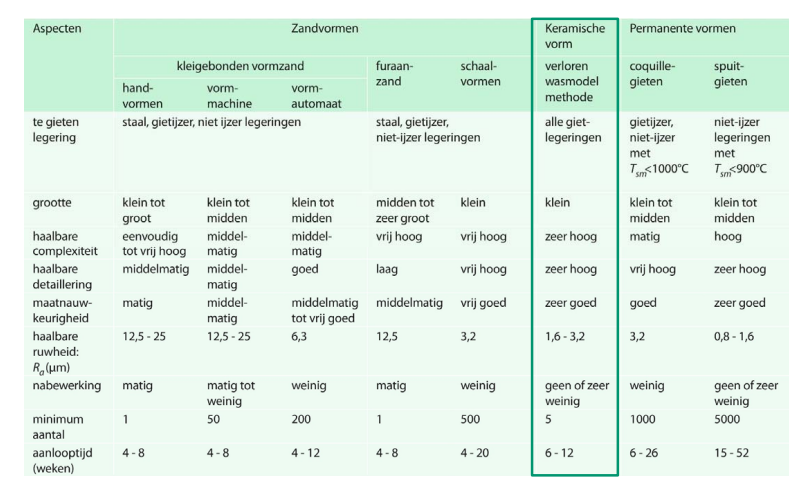
\includegraphics[width=1\textwidth]{assets/Kostenverschillendetechniekengieten.png}
    \caption{Kostenverschillen tussen verschillende giettechnieken: vergelijking van initiële kosten en stukkosten voor zandgieten,
        verloren wasgieten, verloren schuimgieten en permanent gieten}
    \label{fig:Kostenverschillendetechniekengieten.png}
\end{figure}

Je moet dus je keuze maken afhankelijk van de toepassing en de prijs.

\subsection{Ontwerp aanpassen aan gieten}
Het nadeel bij gieten is dat je ontwerp moet aangepast worden aan het gieten.
Grote volumes zijn riskant door \belangrijk{slink} en \belangrijk{krimp}.
Je moet ook zorgen voor \belangrijk{lossing} zodat je het product uit de vorm kunt halen.
Je moet ook zorgen voor \belangrijk{opkomers} zodat je slink kunt vermijden.
Je moet ook zorgen voor \belangrijk{vormkasten} zodat je complexe vormen kunt maken.

\begin{figure}[htbp]
    \centering
    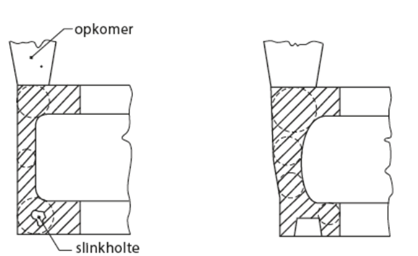
\includegraphics[width=0.4\textwidth]{assets/verschildesigngieten.png}
    \caption{Design aanpassen aan gieten}
    \label{fig:Ontwerpoverwegingenbijgieten.png}
\end{figure}
\FloatBarrier

In de figuur zijn grote volumes vermeden om slinkholtes te voorkomen.
Scherpe hoeken zijn afgerond zodat je het stuk makkelijker uit de mal kunt halen.

\begin{warningbox}[EXAMEN CHECKLIST: OERVORMEN]
    \begin{itemize}
        \item \textbf{Stollen}: Begrijp het verschil tussen \textbf{Slink} (stollen) en \textbf{Krimp} (afkoelen).
        \item \textbf{Opkomers}: Leg uit waarom opkomers nodig zijn (reservoirs tegen slink) en ken directionele stolling.
        \item \textbf{Zandgieten}: Ken de voordelen (grootte, prijs) en nadelen (precisie, oppervlak).
        \item \textbf{Verloren-model}: Begrijp de was- en schuimmethode voor complexe vormen.
        \item \textbf{Permanente vormen}: Ken spuitgieten (hot vs.\ cold chamber) en waarom je hier beperkt bent tot non-ferrometalen.
    \end{itemize}
\end{warningbox}

\chapter{Productie machines en automatisering}

\begin{conceptbox}[Productietijd]
    De totale productietijd per stuk wordt bepaald door:
    \[ T_{tot} = T_h + T_n \]
    \begin{itemize}
        \item \textbf{Hoofdtijd ($T_h$)}: De tijd waarin daadwerkelijk materiaal wordt weggenomen.
        \item \textbf{Neventijd ($T_n$)}: De tijd voor opspannen, gereedschapswissels, instellen en programmeren.
              Automatisering richt zich vooral op het minimaliseren van $T_n$.
    \end{itemize}
\end{conceptbox}

We hebben nu een groot aantal productieprocessen gezien, maar hoe werken de machines die deze
processen uitvoeren?

\section{Inleiding}
Aan productiemachines worden, afhankelijk van het proces, een aantal eisen gesteld.

\begin{figure}[htbp]
    \centering
    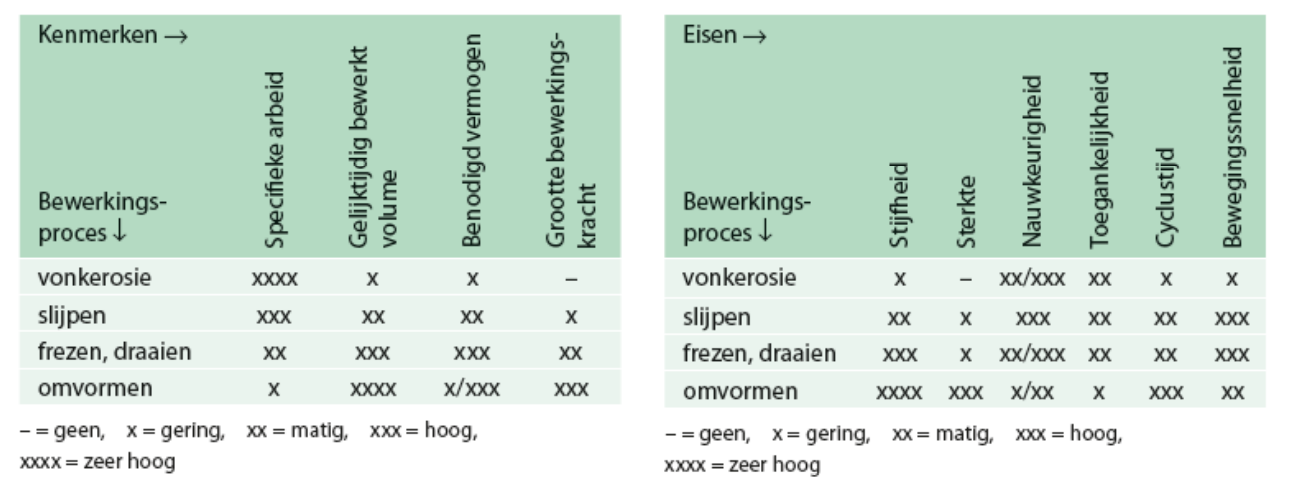
\includegraphics[width=1\textwidth]{assets/kenmerkeneneisenmachines.png}
    \caption{De kenmerken en eisen van productiemachines: overzicht van de belangrijkste eigenschappen en vereisten voor machines die worden gebruikt in productieprocessen}
    \label{fig:kenmerkeneneisenmachines.png}
\end{figure}
\FloatBarrier

Welke energie heb je nodig, en in welke vorm moet die omgezet worden (kinetisch, warmte, \ldots)?
Hoe moet de machine bewegen?
Een draaimachine moet het werkstuk laten roteren; een freesmachine moet de frees laten roteren
én de tafel lineair verplaatsen in drie richtingen.
Al die eisen samen bepalen de snelheden waarmee de machine moet kunnen werken.

Hoe worden werkstukken geklemd?
Ze mogen namelijk niet bewegen tijdens het bewerken of alleen bewegen langs gewenste vrijheidsrichtingen.

De stijfheid van de machine is ook belangrijk voor je nauwkeurigheid.

Je hebt dan manuele en automatische machines.

\section{Waarom automatiseren?}
Automatiseren verhoogt bij grote productieaantallen de productiviteit, vooral door de \textbf{neventijd}
$T_n$ te drukken: in- en uitladen, instellen, gereedschapswissels, metingen en correcties.
De hoofdtijd $T_h$ ligt immers grotendeels vast door het proces zelf (snijsnelheid, voeding).
Bij enkelstuks weegt de programmeer- en insteltijd juist zwaar door, en daar loont automatiseren minder.

\subsection{Starre automatiseringen}
\vspace{0.2cm}
\begin{figure}[htbp]
    \centering
    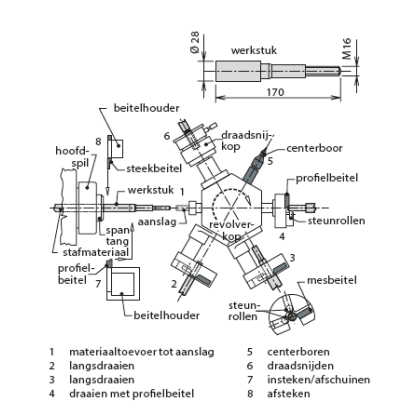
\includegraphics[width=0.55\textwidth]{assets/image85.png}
    \caption{Starre automatisering: gebruik van vaste, niet-aanpasbare systemen voor productieprocessen}
    \label{fig:Starreautomatisering.png}
\end{figure}
\FloatBarrier

Bij een revolverdraaibank automatiseer je de machine \emph{mechanisch}, met nokken en aanslagen.
Je hebt verschillende beitelposities in een revolverkop die automatisch wisselen en elk een operatie uitvoeren.
Zo voer je meerdere bewerkingen uit zonder tussenkomst van een operator.
Eenmaal ingesteld gaat dit razendsnel, maar het \emph{instellen} zelf is tijdrovend, en voor elk nieuw
product moet je alles opnieuw mechanisch afregelen. Vandaar de naam \emph{starre} automatisering.

\subsection{NC-gestuurde machines}

Vandaag wordt starre automatisering nog nauwelijks gebruikt: NC-gestuurde machines hebben het overgenomen.
Die werken met \textbf{G-code}, van 3D-printers tot CNC-freesmachines.
De meeste G-code is gelijkaardig en geeft controle over de voedingssnelheid, het gereedschap,
het spiltoerental, de koelvloeistof, de bewegingen enzovoort.
Het nadeel is dat G-code op zich geen \emph{overzicht} geeft van de bewerkingen die je uitvoert:
je ziet enkel een lange lijst coördinaten.
Daarom hebben NC-machines vaak een interface waarin je bewerkingen visueel kunt opbouwen.
\textit{Denk aan de visuele quick-code van de labo's.}
Met G-code kun je bovendien gereedschapswissels programmeren, werkstukken verwisselen
en bewerkingen met meerdere spillen uitvoeren.


Voorbeeld van G-code (frezen van een vierkant van 50x50 mm):
\begin{tcolorbox}[colback=black!5,colframe=black!50,title=G-code Voorbeeld]
    \begin{verbatim}
G21          ; Gebruik metrische eenheden (mm)
G90          ; Absolute positionering
T1 M6        ; Gereedschapswissel naar gereedschap 1
M3 S2000     ; Start spindel (2000 RPM)
G0 X0 Y0 Z5  ; Snelverplaatsing naar startpunt boven werkstuk
G1 Z-2 F100  ; Lineaire verplaatsing naar diepte -2mm (voeding 100)
G1 X50 F500  ; Frees naar X=50
G1 Y50       ; Frees naar Y=50
G1 X0        ; Frees naar X=0
G1 Y0        ; Frees naar Y=0
G0 Z5        ; Trek gereedschap terug naar veilige hoogte
M5           ; Stop spindel
M30          ; Einde programma
\end{verbatim}
\end{tcolorbox}


\subsection{Toepassingsgebied van productiesystemen (K-grafiek)}
De keuze voor een productiesysteem wordt bepaald door de balans tussen de \textbf{seriegrootte} en de \textbf{moeilijkheidsgraad}
(of het afkeurrisico) van het product.
In de onderstaande grafiek (vaak ook de K-grafiek genoemd in deze context) zien we hoe verschillende technologieën
zich tot elkaar verhouden.

\begin{itemize}
    \item \textbf{Handbediende machines}: Ideaal voor kleine series met een lage moeilijkheidsgraad.
    \item \textbf{Mechanisch bestuurde machines (starre automatisering)}: Geschikt voor zeer grote series met een beperkte complexiteit.
    \item \textbf{NC-machines}: Deze vullen het middengebied in en zijn door hun flexibiliteit uiterst geschikt voor complexe producten.
\end{itemize}

De evolutie in de technologie (weergegeven door de verschuiving van de gestreepte naar de doorgetrokken lijnen)
laat zien dat NC-machines een steeds groter gebied bestrijken.
Ze worden rendabeler bij zowel kleinere series (door kortere insteltijden) als grotere series (door hogere productiviteit),
en kunnen steeds complexere taken aan.

\begin{figure}[htbp]
    \centering
    \begin{tikzpicture}[>=Stealth, font=\sffamily\small, scale=1.1]
        % Assen tekenen
        \draw[thick, ->] (0,0) -- (0,7) node[midway, left=25pt, rotate=90, anchor=south] {seriegrootte};
        \draw[thick, ->] (0,0) -- (8,0) node[anchor=north west] {moeilijkheidsgraad, afkeurrisico};

        % De horizontale scheidingslijn aan de linkerkant
        \draw (0, 2) -- (2, 2);

        % De gestreepte lijnen (starten vanaf het midden van de horizontale lijn) - Oude situatie
        \draw[dashed, gray] (1, 2) -- (4, 6.5);
        \draw[dashed, gray] (1, 2) -- (2.5, 0);

        % De doorgetrokken lijnen (starten vanaf het uiteinde van de horizontale lijn) - Nieuwe situatie
        \draw[thick] (2, 2) -- (5, 6.5);
        \draw[thick] (2, 2) -- (3.5, 0);

        % Tekst labels toevoegen
        % Linksboven
        \node[align=left, anchor=west] at (0.2, 5) {mechanisch\\bestuurde\\machines};
        % Rechtsboven
        \node[align=left, anchor=west] at (4.5, 6) {meerspillige NC-machines};
        % Linksonder
        \node[align=left, anchor=west] at (0.2, 0.8) {hand-\\bediende\\machines};
        % Midden rechts
        \node[align=left, anchor=west] at (2.5, 2.2) {NC-draaimachines en\\bewerkingscentra};
        % Rechtsonder
        \node[align=left, anchor=west] at (4.5, 0.5) {5-assige NC-freesmachines};
        % Legenda/Indicatie verschuiving (Arrows reversed: now pointing towards the boundaries to show expansion)
        \draw[<-, green!60!black, thick] (1.2, 3) -- (1.8, 3) node[midway, above, font=\tiny] {Evolutie};
        \draw[<-, green!60!black, thick] (1.8, 1) -- (2.4, 1) node[midway, below, font=\tiny] {Evolutie};
    \end{tikzpicture}
    \caption{K-grafiek: Toepassingsgebied van diverse productiesystemen in functie van seriegrootte en moeilijkheidsgraad. De verschuiving van de grenzen toont de groeiende inzetbaarheid van NC-technologie.}\label{fig:k_grafiek_user}
\end{figure}
\FloatBarrier

\subsection{CAM}

\begin{wrapfigure}{r}{0.35\textwidth}
    \centering
    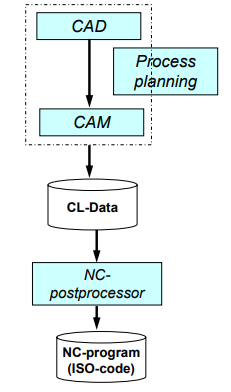
\includegraphics[width=0.35\textwidth]{assets/WorkflowCADCAM.png}
    \caption{Workflow van CAD naar CAM: proces van het ontwerpen van modellen in
        CAD-software en het genereren van bewerkingsprogramma's in CAM-software voor productie}
    \label{fig:WorkflowCADCAM.png}
\end{wrapfigure}
\FloatBarrier

\textbf{CAD} (Computer Aided Design) is het ontwerpen van modellen op de computer.

\textbf{CAM} (Computer Aided Manufacturing) is het omzetten van deze modellen naar bewerkingsprogramma's.

Vandaag de dag werken deze dingen hand in hand met de computer.
Je ontwerpt een model in CAD en importeert dat model daarna in CAM-software.
In deze CAM-software kun je dan bewerkingen definiëren zoals frezen, boren, zagen, enz.
De CAM-software genereert dan CL-data, dit is coördinaatcode (geen G-code),
daarna wordt er voor de specifieke machine G-code gegenereerd.
In de moderne industrie wordt dit allemaal toegepast.
Je maakt je CAD, je importeert in CAM, je genereert CL-code en je stuurt dit naar de machine via een netwerk.
NC-machines op het netwerk zetten kan ook helpen voor monitoring en onderhoud. Je kunt stappen via de computer volgen.

\vspace{1cm}
\begin{warningbox}[EXAMEN CHECKLIST: MACHINES \& AUTOMATISERING]
    \begin{itemize}
        \item \textbf{Tijden}: Ken het verschil tussen hoofdtijd en neventijd en de invloed van seriegrootte op de totale kosten.
        \item \textbf{Automatisering}: Onderscheid starre (mechanische) en flexibele (NC/CNC) automatisering.
        \item \textbf{G-code}: Begrijp de structuur van een G-programma (G0, G1, M-functies).
        \item \textbf{K-grafiek}: Leg uit hoe de inzetbaarheid van NC-machines groeit door lagere instelkosten en hogere flexibiliteit.
        \item \textbf{CAD/CAM}: Begrijp de workflow van digitaal ontwerp naar machine-instructies via CL-data en post-processing.
    \end{itemize}
\end{warningbox}

\chapter{Productie werkvoorbereiding}
\section{Inleiding}
Werkvoorbereiding is het proces waarbij je alle stappen plant en organiseert die nodig zijn om een product te maken.

De centrale vraag bij werkvoorbereiding is: \textbf{Hoe gaan we dit product maken met de beschikbare middelen?}

Niet elk bedrijf heeft alle mogelijke productieprocessen in huis.
Je moet dus keuzes maken op basis van wat er beschikbaar is (machinepark, gereedschappen) of beslissen wat eventueel uitbesteed
moet worden.

Het totale voortbrengingsproces doorloopt doorgaans de volgende stadia:
\begin{enumerate}
    \item \textbf{Materiaalbereiding}: De winning en basisverwerking van grondstoffen tot halffabricaten.
    \item \textbf{Primaire vormgeving (Oervormen)}: Het creëren van een eerste ruwe vorm uit vormloos materiaal.
          Een typisch voorbeeld is gieten, wat vaak rendabel is bij grotere series.
    \item \textbf{Secundaire vormgeving (Bewerken)}: De verdere afwerking van de ruwe vorm naar een nauwkeurig product. Dit omvat technieken zoals verspanen (frezen, draaien), lassen of buigen.
    \item \textbf{Materiaalbehandeling}: Het aanpassen van de intrinsieke materiaaleigenschappen, bijvoorbeeld de hardheid verhogen door een warmtebehandeling.
    \item \textbf{Oppervlaktebehandeling}: Het wijzigen van de eigenschappen van het oppervlak, bijvoorbeeld voor corrosiebescherming of esthetiek (coaten, anodiseren, lakken).
    \item \textbf{Montage of assemblage}: Het samenvoegen van de verschillende geproduceerde onderdelen tot één werkend eindproduct.
\end{enumerate}

\textbf{Macrowerkmethode}: je kijkt op hoog niveau hoe je het product gaat maken.
Welke machines en processen ga je gebruiken, in welke volgorde, en welke bewerkingen en afnames zijn nodig?

\textbf{Microwerkmethode}: Hier ga je duiken in de details zoals wat is de voeding die ik moet gebruiken.
Welke snijsnelheid, welke gereedschappen, welke koelvloeistof, enz.

\section{Het bewerkingsplan. De macrowerkmethode}
Het bewerkingsplan is relevant voor de macrowerkmethode.
Hier ga je kijken naar de verschillende processen die je kunt gebruiken om je product te maken.
Je bewerkingsplan hangt af van heel wat factoren:
\begin{itemize}
    \item \textbf{Seriegrootte en totaalserie}: Hoeveel producten ga je maken. Bij grote series kun je investeren in
          duurdere machines en processen.
    \item \textbf{Werkstukmateriaal}: Je hebt zacht maar ook harde materialen. Soms limiteert dit je keuze van proces.
    \item \textbf{Toleranties}: Hoe nauwkeurig moet het product zijn.
    \item \textbf{Afmetingen en vorm}: De geometrie van het product kan bepaalde processen uitsluiten of sommige processen vereisen.
    \item \textbf{Beschikbare machines en middelen}: Je moet kijken wat er beschikbaar is in de fabriek en het personeel dat je hebt.
    \item \textbf{Levertijd}: Hoe snel moet het product klaar zijn. Sommige processen zijn sneller dan andere.
\end{itemize}

Je moet duidelijk weten wat mogelijk is en wat de beperkingen zijn.
De kosten van deze processen moeten ook in rekening worden gebracht.
Bij het opstellen van een bewerkingsplan is er vaak niet één enkel correct antwoord; verschillende keuzes kunnen verdedigbaar zijn,
zolang ze goed gemotiveerd worden op basis van factoren zoals de vereiste nauwkeurigheid, de kostprijs,
de productiesnelheid en de seriegrootte.

\begin{examenbox}
    Motiveer je keuzes voor een specifiek proces altijd aan de hand van technische en economische criteria.
\end{examenbox}

\subsection{Positionering}

\begin{conceptbox}[3-2-1 Methode]
    Om een werkstuk eenduidig vast te leggen in de ruimte (alle 6 vrijheidsgraden beperken), gebruiken we de 3-2-1 regel:
    \begin{itemize}
        \item \textbf{3 punten} bepalen het hoofdvlak (beperkt 3 vrijheidsgraden).
        \item \textbf{2 punten} bepalen de oriëntatie (beperkt 2 vrijheidsgraden).
        \item \textbf{1 punt} bepaalt de positie (beperkt de laatste vrijheidsgraad).
    \end{itemize}
\end{conceptbox}

Bij het positioneren wordt het werkstuk nauwkeurig in de machine geplaatst ten opzichte van een gekozen nulpunt of referentievlak.
Het doel is om het werkstuk eenduidig vast te leggen in de ruimte,
zodat de machine exact weet waar de bewerkingen moeten plaatsvinden.
Hiervoor moet men vaak eerst een referentievlak bepalen door het werkstuk op te meten.

\begin{figure}[htbp]
    \centering
    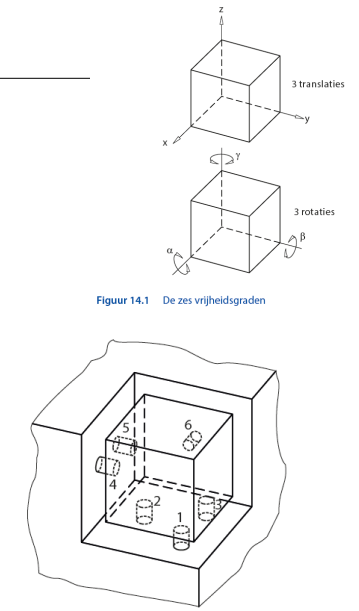
\includegraphics[width=0.3\textwidth]{assets/positioneren.png}
    \caption{Positioneren van het werkstuk volgens het 3-2-1 principe: bepalen van de juiste oriëntatie en referentiepunten.}
    \label{fig:positionerenwerkstuk}
\end{figure}
\FloatBarrier

Een fundamenteel principe hierbij is de \textbf{3-2-1 methode},
die wordt gebruikt om de vrijheidsgraden van het werkstuk te minimaliseren en het eenduidig te positioneren:
\begin{itemize}
    \item \textbf{3 punten} bepalen het primaire vlak (meestal het grootste steunvlak).
    \item \textbf{2 punten} bepalen de oriëntatie ten opzichte van een tweede, loodrecht vlak.
    \item \textbf{1 punt} bepaalt de definitieve positie ten opzichte van het derde vlak.
\end{itemize}
Op deze manier ligt de positie van het werkstuk volledig vast zonder dat het systeem overbepaald is.

\subsection{Klemmen}

Nadat het werkstuk correct is gepositioneerd, moet het stevig worden vastgezet (opgespannen).
Het doel van klemmen is om alle resterende vrijheidsgraden weg te nemen en te garanderen dat het werkstuk niet verschuift of
trilt onder invloed van de proceskrachten (zoals de snijkrachten van de frees of beitel).
De klemming gebeurt meestal door middel van wrijvingskrachten of directe mechanische klemkracht.

Er zijn verschillende methoden en hulpmiddelen beschikbaar voor het opspannen:

\begin{itemize}
    \item \textbf{Bankschroef}: De meest gebruikte methode voor prismatische werkstukken.
    \item \textbf{T-bouten en klemplaten}: Hiermee kan het werkstuk direct op de machinetafel worden gemonteerd.
    \item \textbf{Magneetklemmen}: Vooral geschikt voor vlakke, ferromagnetische materialen (vaak bij slijpen).
    \item \textbf{Vacuümklemmen}: Ideaal voor het opspannen van dunne platen of niet-magnetische materialen.
\end{itemize}

\begin{figure}[htbp]
    \centering
    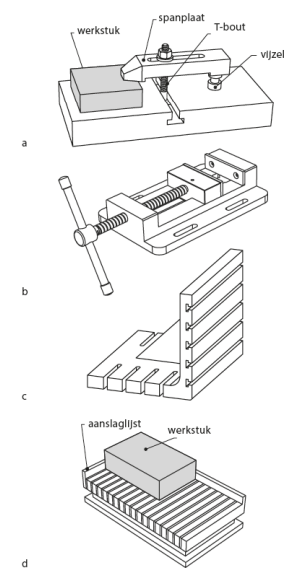
\includegraphics[width=0.3\textwidth]{assets/image82.png}
    \caption{Klemmen van het werkstuk: diverse methoden om het werkstuk stabiel te fixeren tijdens de bewerking.}
    \label{fig:klemmenwerkstuk}
\end{figure}

\subsection{Ondersteuning}

Naast positionering en klemmen is ondersteuning cruciaal, zeker bij complexe of minder stijve werkstukken.
Ondersteuning dient niet enkel om het eigen gewicht van het stuk te dragen, maar vooral om vervorming door de grote snijkrachten
tegen te gaan.

Zonder de juiste ondersteuning kan het werkstuk gaan doorbuigen of kunnen er trillingen (\textit{chatter}) ontstaan.
Dit leidt tot een slechte oppervlaktekwaliteit en afwijkingen in de maatvoering.
In de figuur hieronder is te zien hoe ondersteuning helpt om deze buiging te voorkomen.

\begin{figure}[htbp]
    \centering
    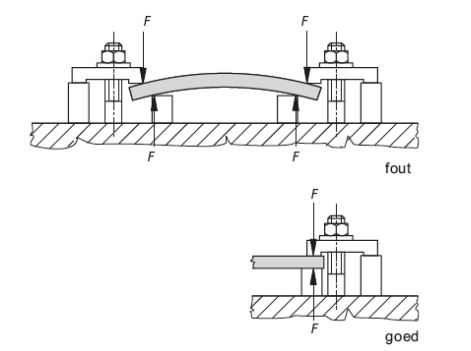
\includegraphics[width=0.4\textwidth]{assets/voorkomenbuiging.png}
    \caption{Ondersteuning van het werkstuk: het gebruik van steunpunten om doorbuiging en
        trillingen tijdens de bewerking te minimaliseren.}
    \label{fig:voorkomenbuiging}
\end{figure}

\subsection{Universeel en product specifiek opspansysteem}

Een belangrijke keuze in het bewerkingsplan is het type opspansysteem.
Afhankelijk van de seriegrootte en de diversiteit van de producten, kies je tussen een universeel of een productspecifiek systeem.

\begin{itemize}

    \item \textbf{Productspecifiek opspansysteem}: Bij grote series is het rendabel om een opspanning op maat te maken (een mal).
          Het ontwerpen en maken kost tijd en geld, maar het wisselen van werkstukken gaat daarna zeer snel en nauwkeurig.

    \item \textbf{Universeel opspansysteem}: Bij kleine series of enkelstuks is flexibiliteit belangrijker.
          Universele systemen (zoals modulaire opspantafels) werken als een bouwdoos met gatenpatronen, klemmen en steunen. Hiermee kun je snel schakelen tussen verschillende producten zonder hoge investeringskosten per product.

\end{itemize}


\begin{figure}[htbp]
    \centering
    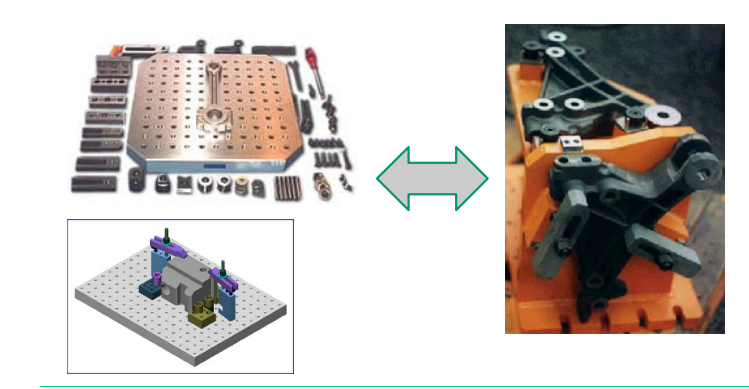
\includegraphics[width=0.6\textwidth]{assets/universeeltegenspecifiek.png}
    \caption{Universeel klemmen versus productspecifiek klemmen: flexibele modulaire systemen versus op maat gemaakte mallen.}
    \label{fig:universeeltegenspecifiek}
\end{figure}

\subsection{Nauwkeurigheid en ruwheid}
Het bewerkingsplan wordt sterk bepaald door de vereiste toleranties en oppervlaktekwaliteit. Niet elk proces kan elke nauwkeurigheid halen.

\begin{figure}[htbp]
    \centering
    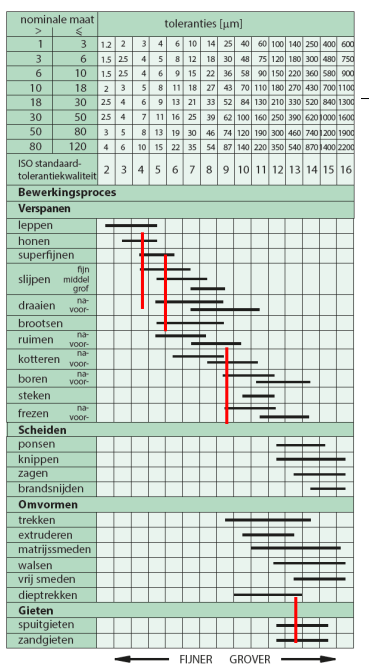
\includegraphics[width=0.45\textwidth]{assets/tolerantie.png}
    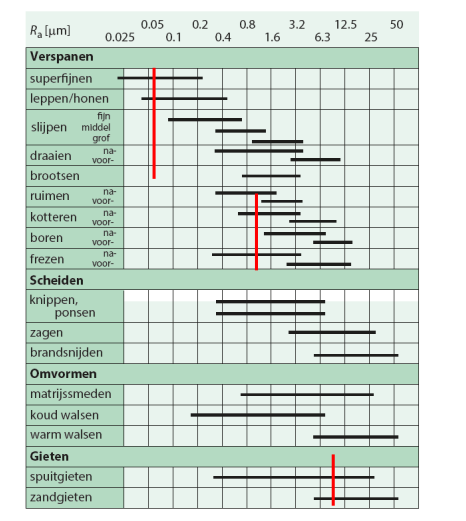
\includegraphics[width=0.45\textwidth]{assets/Ruwheid.png}
    \caption{Toleranties en ruwheid van verschillende bewerkingsprocessen: overzicht van haalbare maattoleranties en oppervlaktekwaliteiten.}
    \label{fig:tolerantieRuwheid}
\end{figure}
\FloatBarrier

\section{Microvoorbereiden en bewerkingsstappen}
Bij de microwerkmethode kijk je naar de specifieke stappen binnen één bewerking.
Hierbij maak je onderscheid tussen ruwen en afwerken.

\begin{conceptbox}[Ruwen (roughing) en afwerken (finishing)]
    \textbf{Ruwen (roughing):} Het doel is zo snel mogelijk materiaal verwijderen (hoge \textit{material removal rate}).
    Je gebruikt grote snededieptes en voedingen. Oppervlaktekwaliteit en maattolerantie zijn hier nog van minder belang.
    \newline
    \textbf{Afwerken (finishing):} Na het ruwen volgt de nabewerking om de definitieve maatvoering en
    oppervlaktekwaliteit te bereiken. Hier werk je met kleine afnames en fijne voedingen.
\end{conceptbox}

Vaak zijn er meerdere stappen nodig (bijvoorbeeld grof ruwen, voorafwerken, afwerken) om de gewenste
nauwkeurigheid te halen, zeker als er veel materiaal weggenomen moet worden waardoor interne spanningen vrijkomen.

\begin{figure}[htbp]
    \centering
    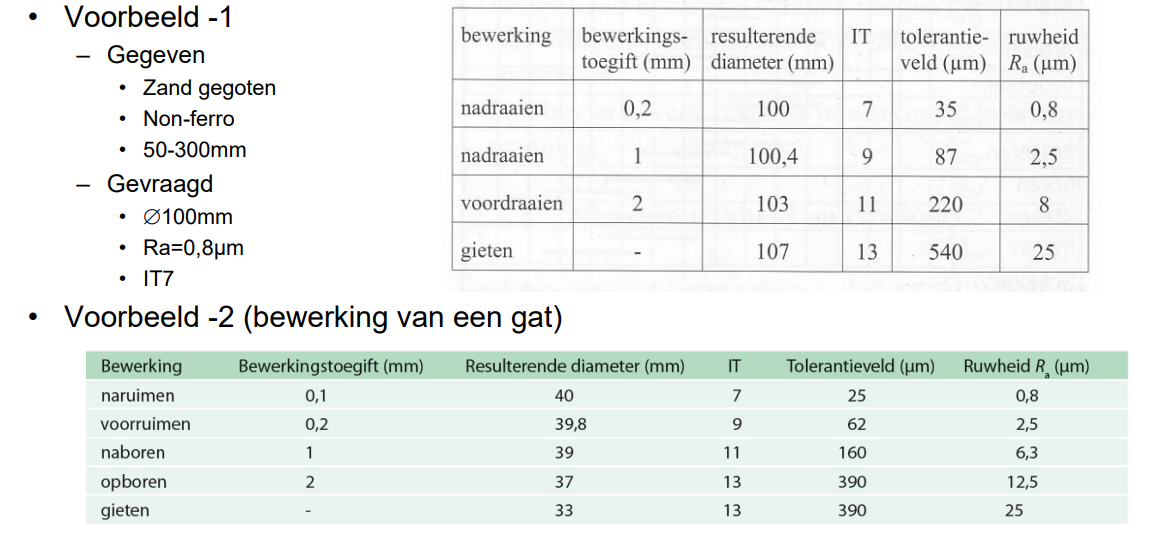
\includegraphics[width=1\textwidth]{assets/image83.png}
    \caption{Bewerkingstoegift: eerst ruwen met grote afnames, daarna afwerken met kleine afnames voor het eindresultaat.}
    \label{fig:image83}
\end{figure}

\subsection{Computerondersteunde werkvoorbereiding (CAPP)}
Computer Aided Process Planning (CAPP) automatiseert het maken van werkvoorbereidingen. We onderscheiden twee hoofdmethoden:

\begin{itemize}
    \item \textbf{Variant methode (Retrieval type)}: Het systeem zoekt in een database naar een bestaand bewerkingsplan van een vergelijkbaar product (een "variant") en past dit aan voor het nieuwe product. Dit is gebaseerd op Groepentechnologie (GT).
    \item \textbf{Generatieve methode}: Het systeem genereert een volledig nieuw bewerkingsplan "from scratch" op basis van het 3D-model, technologieregels, machinespecificaties en algoritmen, zonder terug te grijpen naar oude plannen.
\end{itemize}

\begin{examenbox}
    \textbf{Belangrijke aandachtspunten voor Microvoorbereiding:}
    \begin{itemize}
        \item \textbf{Minimaliseer wissels}: Vermijd onnodige gereedschapswissels en zeker heropspanningen. Elke nieuwe opspanning introduceert onnauwkeurigheden.
        \item \textbf{Referentievlakken}: Kies je referentievlakken slim. Vorm- en plaatstoleranties hangen af van hoe je het stuk vasthoudt.
        \item \textbf{Volgorde}: Bewerk nauwkeurige vlakken (bv. IT7/IT8) pas aan het einde.
              Halffabricaten bevatten vaak interne spanningen die vrijkomen bij het wegnemen van materiaal (``werking'' van het materiaal), wat tot vervorming kan leiden als je te vroeg afwerkt.
    \end{itemize}
\end{examenbox}

\begin{examenbox}
    Op het examen moet je voor producten van verschillende complexiteit (zie figuur \ref{fig:lossestukken}) een bewerkingsplan kunnen opstellen en motiveren aan de hand van de gekende technieken.
\end{examenbox}

\begin{center}
    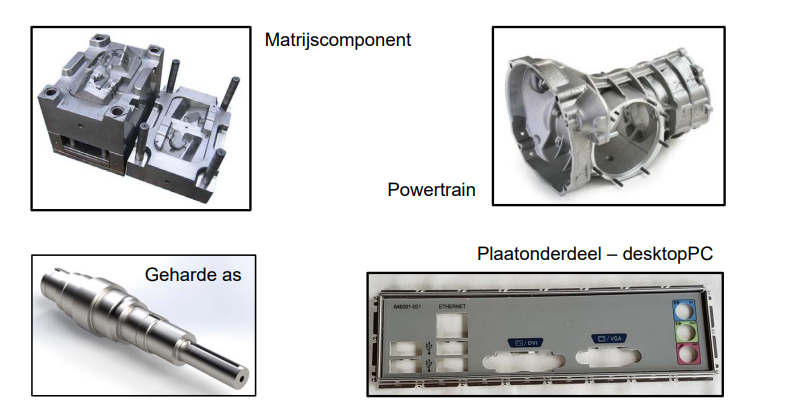
\includegraphics[width=0.65\textwidth]{assets/image84.png}
    \captionof{figure}{Producten die verschillen in complexiteit.}
    \label{fig:lossestukken}
\end{center}

Om een goed plan op te stellen, moet je de eigenschappen (voordelen, nadelen en nauwkeurigheid) kennen van de volgende technieken:
\begin{itemize}
    \item \textbf{Gieten}: Zandgieten, verloren wasmodel, permanent gieten (spuitgieten).
    \item \textbf{Verspanen}: Frezen, draaien en slijpen.
    \item \textbf{Speciale bewerkingen}: Vonkeroderen (EDM), laserbewerking en waterstraalsnijden.
    \item \textbf{Vervormen \& Scheiden}: Ponsen, snijden en kappen.
    \item \textbf{Behandelingen}: Harden en andere warmtebehandelingen.
\end{itemize}

\subsection{Flowchart: Het Werkvoorbereidingsproces}
Onderstaande flowchart geeft een overzicht van de stappen in de werkvoorbereiding, van ontwerp tot productie, met onderscheid tussen de macro- en microfase.

\begin{figure}[htbp]
    \centering
    \begin{tikzpicture}[
            node distance=1.6cm,
            every node/.style={font=\small},
            startstop/.style={rectangle, rounded corners, minimum width=3cm, minimum height=1cm, text centered, draw=black, fill=red!10, thick},
            macro/.style={rectangle, minimum width=3.5cm, minimum height=1cm, text centered, draw=blue!50!black, fill=blue!10, thick},
            micro/.style={rectangle, minimum width=3.5cm, minimum height=1cm, text centered, draw=green!50!black, fill=green!10, thick},
            decision/.style={diamond, aspect=2, minimum width=3cm, minimum height=0.8cm, text centered, draw=black, fill=orange!10, thick},
            arrow/.style={thick,->,>=stealth},
            groupbox/.style={draw=gray, dashed, inner sep=0.5cm, rounded corners, label={[anchor=north west, inner sep=2pt]north west:\textbf{#1}}}
        ]

        % Nodes
        \node (start) [startstop] {Productontwerp (CAD)};
        \node (analysis) [macro, below of=start] {Analyse Geometrie \& Materiaal};

        % Macro Group
        \node (routing) [macro, below of=analysis] {Bepaal Volgorde (Routing)};
        \node (machine) [macro, below of=routing] {Keuze Machines \& Processen};

        % Micro Group
        \node (fix) [micro, below of=machine, yshift=-0.5cm] {Bepaal Opspanning (Fixturing)};
        \node (tools) [micro, below of=fix] {Keuze Gereedschappen};
        \node (params) [micro, below of=tools] {Snijparameters (Snelheid, Voeding)};
        \node (cam) [micro, below of=params] {Genereren Toolpaths (CAM)};

        \node (end) [startstop, below of=cam] {NC Code \& Instructies};

        % Annotations for Macro/Micro
        \node[fit=(routing)(machine), groupbox={Macro Werkvoorbereiding}] (macrogroup) {};
        \node[fit=(fix)(tools)(params)(cam), groupbox={Micro Werkvoorbereiding}] (microgroup) {};

        % Connections
        \draw [arrow] (start) -- (analysis);
        \draw [arrow] (analysis) -- (routing);
        \draw [arrow] (routing) -- (machine);
        \draw [arrow] (machine) -- (fix);
        \draw [arrow] (fix) -- (tools);
        \draw [arrow] (tools) -- (params);
        \draw [arrow] (params) -- (cam);
        \draw [arrow] (cam) -- (end);

    \end{tikzpicture}
    \caption{Flowchart van de werkvoorbereiding: van Macro-beslissingen (procesniveau) naar Micro-beslissingen (operationeel niveau).}\label{fig:werkvoorbereiding_flowchart_detail}
\end{figure}
\FloatBarrier

\begin{warningbox}[EXAMEN CHECKLIST: WERKVOORBEREIDING]
    \begin{itemize}
        \item \textbf{Macro vs. Micro}: Onderscheid beslissingen op procesniveau (routing, machinekeuze) en operationeel niveau (opspanning, tools, parameters).
        \item \textbf{3-2-1 methode}: Leg uit hoe je een werkstuk eenduidig positioneert door vrijheidsgraden te beperken zonder overbepaaldheid.
        \item \textbf{Klemmen}: Begrijp het doel (het tegengaan van proceskrachten) en ken de hulpmiddelen (bankschroef, vacuüm, magneet).
        \item \textbf{CAPP}: Onderscheid de variant methode (GT-gebaseerd) en de generatieve methode (vanaf nul).
        \item \textbf{Referentievlakken}: Begrijp dat alle toleranties afhangen van het gekozen referentievlak en heropspanningen vermeden moeten worden.
    \end{itemize}
\end{warningbox}

\chapter{Productiegericht ontwerpen}
\section{Inleiding}
Productiegericht ontwerpen (Design for Manufacturing, DFM) is het proces waarbij het productontwerp optimaal wordt afgestemd op de beschikbare productieprocessen en fabricagetechnieken. Het doel is om de totale kosten te minimaliseren en tegelijkertijd de kwaliteit en maakbaarheid te verhogen.

Bij een integraal ontwerp kijkt men niet enkel naar de productie, maar ook naar:
\begin{itemize}
    \item \textbf{Design for Assembly (DFA)}: Het ontwerp optimaliseren voor een snelle en foutloze montage.
    \item \textbf{Design for Logistics}: Optimalisatie van verpakking en materiaalstromen.
    \item \textbf{Design for Recycling/Maintenance}: Rekening houden met de volledige levenscyclus, inclusief onderhoud en demontage voor recyclage (Demanufacturing).
\end{itemize}

\begin{figure}[htbp]
    \centering
    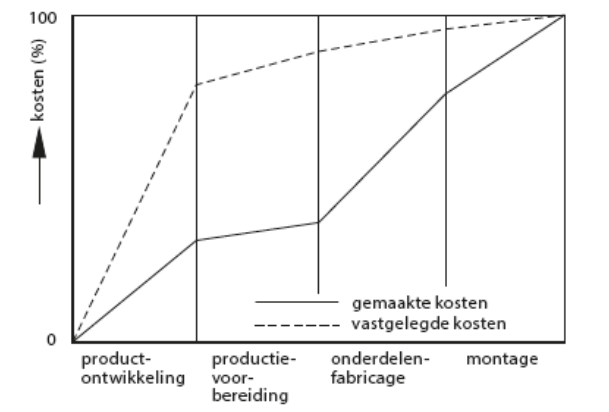
\includegraphics[width=0.45\textwidth]{assets/gemaaktEnVastgelegdeKosten.png}
    \caption{Gerealiseerde versus vastgelegde kosten: Hoewel de ontwerpfase zelf relatief weinig kost, wordt hier het grootste deel van de uiteindelijke productiekosten vastgelegd.}
    \label{fig:gemaaktEnVastgelegdeKosten}
\end{figure}

De ontwerper heeft dus een enorme impact op de uiteindelijke kostprijs door rekening te houden met de functie, maakbaarheid, onderhoudbaarheid en duurzaamheid van het product.

\section{Designen voor verspaanbewerkingen}
In de maakwereld is perfectie onmogelijk.
Een ontwerper moet begrijpen dat gereedschappen hun beperkingen hebben.
Zo is het onmogelijk om een perfecte binnenhoek te frezen met een scherpe rand.
De radius van de frees bepaalt altijd de kleinst mogelijke afronding in de hoek.

\begin{figure}[htbp]
    \centering
    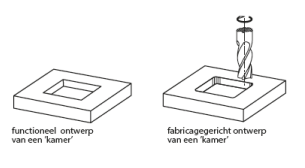
\includegraphics[width=0.4\textwidth]{assets/imperfectiefrezen.png}
    \caption{Beperkingen bij frezen: De radius van het gereedschap maakt het onmogelijk om perfect scherpe binnenhoeken te creëren.}
    \label{fig:imperfectiefrezen}
\end{figure}

\section{Designen voor toeslagen}
Wanneer een product een nabewerking vereist (zoals slijpen na het harden),
moet de ontwerper zorgen dat de betreffende oppervlakken goed toegankelijk zijn voor de bewerkingstools.
Ook moet er voldoende 'toegift' (extra materiaal) voorzien worden, rekening houdend met de toleranties van de voorgaande bewerkingen.

\begin{figure}[htbp]
    \centering
    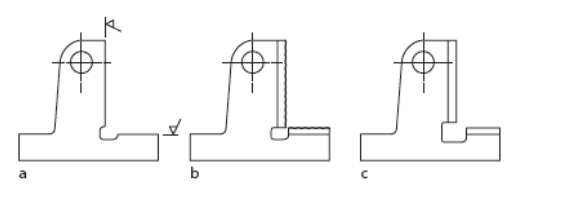
\includegraphics[width=0.6\textwidth]{assets/designenvoortoeslagen.png}
    \caption{Designen voor toeslagen: Het voorzien van voldoende bewerkingstoegift en toegankelijkheid voor gereedschappen.}
    \label{fig:designenvoortoeslagen}
\end{figure}

\section{Designen voor matrijzen}
Bij gieten of spuitgieten moet men rekening houden met de lossing (vrijloophoeken),
een gelijkmatige wanddikte om slink te voorkomen, en het vermijden van ondersnijdingen die de matrijs complex en duur maken.

\section{Algemene regels bij Design for Manufacturing (DFM)}
\begin{itemize}
    \item \textbf{Vermijd scherpe hoeken}: Deze veroorzaken spanningsconcentraties en verhogen het risico op breuk of scheurvorming. Gebruik afrondingen (fillets).

          \begin{figure}[htbp]
              \centering
              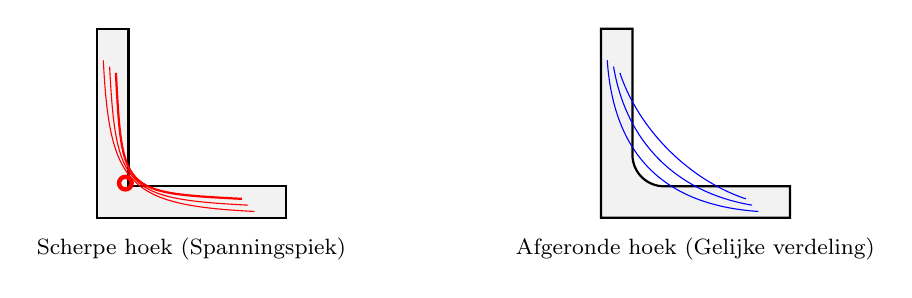
\begin{tikzpicture}[scale=0.8]
                  % Sharp corner
                  \begin{scope}[xshift=-4cm]
                      \draw[thick, fill=gray!10] (0,3) -- (0,0) -- (3,0) -- (3,0.5) -- (0.5,0.5) -- (0.5,3) -- cycle;
                      % Stress lines (concentrated at corner)
                      \draw[red, thin] (0.1, 2.5) .. controls (0.2, 0.5) and (0.5, 0.2) .. (2.5, 0.1);
                      \draw[red, thin] (0.2, 2.4) .. controls (0.3, 0.45) and (0.45, 0.3) .. (2.4, 0.2);
                      \draw[red, thick] (0.3, 2.3) .. controls (0.4, 0.4) and (0.4, 0.4) .. (2.3, 0.3);
                      \draw[red, ultra thick] (0.45, 0.55) circle (0.1); % Point of concentration
                      \node at (1.5, -0.5) {\footnotesize Scherpe hoek (Spanningspiek)};
                  \end{scope}

                  % Rounded corner
                  \begin{scope}[xshift=4cm]
                      \draw[thick, fill=gray!10] (0,3) -- (0,0) -- (3,0) -- (3,0.5) -- (1,0.5) arc(270:180:0.5) -- (0.5,1) -- (0.5,3) -- cycle;
                      % Stress lines (distributed)
                      \draw[blue, thin] (0.1, 2.5) .. controls (0.2, 1) and (1, 0.2) .. (2.5, 0.1);
                      \draw[blue, thin] (0.2, 2.4) .. controls (0.4, 1.2) and (1.2, 0.4) .. (2.4, 0.2);
                      \draw[blue, thin] (0.3, 2.3) .. controls (0.6, 1.4) and (1.4, 0.6) .. (2.3, 0.3);
                      \node at (1.5, -0.5) {\footnotesize Afgeronde hoek (Gelijke verdeling)};
                  \end{scope}
              \end{tikzpicture}
              \caption{Visualisatie van spanningsconcentraties: Een scherpe hoek veroorzaakt een ophoping van spanningslijnen. Een afronding verdeelt de krachten gelijkmatiger.}\label{fig:spanningsconcentratie}
          \end{figure}

    \item \textbf{Minimaliseer het aantal onderdelen}: Hoe minder onderdelen, hoe lager de montagekosten en het risico op fouten.
    \item \textbf{Standaardiseer onderdelen}: Gebruik zoveel mogelijk standaardcomponenten (bouten, lagers) om voorraadkosten te drukken.
    \item \textbf{Modulair ontwerp}: Bouw producten op uit herbruikbare modules die in verschillende configuraties toegepast kunnen worden.
    \item \textbf{Multifunctionele onderdelen}: Probeer meerdere functies te integreren in één onderdeel.
    \item \textbf{Kies realistische toleranties}: Te nauwe toleranties verhogen de kostprijs exponentieel zonder altijd functionele meerwaarde te bieden.
    \item \textbf{Kies goed bewerkbare materialen}: Stem de materiaalkeuze af op de gewenste bewerkingstechniek.
\end{itemize}

\begin{figure}[htbp]
    \centering
    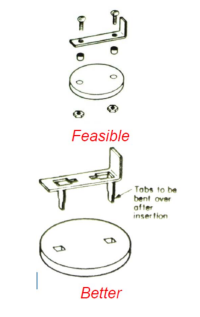
\includegraphics[width=0.3\textwidth]{assets/regelsDFM.png}
    \caption{Overzicht van DFM-regels: Samenvatting van de belangrijkste richtlijnen voor productiegericht ontwerpen.}
    \label{fig:DFMregels.png}
\end{figure}

\begin{conceptbox}[Design for Manufacturing (DFM) vs.\ Manufacturing for Design (MFD)]
    In dit hoofdstuk hebben we telkens beperkingen op het ontwerp gelegd om de productie makkelijker te maken. Dat is DFM.

    MFD is het omgekeerde. Hier ga je kijken naar de productieprocessen en hoe je deze kunt aanpassen om beter aan de ontwerpvereisten te voldoen.
    MFD is duurder, maar duwt de technologie wel vooruit en maakt nieuwe productietechnieken mogelijk.
    3D-printen is bijvoorbeeld ontstaan uit de vraag om eenmalige, specifieke producten makkelijker te maken.
\end{conceptbox}

\begin{warningbox}[EXAMEN CHECKLIST: PRODUCTIEGERICHT ONTWERPEN]
    \begin{itemize}
        \item \textbf{DFM vs. DFA}: Begrijp het verschil tussen ontwerpen voor maakbaarheid en ontwerpen voor assemblage.
        \item \textbf{Scherpe hoeken}: Leg uit waarom afrondingen (fillets) spanningsconcentraties voorkomen.
        \item \textbf{Standaardisatie}: Weet dat standaardonderdelen en modules de kosten en complexiteit verlagen.
        \item \textbf{Impact}: Onthoud dat de ontwerper tot 70-80\% van de uiteindelijke productiekosten vastlegt.
        \item \textbf{Toleranties}: Begrijp dat over-specificeren van toleranties de prijs onnodig opdrijft.
    \end{itemize}
\end{warningbox}

\chapter{Examentips}

Als je een vraag krijgt, wees dan duidelijk in je antwoord.
Schrijf niet enorm grote paragrafen. Een tekening met een korte uitleg is vaak beter.
Bekijk de laatste video op Toledo waarin hij een voorbeeldexamen overloopt.

\chapter{Examenoefeningen}

% TODO: #69 Examenoefeningen toevoegen

\TODO{
    Examenoefeningen toevoegen
}

\chapter{Slotwoord}

Ik heb 4 dagen van de blok gestoken in het maken van deze samenvatting.

Ik hoop dat jullie er veel aan hebben gehad en dat het jullie helpt bij het studeren voor de examens.

\textbf{Ruben out}

\newpage

\chapter*{Succes!}

\vfill

\begin{center}

    \itshape\Huge

    Veel succes met de examens!

    \par\vspace{1cm}

    \normalfont\Large

    --- Ruben Ryckaert

\end{center}



\vspace{3cm}



\begin{quote}

    \centering

    \itshape\Large

    ``Yesterday is history, tomorrow is a mystery, but today is a gift. That is why it is called the present.''

    \par\vspace{0.5cm}

    \textup{--- Oogway}

\end{quote}

\vfill



\end{document}